%/////////////////////////////////////////////////////////////////////
%
% LaTeX definitions:     Ph.D. Dissertation
%                        Nuno Leite
%                        september 2015
%
%/////////////////////////////////////////////////////////////////////


\documentclass[12pt, a4paper, openright, twoside]{report}



%////////////
% Acronyms
% Load the package with the acronym option. Omit the dot at the end of each description
\usepackage[acronym,nomain,toc,nopostdot]{glossaries}
% Suppress acronym bold font
\renewcommand*{\glsnamefont}[1]{\textmd{#1}}

% For resetting acronyms at the beginning of each chapter
\usepackage{etoolbox}
\preto\chapter\glsresetall

%
\usepackage{glossaries-extra}
\renewcommand{\glsfirstlongdefaultfont}[1]{\emph{#1}}
\setabbreviationstyle[acronym]{long-short}
%

% Redefining indentation in the List of acronyms
\newglossarystyle{super3colleft}{%
  \renewenvironment{theglossary}%
    {\tablehead{}\tabletail{}%
     \begin{supertabular}{@{}>{\bfseries}lp{\glsdescwidth}p{\glspagelistwidth}}}%
    {\end{supertabular}}%
  \renewcommand*{\glossaryheader}{}%
  \renewcommand*{\glsgroupheading}[1]{}%
  \renewcommand*{\glossaryentryfield}[5]{%
    \glsentryitem{##1}\glstarget{##1}{##2} & ##3 & ##5\\}%
  \renewcommand*{\glossarysubentryfield}[6]{%
     &
     \glssubentryitem{##2}%
     \glstarget{##2}{\strut}##4 & ##6\\}%
  \renewcommand*{\glsgroupskip}{ & &\\}%
}



\newlength{\acronymlabelwidth}
\setlength{\acronymlabelwidth}{0.25\textwidth}
%////////////

% Chapter style
\usepackage[Lenny]{fncychap}

% Chapter minitoc
\usepackage{minitoc}

% English language
\usepackage[english]{babel}
\usepackage[T1]{fontenc}
%\usepackage[latin1]{inputenc}
\usepackage[utf8]{inputenc}

% Times New Roman typeface
%\usepackage{textcomp}
\renewcommand{\rmdefault}{ptm} % set Times as the default text font
% If AMS-LaTeX is used, it can be loaded before or after mtpro2
\usepackage{amsmath}		
%% The following loads mtpro and defines some common MTPro options 
%\usepackage[subscriptcorrection, slantedGreek, nofontinfo]{mtpro2}

% My styles
\usepackage{myStyles}


% Graphics package
%\usepackage[dvips]{graphicx}
\usepackage{graphicx}

% Other packages
\usepackage{epsfig}
\usepackage[nottoc]{tocbibind} % To include bibliography in TOC
\usepackage{latexsym}
% Fancy headers
\usepackage{fancyhdr}




%////////////// ADDED PACKAGES //////////////////
%\usepackage{natbib,hyperref} % For numerical format
\usepackage[natbibapa]{apacite} % For APA format
\usepackage{hyperref}
\usepackage{graphics} % resizebox command
\usepackage[toc,page]{appendix} % For defining appendices
\PassOptionsToPackage{hyphens}{url} % For processing correctly underscores in URL
\usepackage{subfigure}
\usepackage{calc}
%\usepackage{amssymb} % MTPro2 fonts contain all of the symbols provided by amssymb. 
% The amsthm package provides extended theorem environments
% \usepackage{amsthm}
\usepackage{amstext}
\usepackage{amsmath}
\usepackage{textcomp} % degree symbol 
\usepackage{graphicx}
%///
% Algorithm package
\usepackage[chapter]{algorithm}
%\usepackage{algorithmicx}
\usepackage{algpseudocode} % Typesetting using the algorithmicx package
% Algorithm numbering
\renewcommand{\thealgorithm}{\arabic{chapter}.\arabic{algorithm}} 
%///

\usepackage{lineno} % linenomath

% Allow break in align math environment
\allowdisplaybreaks

\usepackage{eqparbox,array}

\newcommand\LONGCOMMENT[1]{%
	\hfill$\triangleright$ \begin{minipage}[t]{15\eqboxwidth{algorithmiccomment}}#1\strut\end{minipage}%
}

\newcommand\LONGCOMMENTONE[1]{%
	\hfill$\triangleright$ \begin{minipage}[t]{14\eqboxwidth{algorithmiccomment}}#1\strut\end{minipage}%
}

\newcommand\LONGCOMMENTTWO[1]{%
	\hfill$\triangleright$ \begin{minipage}[t]{17\eqboxwidth{algorithmiccomment}}#1\strut\end{minipage}%
}

% For floating point columns
\usepackage{etoolbox} 
\usepackage[tight-spacing=true]{siunitx}
\robustify\bfseries
% For bold cells using siunitx
\newcommand{\be}[2]{%
	\multicolumn{1}{S[table-format=#1,
		mode=text,
		text-rm=\fontseries{b}\selectfont
		]}{#2}}

% For bold cells using siunitx
\newcommand{\beIt}[2]{%
	\multicolumn{1}{S[table-format=#1,
		mode=text,
		text-rm=\fontseries{b}\fontshape{it}\selectfont
		]}{#2}}

% For bold cells using siunitx
\newcommand{\beSci}[1]{%
	\multicolumn{1}{
		S[table-format =1.2e4,%    
%		S[exponent-product = \cdot,
%		round-mode = figures,
%		round-precision = 3,
		detect-weight=true, 
		detect-family=true,
		mode=text,
		text-rm=\fontseries{b}\selectfont
		]}{#1}}

%\usepackage[tight-spacing=true]{siunitx}

\usepackage{booktabs} % Professional tables
% Use in coloured tables
\usepackage{cancel}
\usepackage[pdftex, table]{xcolor}  % Coloured text etc.
%To tweak the space between columns (LaTeX will by default choose very tight columns), one can alter the column separation: \setlength{\tabcolsep}{5pt}. The default value is 6pt.
\setlength{\tabcolsep}{5pt}
%\setlength{\tabcolsep}{1.7pt}
\usepackage{todonotes}
\usepackage{multirow}
\usepackage{pdflscape}
\usepackage{enumerate}
\usepackage{stfloats} % TA plots
\usepackage{adjustbox}
\usepackage{longtable} % For long tables spanning multiple pages

% For removing underfull \hbox warning in the bibliography
\apptocmd{\sloppy}{\hbadness 10000\relax}{}{}
% Alternatively
%\usepackage{etoolbox}
%\apptocmd{\thebibliography}{\raggedright}{}{}

\usepackage{float}
\floatstyle{plaintop}
\restylefloat{table}

%\newcommandx{\info}[2][1=]{\todo[linecolor=OliveGreen,backgroundcolor=OliveGreen!25,bordercolor=OliveGreen,#1]{#2}}

\newif\ifboldnumber
\newcommand{\boldnext}{\global\boldnumbertrue}

% Default definition is \footnotesize#1:
\algrenewcommand\alglinenumber[1]{%
	\footnotesize\ifboldnumber\bfseries\fi\global\boldnumberfalse#1:}

\usepackage{verbatimbox}

\newcolumntype{L}[1]{>{\raggedright\let\newline\\\arraybackslash\hspace{0pt}}m{#1}}


\usepackage{doi}
\renewcommand\doitext{} % Remove duplicate "doi:" prefix
% For placing figures and tables in the next page
\usepackage{afterpage}
\usepackage{flafter}
% siunitx EN language floating point separator
\sisetup{group-separator = {,}}

% For reducing \hbox warnings
\sloppy

%////////////////////////////////////////////////


\usepackage{setspace}
\onehalfspacing % or \doublespacing

% Line spacing
%\linespread{1.25} %// LAST
%\linespread{1.35}
%\linespread{1.4}

% Page dimensions - equivalent to 15 cm x 23 cm
\usepackage[left=3.5cm,right=2.5cm,top=3cm,bottom=3.7cm]{geometry}

%\usepackage[headheight=14pt, text={15cm,23cm}, twoside, bindingoffset=1cm]{geometry}

%\usepackage[headheight=14pt, text={15cm,23cm}, top=2cm, left=2.5cm, right=2.5cm, bottom=2.5cm, twoside, bindingoffset=1cm, includefoot, includehead]{geometry}

% Page dimensions
%\pagestyle{plain}
%\setlength{\oddsidemargin}{0.5cm} 
%\setlength{\evensidemargin}{-0.5cm}
%\setlength{\topmargin}{-1cm} 
%\setlength{\textheight}{23cm}
%\setlength{\textwidth}{16cm}
%



%-
% //////// Changing default figure captions ///////
%-
%\setlength{\abovecaptionskip}{10pt}
\setlength{\belowcaptionskip}{5px}


%\makeatletter % Allow the use of @ in command names
%\long\def\@makecaption#1#2{%
%\vskip\abovecaptionskip
%\sbox\@tempboxa{ \textbf{#1} \hspace{0.5em} #2}%
%\ifdim \wd\@tempboxa >\hsize
%{ \textbf{#1} \hspace{0.5em}  #2\par}
%\else
%\hbox to\hsize{\hfil\box\@tempboxa\hfil}%
%\fi
%\vskip\belowcaptionskip}
%\makeatother % Cancel the effect of \makeatletter 
%% ////////////////////////////
%
%% //// Use 'Computer Modern' typewriter font, not 'Lucida Typewriter' ////
%\renewcommand{\ttdefault}{cmtt}%
%% //// Estilo adoptado para trocos de codigo no texto ////
%\newcommand{\code}[1]{{\tt #1}}



% ///// Fancy headers ////////
\usepackage{fancyhdr}
\pagestyle{fancy}
\fancyhf{}

\renewcommand{\chaptermark}[1]{%
  \markboth{\chaptername \ \thechapter \hspace{0.5em} \emph{#1}}{}}

\renewcommand{\sectionmark}[1]{%
  \markright{\thesection \hspace{0.5em} #1}{}}
     
\renewcommand{\headrulewidth}{0pt}

\fancypagestyle{plain}{%
\fancyhf{} % clear all header and footer fields
\fancyfoot[C]{\small\thepage} % except the center
\renewcommand{\headrulewidth}{0pt}
\renewcommand{\footrulewidth}{0pt}}
% /////////////////////////////////


% Load acronym definitions
\loadglsentries[\acronymtype]{Acronyms/Acronyms}

% Generate the glossary
\makeglossaries


\usepackage{silence}

\WarningFilter{minitoc(hints)}{W0023}
\WarningFilter{minitoc(hints)}{W0028}
\WarningFilter{minitoc(hints)}{W0030}

\WarningFilter{blindtext}{} % this takes care of the `blindtext` messages




%//////////////////////////
%
% Main matter
%
%//////////////////////////
\begin{document}

% Environment for displaying examples
%\theoremstyle{definition}
\newtheorem{exmp}{Example}[section]


% Commands
\renewcommand\bibname{References}


% Document cover
\thispagestyle{empty}

\begin{figure}[ht!]
	%\vspace*{-4cm}
	\centering
	\scalebox{0.6}{
\includegraphics{FrontCover/Logo_ISEL}}
\end{figure}


\centerline{\Large\textbf{INSTITUTO POLIT\'{E}CNICO DE LISBOA}}
\bigskip
%\bigskip
\centerline{\Large\textbf{INSTITUTO SUPERIOR DE ENGENHARIA DE LISBOA}}


\bigskip
\bigskip

\title{{\large Licenciatura em Engenharia de Inform\'{a}tica e de Computadores}}

\bigskip
\bigskip

\begin{center}

 
{\LARGE \textbf{PostChat}}

\bigskip
{\Large \textbf{"Bring Back Postcards"}}

\bigskip
\bigskip
\bigskip
\bigskip
\bigskip
\bigskip
\bigskip
\bigskip



{\Large \textbf{\vspace*{1em}Ant\'{o}nio Carvalho n.\textdegree $\ $48347}}

{\Large \textbf{e-mail: \texttt{a48347@alunos.isel.pt}}}

\bigskip
\bigskip
\bigskip
\bigskip

{\Large \textbf{\vspace*{1em}Supervisor:} Nuno Leite} 



\bigskip
\bigskip
\bigskip




{\Large Report}

\bigskip
\bigskip


{\Large Projeto e Semin\'{a}rio - June 2023}


\end{center}
 

\clearpage
\thispagestyle{empty}
\cleardoublepage



% Begin with roman numbering at page 3 (provisory document)
\pagenumbering{roman} \setcounter{page}{3}
%\pagenumbering{roman} \setcounter{page}{5}



% Fancy Header configuration

% Formato da pagina esquerda (par): <Pagina><Capitulo nr Nome>
\fancyhead[LE]{\small\thepage\hspace{3em}\nouppercase{\small\leftmark}}
\fancyhead[RE,LO]{}
% Formato da pagina direita (impar): <Numero da Seccao> <Nome da seccao> <Pagina>
\fancyhead[RO]{\nouppercase{\small\rightmark}\hspace{3em}\small\thepage}

\setlength{\headheight}{13.60pt}


% //////// ORIENTACAO DA TESE //////////////
%\typeout{}
%\include{../Orientation/Orientation}
%
%\newpage \mbox{}    % Blank page.
% //////////////////////////////////////////


% English Abstract
\typeout{Abstract}

\prefacesection{Abstract}



\vspace{3em}

\noindent

There is a large library of platforms and apps that allow one to invite people to an event. These platforms, however, have some downsides, for example, splitting expenses of an event is hard to do on those platforms, they require new users to make an account and activating it, are not available on multiple platforms, among other issues. The goal of this project is to develop a new platform that tackles these disadvantages. This way the group implemented a new solution using modern platforms (such as ASP.NET CORE and Xamarin) that can be used by a large number of people on modern devices and can later be expanded to new environments that might be created. The group was presented with some challenges that had to be overcome, like the authentication without account creation using multiple providers, the notifications mechanism, or the code sharing between platforms. The result is a new application supported by a Web API without the need to create a new account on another platform, using the already existing accounts on other services like Facebook and Microsoft’s Outlook, for example.


\vspace*{1em}

\textbf{\large{Keywords:}} Events, Item, Task, User, Invitation.


%\begin{itemize}
%	
%	
%	\item Events - Something that takes place (in this case social events);
%	\item Item - Associated with events, these are the objects of an event;
%	\item Task - An action that needs to be done by a participant in an Event;
%	\item User - Person that uses the platform, normally comprised of a Name, Email and Phone Number;
%	\item Invite - Asking for someone to go to an Event.
%	
%\end{itemize}

%
%
%\cleardoublepage
%
%
%\prefacesection{Acronyms}
%
%
%
%\vspace{3em}
%
%\noindent
%
%%\textbf{\large{Acronyms:}} 
%
%\acrshort{orm} stands for \acrfull{orm}.
%
%\acrshort{crud} stands for \acrfull{crud}.
%
%\acrshort{ide} stands for \acrfull{ide}.






%\newpage \mbox{}    % Blank page.


% Portuguese Abstract
%\typeout{Resumo}
%



\prefacesection{Resumo}





\vspace{3em}
%\vfill{}

\noindent
\textbf{\large{Palavras-chave:}} Keyword 1, Keyword 1, ... .

%\newpage \mbox{}    % Blank page.


% Acknowlegdments
%\typeout{Acknowledgements}
%

\prefacesection{Acknowledgements}


I would like to thank to the people and the institutions directly involved in this work.

To ....
Finally, I would like to thank my family. ....




%\newpage \mbox{}    % Blank page.
%
%
%% //////// Dedication //////////////
%\typeout{}
%


\vspace*{8em}


\hspace*{\fill} {\large \textit{To ...}}

\vspace*{4em}

\hspace*{\fill} {\large \textit{To ...}}

%\newpage \mbox{}    % Blank page.
% //////////////////////////////////////////


%% //////// List of Acronyms and Abbreviations //////////////
%%\printglossary[type=\acronymtype,nonumberlist=true]
%{\typeout{List of Acronyms and Abbreviations} 
%


%%/////////////////////////////////////////////////
% Acronym definitions
% <key> <acronym> <description>
\newacronym{crud}{CRUD}{Create, Read, Update and Delete}
\newacronym{test}{TEST}{Test, Extreme, Stupid, Test}
\newacronym{svg}{SVG}{Scalable Vector Graphics}
\newacronym{sms}{SMS}{Short Messaging Service}
\newacronym{tts}{TTS}{Text To Speech}
\newacronym{htr}{HTR}{Handwriten Text Recognition}
\newacronym{uri}{URI}{Uniform Resource Identifier}
\newacronym{rdbms}{RDBMS}{Relational Database Management System}
\newacronym{png}{PNG}{Portable Network Graphics}
\newacronym{jvm}{JVM}{Java Virtual Machine}
\newacronym{ai}{AI}{Artificial Inteligence}
\newacronym{rest}{REST}{REpresentational State Transfer}
\newacronym{http}{HTTP}{Hypertext Transfer Protocol}
\newacronym{api}{API}{Application Programming Interface}
%%/////////////////////////////////////////////////







}
%
%\newpage \mbox{}    % Blank page.
%% //////////////////////////////////////////

% List of Acronyms with no page numbers
%\printglossary[title=List of Acronyms,toctitle=List of Acronyms,nonumberlist=true]

% List of Acronyms with no page numbers and custom indentation between acronym and description
\printglossary[title=List of Acronyms,toctitle=List of Acronyms,nonumberlist=true,type=\acronymtype,style=super3colleft]


\cleardoublepage


%
%% //////// Notational Conventions //////////////
%{\typeout{Notational Conventions}
%%\vspace{1cm}
%\begin{flushleft} 
%\fontsize{16}{24}\textbf{Lista de Acrónimos} 
%\end{flushleft} 
%\vspace{1cm}
\prefacesection{List of Symbols and Notation}
\vspace{-2cm}
The most frequent symbols and notation are as follows.
\hrule
\begin{table}[h]
\begin{tabular}{@{}l@{\hspace{.5cm}}l} \\
$c,$	 		& number of different classes in a dataset \vspace{-2mm} \\
$d,$	 		& dimensionality or number of features in a dataset \vspace{-2mm} \\
$L,$ 			& cumulative threshold for feature selection \vspace{-2mm} \\
$m,$	 		& number of selected features \vspace{-2mm} \\
$M_S,$    & maximum allowed similarity \vspace{-2mm} \\  
$n,$	    & number of instances in a dataset \vspace{-2mm} \\
$q,$      & maximum number of bits to discretize a given feature \vspace{-2mm} \\
$s,$      & number of sampled instances from a dataset \vspace{-2mm} \\ 
${\bf x}_i,$  & the $i$-th feature vector $\in \mathbf{R}^d$ \vspace{-2mm} \\ 
$X_i,$ & feature $i$ with $i \in \{1,\ldots,d\}$ \vspace{1cm} \\ 

$\eta,$   & percentage of features to keep in the DDF and the DDW methods \vspace{-2mm} \\
$\ell_0,$ & $\ell_0$ norm for a vector \vspace{-2mm} \\
$\Delta,$  & maximum allowed distortion \vspace{1cm} \\

$\mathcal{D},$ & dataset \vspace{-2mm} \\
$\mathcal{X, Y},$   & random variable \vspace{1cm} \\

$H(.),$ & entropy of a random variable \vspace{-2mm} \\
$H(.|.),$ & conditional entropy of one random variable given another \vspace{-2mm} \\
$I(.),$  & self-information of a specific random variable outcome \vspace{-2mm} \\
$I(.;.),$  & mutual-information between a pair of random variables \vspace{-2mm} \\

\end{tabular}
\end{table}



} % Blank page.
%% //////////////////////////////////////////
%
%
%% //////// List of Symbolss //////////////
%{\typeout{List of Symbols}
%\include{Other/ListOfSymbols}} % Blank page.
%% //////////////////////////////////////////
%



%///////////////////////////////////////////////
%
% Contents
% List of Figures
% List of Tables
% List of Algorithms
%
%///////////////////////////////////////////////
\dominitoc
\tableofcontents 
\listoffigures 
%\listoftables   
%\listofalgorithms \addcontentsline{toc}{chapter}{List of Algorithms} 

\cleardoublepage

% Arabic numbering
\pagenumbering{arabic}




%////////////////////////////////////////////////////////////////////////
%   Chapter 1
%
%   Introduction
%////////////////////////////////////////////////////////////////////////
% Se contiver Resumo e Abstract
\setcounter{mtc}{3} % First page containing the minitoc

% Se contiver Abstract apenas
%\setcounter{mtc}{6} % First page containing the minitoc




\chapter{Introduction} 
\label{ch:Chapter1}
\vfill \minitoc \newpage


While there are some applications that allow for the creation of events, invitations and publishing, none of them focus on what really happens during and in the planning of an event.

In a real case scenario like the organization of a \textit{party} type of event, there are some important factors to take into account. For this type of events it's possible to list some basic needs like: budget management (expenses like food and drinks), location, or entertainment (such as music).

The purpose of this project consists of simplifying the planning and management of events having the focus on people collaboration through a mobile application, while keeping it possible to expand to other platforms.

The proposed solution is comprised of a Web API and a client application. The Web API is supported by .NET CORE MVC and a PostgreSQL SQL database engine. The client application is built using Xamarin Forms, with aim especially for Android devices and Windows devices. All operations (such as creating events, items, tasks, etc...) happen in the API and the client application communicates with it using HTTP.

The remainder of the report is organized in seven chapters. Chapter 2 presents the State of the Art. In Chapter 3, the project functionality is presented. Chapter 4 describes the development support used in the project. In Chapter 5 the project roadmap is analyzed. Chapter 6 draws some conclusions and gives pointers to future work.






%////////////////////////////////////////////////////////////////////////
%   Chapter 2 
%
%   State of the Art
%////////////////////////////////////////////////////////////////////////

\chapter{State of the art} 
\label{ch:Chapter2}
\vfill \newpage

In today's digital landscape, several messaging apps compete to provide users with a platform for connecting and sharing personalized messages. This chapter aims to compare PostChat with messaging and postcard apps such as \textit{\cite{WhatsApp}}, \textit{\cite{Telegram}}, and \textit{\cite{MyPostcard}}, highlighting PostChat's state-of-the-art qualities and distinct features over these apps. By analyzing their design, usability, and user experience, we can gain insights into PostChat's unique position, distinct idea, and what it borrows from its contemporaries.


\textit{PostChat}, much like WhatsApp or Telegram, prioritizes a user-friendly design and intuitive navigation. Its interface is simple and streamlined, ensuring a seamless postcard creation and sending experience for users of all ages. Also like those apps, it allows to create groups but instead of sending messages it sends postcards.

Unlike WhatsApp or Telegram, PostChat is focused on sending postcards and has a set of simple and straight forward drawing tools, high quality postcard templates and AI assisting tools that distinguish it from those other apps. 

MyPostcard has a different approach as it allows users to fully customize a postcard via a digital interface but send the postcard via physical mail, that is, no chat groups, no way to find friends in the service, just plain address form filling. PostChat approach allows for both formats as it send the digital postcards and can export them in order to printed onto physical paper.

In conclusion \textit{PostChat} borrows elements from different apps and makes a unique 
format for itself opening doors for a new way of communication and a new possible business 
opportunity.


%////////////////////////////////////////////////////////////////////////
%   Chapter 3
%
%   
%////////////////////////////////////////////////////////////////////////
\chapter{Requirements}
\label{ch:Chapter3}
\vfill \minitoc \newpage

\section{Functional Requirements}
In this section we will delve in to the requirements needed to implement this project. %complete


\subsection{Mandatory Requirements}

The mandatory functional requirements are the following:
\begin{itemize}
    \item Editing and personalizing a postcard

	\item Sending and receiving postcards;
	
	\item Creating chat groups;
	
	\item Connecting to all friends in the service via user's stored phone number;
	
	\item Export a postcard in high quality;

    \item Build and train a Handwriting Text Recognition model.
\end{itemize}


\subsection{Optional Requirements}

\begin{itemize}
        \item Use a \gls{tts} implementation to read the postcard out loud;
        \item Using \gls{sms} based verification;
\end{itemize}

\bigskip 

\section{Overview}
\noindent

PostChat has simple and intuitive functionalities. In this chapter is shown a overview of the service, detailed explanation of every component will be provided later in this report.

\subsection{Project Architecture}
PostChat has a client made for Android using Jetpack Compose framework a server programmed in Kotlin using the Spring framework and running in the \gls{jvm}. The same server creates processes to call the \gls{ai} \gls{htr} model made in Python and uses a PostgreSQL database to store data. 

\begin{figure}[!ht]
	\centering
	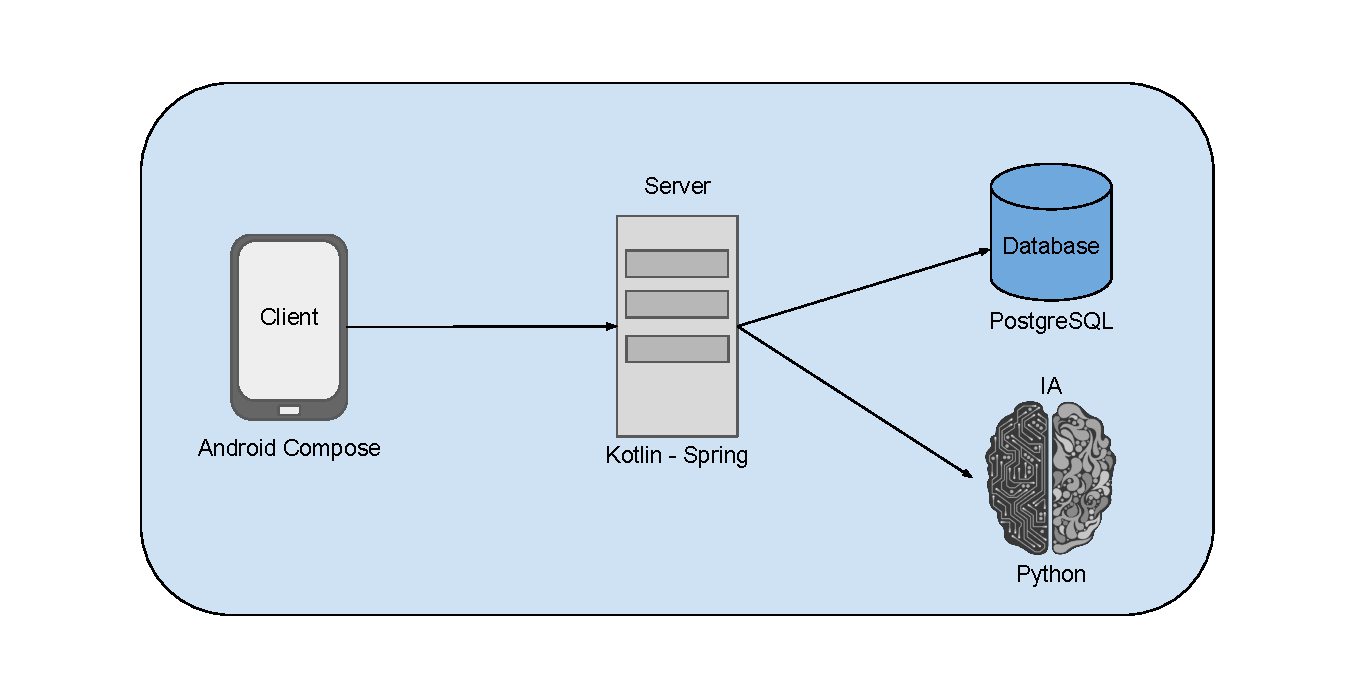
\includegraphics[width=0.9\textwidth]{./Chapter3/Figures/Project Structure}
	\caption{Project Architecture}
	\label{fig:PStruct}
\end{figure}


\subsection{Signing In}
To be able to use any of the provided functionalities its necessary for the user to sign in the service. Signing In can be either a login operation or a register operation. Its required for the user to have a valid phone number in order to perform either one of the operations.
Once registered the user will have access to all of the service functionalities.

\subsection{Connecting to Friends}
Connecting to friends in the service is simple, no need to find for a specific username simply give access to the user's phone numbers and the service will provide you with the contacts registered in it.   

\subsection{Obtaining Templates}
A template represents a potential postcard background. Every application developed to use this Web API needs to have consistency, that is, it needs to keep the templates up-to-date with the ones stored in the server.


\subsection{Creating Chat Groups}
Once registered the user can now create chats groups. These chat groups are made up of all the people the users is meant to send a postcard and/or receive from.
When sending a postcard to someone a chat group is required.  

\subsection{Sending Messages (Postcards)}
A message is referenced in this report and throughout the application development as a holder for the postcard. A message contains more information besides the postcard itself (we will delve deeper about messages in the report \ref{subsec:Message}).
Sending a postcard involves choosing a postcard template (the background of the postcard) and  writing to it. 
Internally the postcard is represented by two layers, the template and the written content, both of which are SVG's \textit{\cite{SVG}}, allowing for high quality postcards. 

\subsection{Handwriting Text Recognition}
For each message a request can be made to extract the drawn text contained in it to computer digits. To perform such operation only the drawn content is needed.

\bigskip

\paragraph{Application Flow}

The application flow can be seen in Figure~\ref{fig:AppFlow}.

\begin{figure}[!ht]
	\centering
	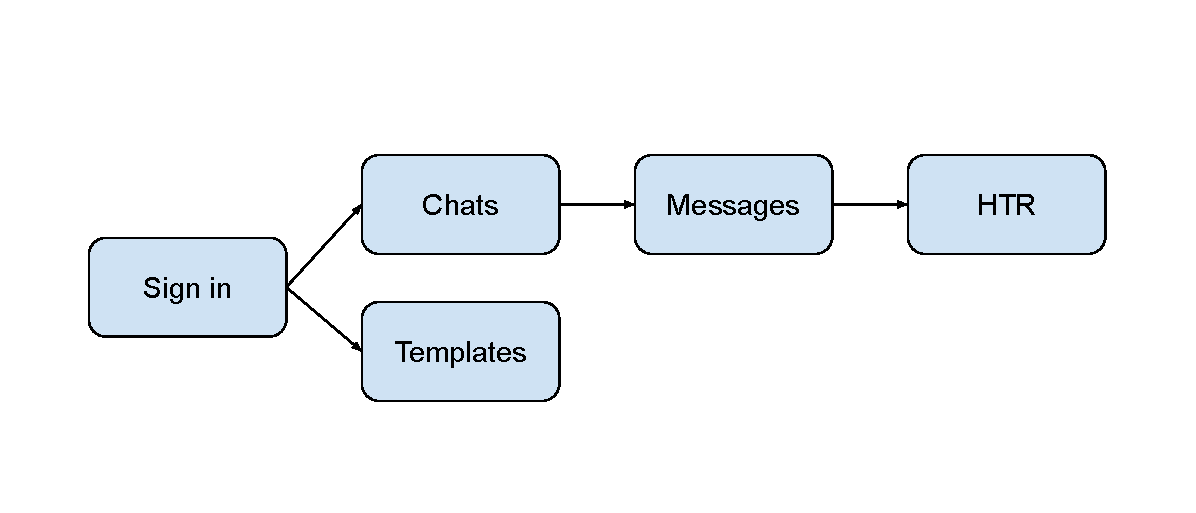
\includegraphics[width=0.75\textwidth]{./Chapter3/Figures/Application Flow}
	\caption{Application Flow}
	\label{fig:AppFlow}
\end{figure}


%////////////////////////////////////////////////////////////////////////
%   Chapter 4
%
%   
%
%////////////////////////////////////////////////////////////////////////
\chapter{Development support} 
\label{ch:Chapter4}
\vfill \minitoc \newpage

\section{Azure DevOps Services}

To ease development the group decided to use \textit{\cite{azuredevops}}. This platform provides development collaboration tools along with mechanisms that allow for a better work environment that follow DevOps practices.

Figure~\ref{fig:DevopsTasks1} illustrates DevOps Work Items (Azure Boards).

From the many tools provided by the service, the following are the ones used in this project:
\begin{itemize}
	\item Azure Boards
	\item Azure Repos
	\item Azure Pipelines
	\item Azure Artifacts
\end{itemize}


\begin{figure}[!ht]
	\centering
	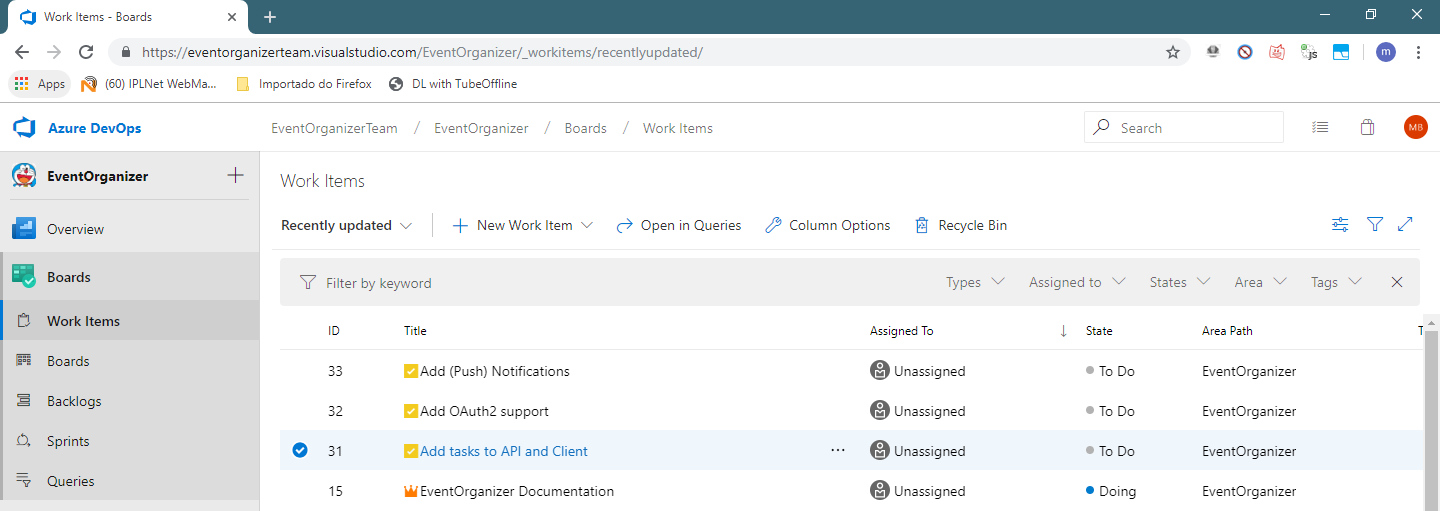
\includegraphics[width=0.75\textwidth]{./Chapter4/Figures/DevopsTasks1.png}
	\caption{DevOps Boards Work Items}
	\label{fig:DevopsTasks1}
\end{figure}

\subsection{Azure Repos}
Azure Repos is a set of version control tools, allowing for multiple repositories, each one having its own version control system. For this project four repositories where created:

\begin{itemize}
	\item EventOrganizer.WebApi – Where the source code for the EventAPI and its HTTP Client is maintained.
	\item EventOrganizer.Client – Where the Xamarin client application source code is maintained.
	\item EventOrganizer.Database – Repository containing the scripts and backups for database management.
	\item EventOrganizer.Documentation – Dedicated to gather project documentation used in development.
	\item EventOrganizer.MusicApi – Contains the source code for the Music Web Api and its HTTP Client.
\end{itemize}

Figure~\ref{fig:BranchingStrategy} illustrates the feature branching strategy used.

Wanting to keep the development repositories, EventOrganizer.WebApi, EventOrganizer.MusicApi and EventOrganizer.Client organized and easy to maintain, the group decided to use the following branching strategy:

\begin{figure}[!ht]
	\centering
	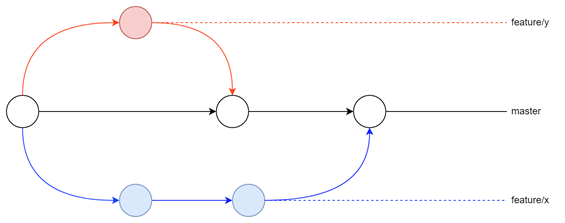
\includegraphics[width=0.75\textwidth]{./Chapter4/Figures/BranchingStrategy.png}
	\caption{Feature Branching Strategy}
	\label{fig:BranchingStrategy}
\end{figure}

This branching strategy consists of creating a feature branch for each new functionality that needs to be implemented. This, combined with frequent pull requests, helped the team maintaining the source code, making sure the master branch always had a stable version and making bugs less frequent and smaller problems to resolve.

\subsection{Azure Pipelines}
Azure Pipelines is a service that can be used to build, test and deploy projects by having remote machines run a preconfigured pipeline.

For this project the group configured three pipelines:

\begin{itemize}
	\item Event Web API Pipeline – Builds the EventAPI project and deploys the Web API to Azure App Services.
	\item Generate Client Nugets – Builds and packages the EventAPI HTTP client libraries into nuget packages that contain versioning.
	\item Event Web API Pipeline – Builds the EventAPI project and deploys the Web API to Azure App Services.
	
\end{itemize}

The first two pipelines are queued for execution every time there is a new stable version, meaning every time there is a push to the master branch.

\subsection{Azure Artifacts}
Azure Artifacts gave the team the possibility of having a private nuget feed where the nuget packages generated in the Azure Pipelines are automatically pushed. This service comes with a page in Azure DevOps, where the nugets can also be viewed and managed.

\subsection{Pull Requests}

To keep code versioning efficient and organized, the decision to block direct pushes to the master branch was made.

When a feature is complete, instead of merging the feature branch to the master branch, a pull request must be open and reviewed before being completed, which results in an automatic merge to the master branch.

In addition to the mandatory review of the code, pull requests must also pass a build pipeline configured for each repository. This was done by first creating a new Azure Pipeline for each repository that builds and tests the respective solutions and secondly adding a build policy for the master branch, which specifies that the previously created pipeline should run to completion successfully.

The page for a pull request where the required policies include the previously mentioned code review, build and test run can be seen in the screen capture below.

\begin{figure}[!ht]
	\centering
	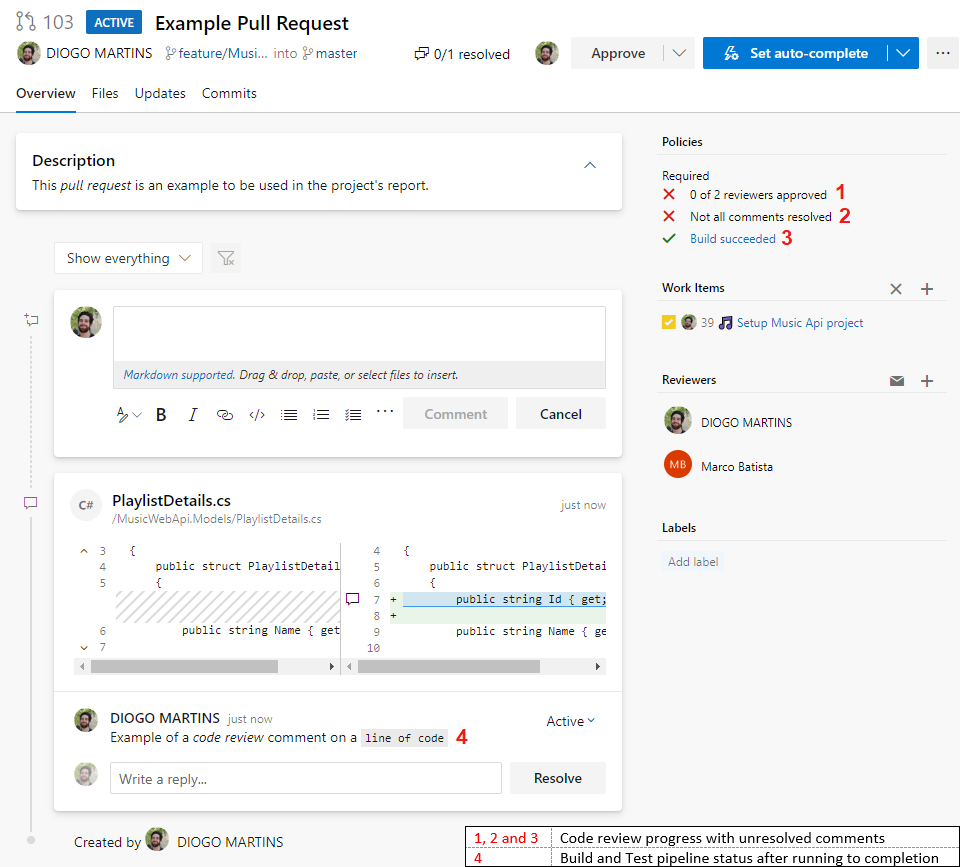
\includegraphics[width=0.75\textwidth]{./Chapter4/Figures/PullRequestExample.png}
	\caption{An example of a pull request in the development repositories}
	\label{fig:PullRequestExample}
\end{figure}

\newpage

\section{Other tools}
The group is also using Microsoft Visual Studio as it's main programming IDE as it's really flexible and it's integration with Nuget, Xamarin and UWP is seamless to the group and offers (almost) no problems and Jetbrains DataGrip as the main database IDE (although sometimes the group also uses pgAdmin for more low level operations on the PostgreSQL database).



\section{Architecture}

Figure~\ref{fig:SystemArchitecture} illustrates the system architecture.

\begin{figure}[!ht]
	\centering
	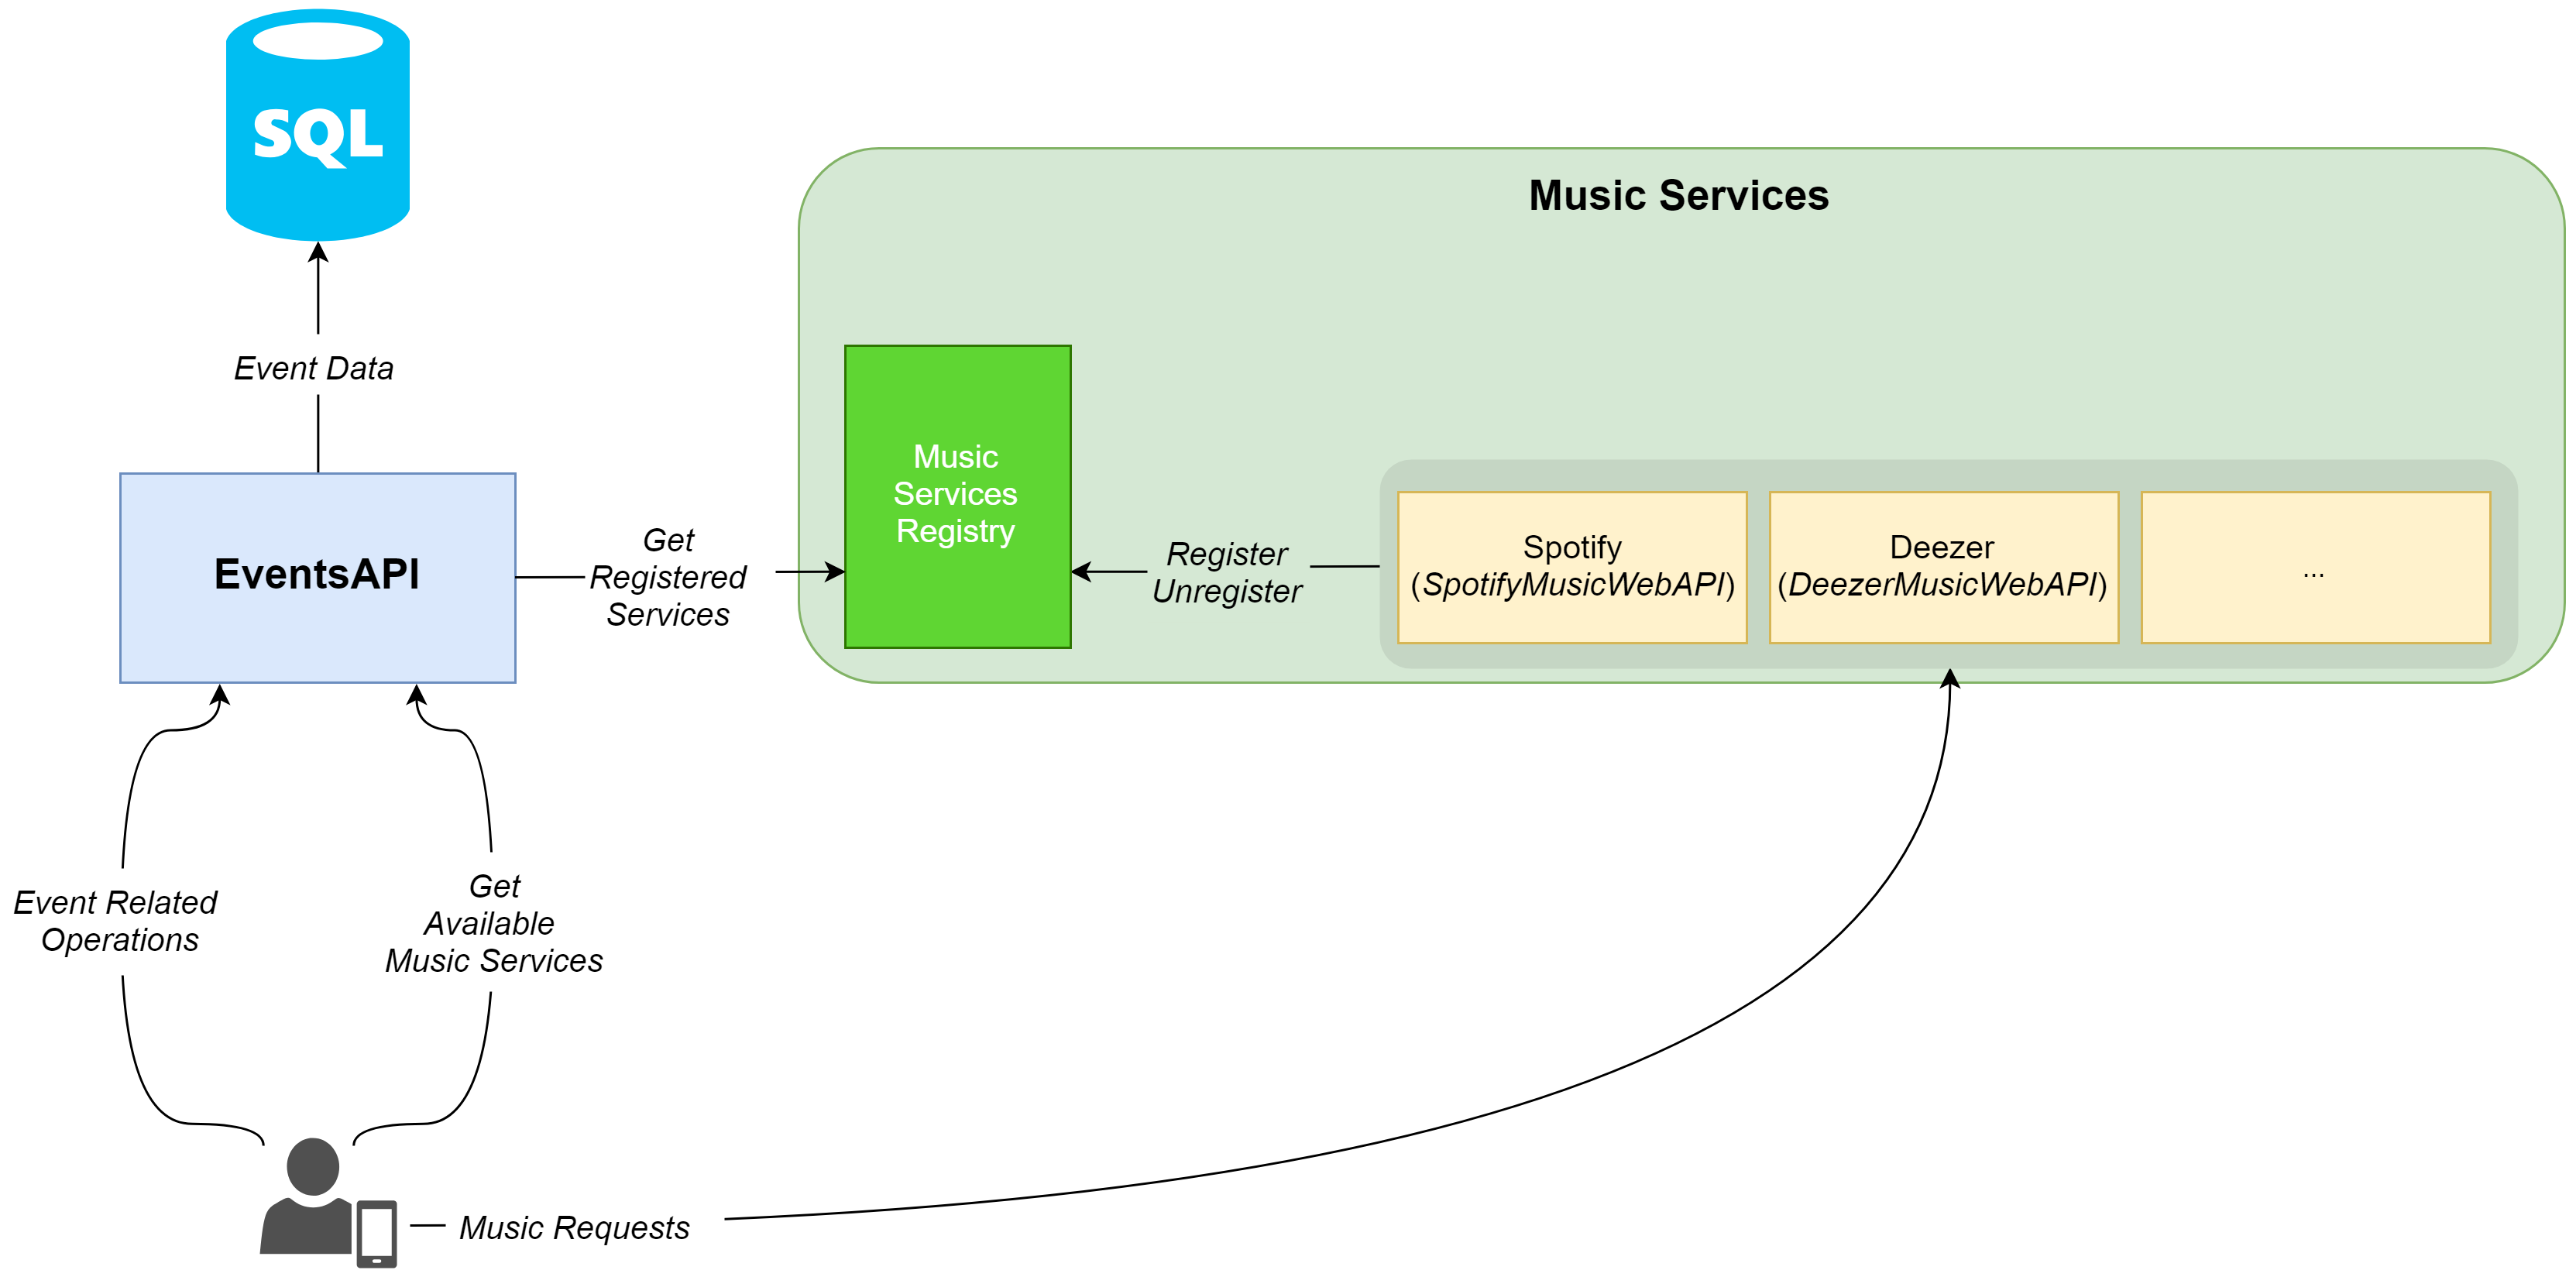
\includegraphics[width=0.75\textwidth]{./Chapter4/Figures/Architecture.png}
	\caption{System architecture.}
	\label{fig:SystemArchitecture}
\end{figure}

\subsection{Client}

The client component of this project is implemented as a mobile application, using the \textit{Android} and \textit{Windows} platform.

\subsection{Server}

The server component is implemented as a REST API, using .NET Core MVC.
\begin{itemize}	
	\item Event API - Supports the event creation and all of its operations (adding, editing and removing guests, expenses, tasks, among others);
	
	\item Music API - Supports the \textit{playlist} creation;
	
	\item Payments API (optional) - Supports the payment of the event's expenses.
	
\end{itemize}

The database operations are supported by the PostgreSQL database engine.

\subsubsection{Observations}

The motivation behind choosing this server-client architecture is the possibility of eventually creating other clients, without having to change the servers that support it.

The reason why the Payments and Media API aren't unified into the Event API is for the sake of having the benefit of the client only communicating with these APIs, yet having the possibility of comunicating with a wide range of services without having to implement them specifically.

The motivation behind the usage of SQL instead of NoSQL database types is because the entities used in this application are of relational types. Also, the atomicty and transactional behaviour that SQL databases support is of importance for consistency across event information.




%/////////////////////////////////////////////////////////////
%   Chapter 5
%
%    Timetabling
%
%/////////////////////////////////////////////////////////////

\chapter{HTR Model} 
\label{ch:Chapter5}
\vfill \minitoc \newpage

\section{Introduction}
Handwriting recognition \gls{htr} is a technology that converts handwritten text into digital format. Its purpose is to enable the efficient processing, storage, and manipulation of handwritten content through automated recognition algorithms.

\subsection{Offline HTR}
Offline handwriting recognition refers to the technology and process of converting static images or scans of handwritten text into digital text or characters. Unlike online handwriting recognition, which interprets handwriting in real time as it is being written, Offline \gls{htr} analyzes pre-existing images or documents that have been captured or scanned.

The goal of Offline \gls{htr} is to accurately recognize and convert the handwritten text in images into editable and searchable digital format. This technology finds applications in digitizing historical documents, handwritten notes, forms, and any other handwritten content that needs to be converted into machine-readable text.

The process of Offline \gls{htr} typically involves several steps:
\begin{itemize}
    \item Detection: In the detection phase, the handwritten text regions within the scanned or captured images are identified. This can be achieved through techniques such as text detection algorithms, connected component analysis, or contour-based methods. The goal is to localize and extract the regions containing the handwritten content for further processing.

    \item Image preprocessing: The scanned or captured images are enhanced, filtered, and prepared to optimize the quality of the handwriting for recognition. This may involve noise reduction, binarization, deskewing, and other techniques.
    
    \item Recognition: Machine learning algorithms, such as neural networks or Hidden Markov Models (HMM), are trained using labeled samples of handwritten characters or words. These models are then used to recognize and classify the extracted features into corresponding textual representations.

    \item Post-processing: The recognized text is further refined and processed to improve accuracy, correct errors, handle ambiguities, and align with language-specific rules and dictionaries.

\end{itemize}


\subsection{Online HTR}
Online handwriting recognition refers to the technology and process of converting handwritten input into digital text or characters in real time. It involves capturing and interpreting the movements and patterns made by a user while writing using a stylus or a digital pen on a touch-enabled device, such as a tablet or a smartphone.

Unlike offline handwriting recognition, which analyzes static images of handwritten text, online handwriting recognition takes advantage of the temporal information obtained during the writing process. This allows for real-time interpretation and immediate feedback as the user writes, making it suitable for applications where instant recognition is required, such as note-taking, electronic signature verification, form filling, and interactive whiteboards.

Online handwriting \textit{\cite{OnlineHTR}} recognition systems typically use various techniques, including pattern recognition algorithms, machine learning, and neural networks, to analyze the dynamic information provided by the user's pen strokes. These algorithms analyze factors such as stroke speed, direction, pressure, and sequence to identify and interpret the handwritten characters or gestures. The recognized text can then be further processed, stored, or used in various applications and systems that require digital text input.


\section{Implementation}
In this section we will talk about the decisions made and explain the implementation of each component.
\subsection{Why Offline HTR}
In a project like this, it initially seems like a no-brainer to implement Online \gls{htr} instead of Offline \gls{htr}. However, the lack of complex yet comprehensive documentation for beginners pose a significant roadblock. Without readily available resources and clear guidance, the implementation process becomes more complex and time-consuming. This led to frustration and delays as the we struggled to navigate the complexities of Online \gls{htr} without proper guidance.

Furthermore, the absence of open-source implementations of Online \gls{htr} hinders collaboration and knowledge sharing within the community. Open-source projects often serve as valuable starting points, providing code samples, libraries, and frameworks that accelerate the development process. Without such resources, we must start from scratch or rely on proprietary solutions, limiting the ability to customize and adapt the \gls{htr} system to the specific project requirements. The potential benefits of enhanced accuracy,  real time text recognition, and dynamic input support opportunities may be overshadowed by the steep learning curve and lack of accessible resources for offline \gls{htr} implementation.

As a result, the decision to implement Offline \gls{htr} becomes less straightforward yet possible thanks to widely available open-source implementations and good guidance examples such as the one followed to implement our model \textit{\cite{HTR}}.


\subsection{Pipeline}
The \gls{htr} system follows a pipeline-based approach to process images and extract text. The pipeline consists of two main stages: text detection and text recognition.
The Figure~\ref{fig:HTRS} represents a overview of the implemented \gls{htr} system. For our needs it takes a PNG containing the postcard drawn content and returns the text as a String. 

\begin{figure}[!ht]
	\centering
	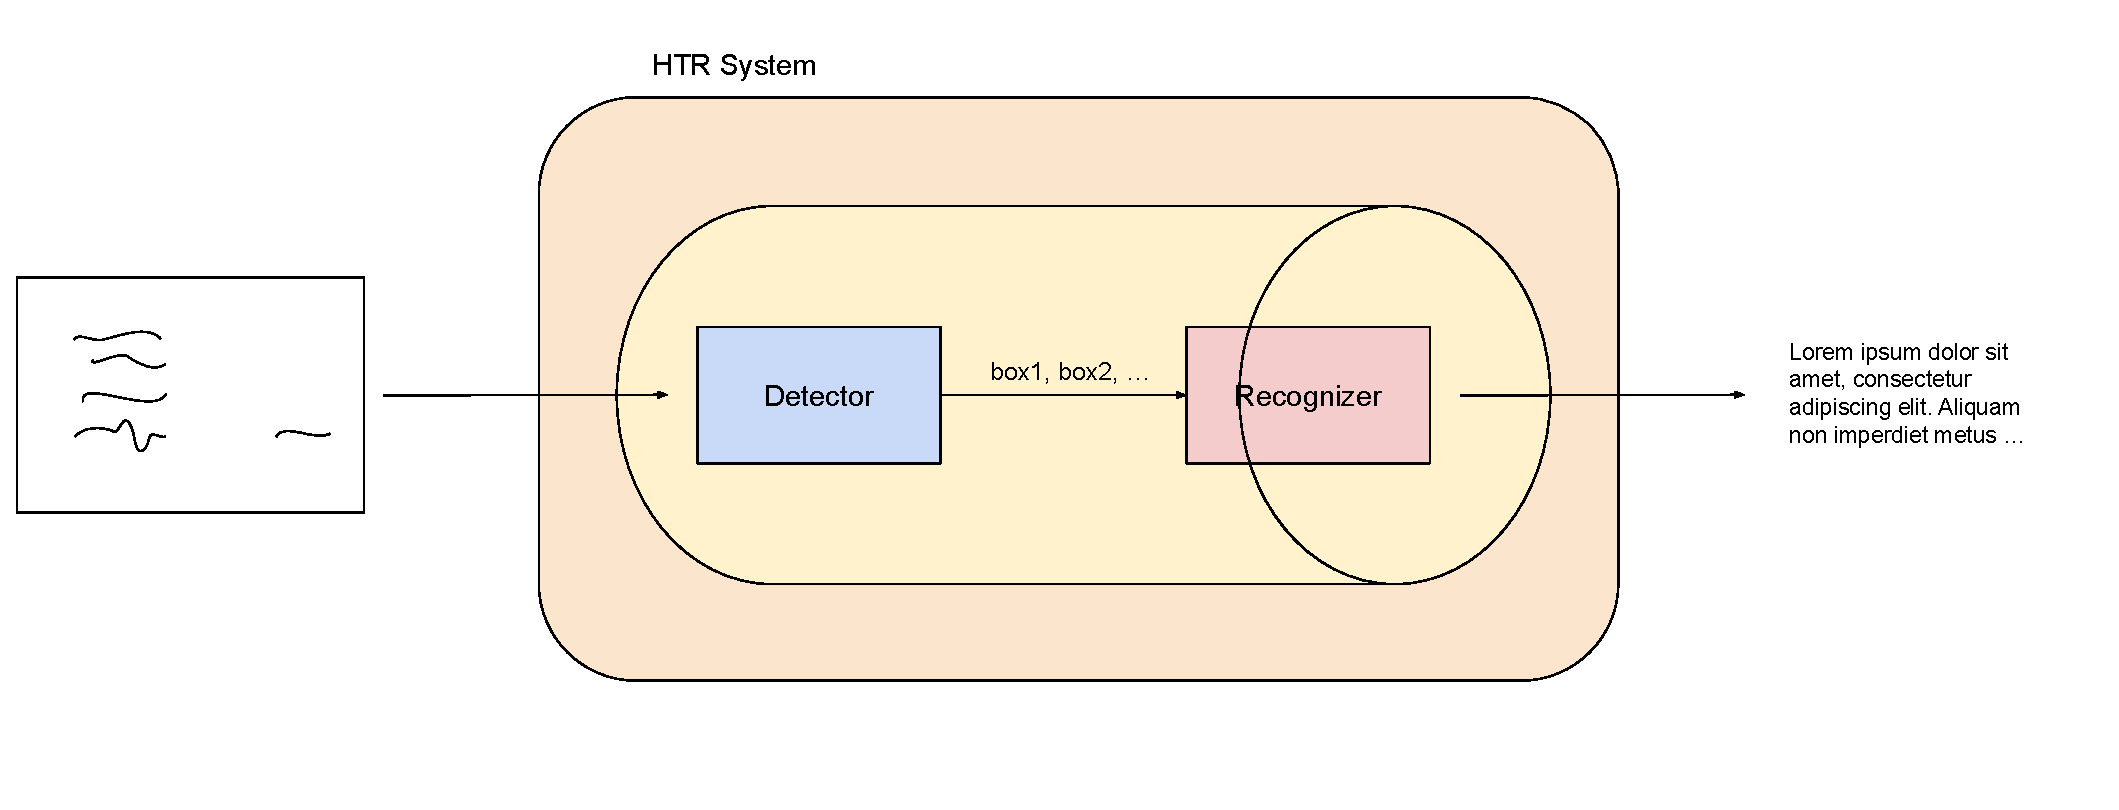
\includegraphics[trim={ 0.2cm 1cm 0cm 0cm },width=1\textwidth]{./Chapter5/Figures/HTR System}
	\caption{HTR System}
	\label{fig:HTRS}
\end{figure}

\textbf{Both components use the Tensorflow framework and are written in python.}

\subsection{Detector}
The detection is made possible by using CRAFT-Text \textit{\cite{CRAFT-Text}} detection implementation from \textit{\cite{Keras-ocr}}. The particular detector was trained for machine-generated characters based on fonts but still manages to give good results for handwritten text, big part of it's good results is the absence of visual clutter in the background as we only provide the drawn content to the model. 


The Figure~\ref{fig:Detector} illustrates how the detector works, keeping in mind that the figure is simplified for explanatory purposes and the detector detects words and not lines.

\begin{figure}[!ht]
	\centering
	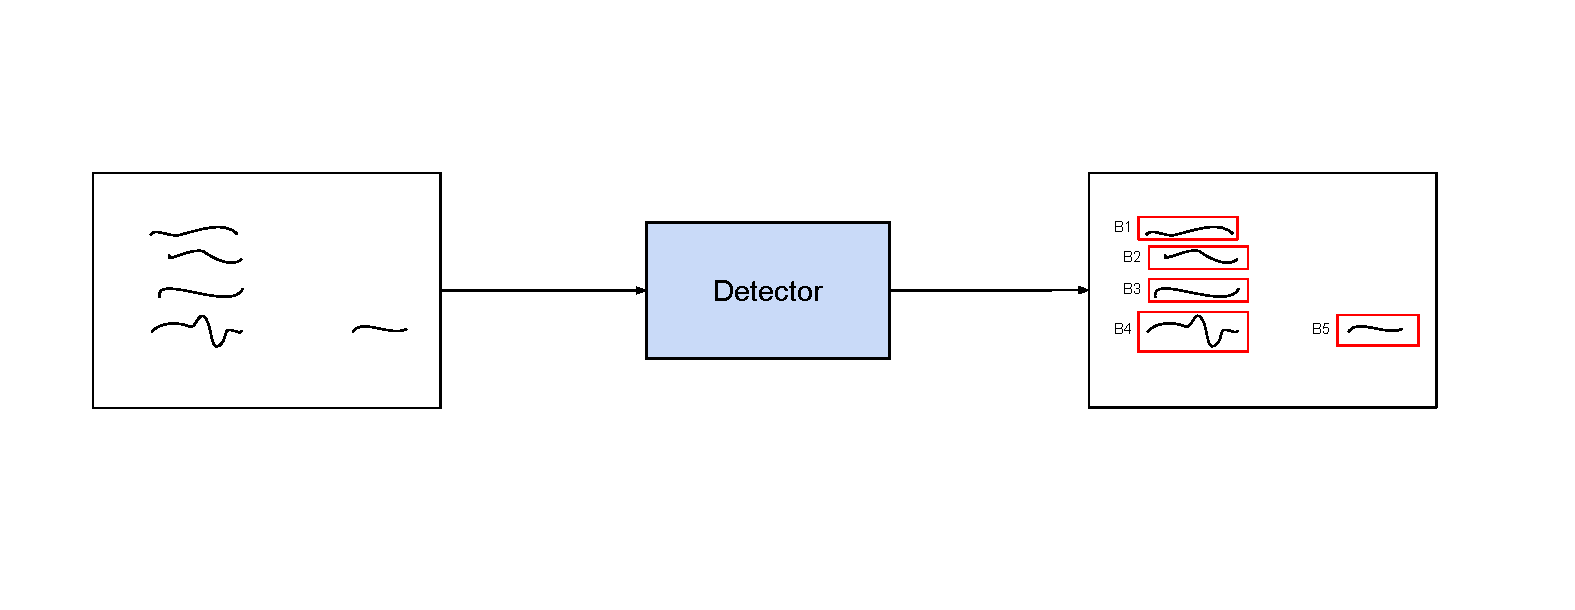
\includegraphics[trim={2cm 3cm 0 1cm}, width=1.1\textwidth]{./Chapter5/Figures/Detector}
	\caption{Detection Flow}
	\label{fig:Detector}
\end{figure}

The returned value from the detector model is a list containing four points (x and y) defining a box that represents where the word is relative to the image.


\subsection{Recognizer}
The text recognition stage takes the boxes from the detector and processes them to extract the actual text content creating a temporary file for each box. It applies character segmentation, feature extraction, and sequence modeling techniques to recognize and convert the text regions into machine-readable format. A layer by layer summary based on online documentation:
\begin{itemize}
    \item Input Layer: The model takes an input image with dimensions (128, 32, 1), representing a grayscale image. It also takes input labels, which are sequences of characters.
    \item Convolutional Layers: The model starts with two convolutional blocks. Each block consists of a 2D convolutional layer followed by a max-pooling layer. The convolutional layers learn local image features and the max-pooling layers downsample the feature maps.
    \item Reshaping and Dense Layer: After the convolutional layers, the feature maps are reshaped to a new shape that is compatible with the recurrent part of the model. This reshaping operation prepares the data for input to the recurrent layers. The reshaped features pass through a fully connected dense layer with 64 units and ReLU activation.
    \item Dropout Regularization: A dropout layer is applied to reduce overfitting by randomly setting a fraction of the input units to 0 during training.
    \item Recurrent Layers: Two bidirectional LSTM layers are stacked on top of each other. Bidirectional LSTMs process the input sequence in both forward and backward directions, allowing the model to capture dependencies in both directions. The LSTM layers have dropout applied to them to prevent overfitting.
    \item Output Layer: A dense layer with a softmax activation is used as the output layer. The number of units in this layer corresponds to the vocabulary size (number of characters) plus two special tokens introduced by the CTC loss. The softmax activation produces a probability distribution over the characters.
    \item CTC Loss Layer: The output of the softmax layer is passed to the Connectionist Temporal Classification (CTC) layer. The CTC layer calculates the CTC loss, which measures the difference between the predicted sequence and the ground truth labels. It takes both the labels and the output of the softmax layer as inputs.
    \item Model Compilation: The model is compiled with the Adam optimizer. The specific learning rate and other optimizer parameters can be further customized if needed.
    \item Model Output: The output of the model is the output of the CTC layer, representing the CTC loss. 

\end{itemize}


\begin{figure}[!ht]
	\centering
	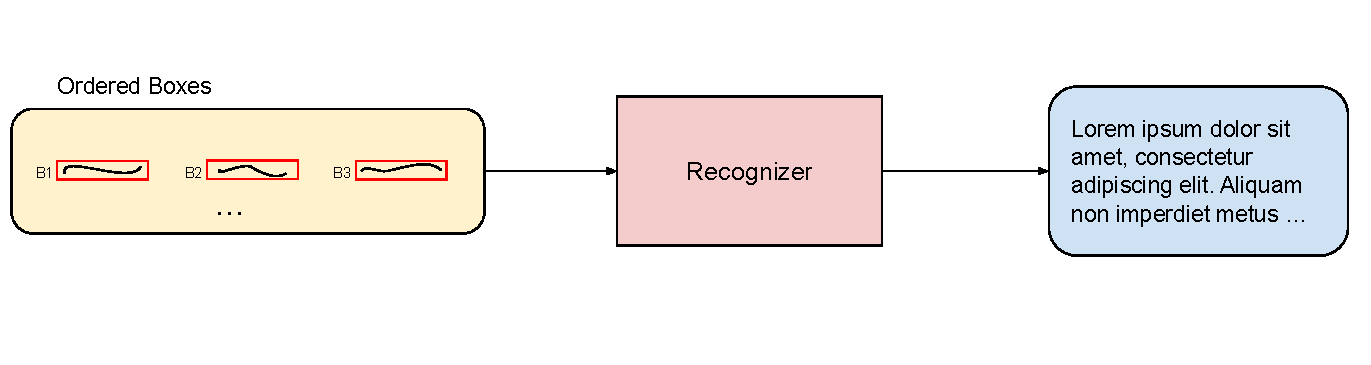
\includegraphics[trim={0cm 0cm 0 0cm}, width=1\textwidth]{./Chapter5/Figures/Recognizer}
	\caption{Recognizer Flow}
	\label{fig:Recognizer}
\end{figure}




\subsubsection{Image Preprocessing}
Image preprocessing is a critical step in offline \gls{htr} systems as it aims to enhance the quality of scanned or captured handwritten images before they are fed into the recognition model. The objective is to optimize the images for accurate recognition by applying various transformations and adjustments.

In the context of our project, the provided code snippet offers a foundational approach to image preprocessing.

Reading and Decoding Image:

The first step involves reading the image file using tf.io.read\_file and decoding it using tf.image.decode\_png.
By decoding the image as grayscale (decode\_png(image, 1)), we ensure that only the necessary information is retained.
Distortion-Free Resizing:

To achieve consistent input sizes, the distortion\_free\_resize function is employed for resizing the image to the desired dimensions (img\_size).
During resizing, the preserve\_aspect\_ratio=True parameter ensures that the original aspect ratio of the image is maintained.
This function intelligently pads the image symmetrically to ensure uniformity and prevent distortion.
Normalization:

After resizing, the image is cast to tf.float32 and normalized to a range between 0 and 1 by dividing each pixel value by 255.0.
Normalization facilitates improved convergence during training and enhances the overall performance of the recognition model.
By utilizing the preprocess\_image function, we establish a solid foundation for handling image preprocessing in our offline \gls{htr} system. This function accepts an image path as input and performs resizing, padding, and normalization operations to prepare the image for subsequent processing.


\subsubsection{Training}
The recognizer was trained using the \textit{\cite{IAM}} words dataset, which is a widely used benchmark dataset for \gls{htr} research. The IAM dataset is a comprehensive collection of handwritten English text samples contributed by different writers. It consists of 86810 training samples, 4823 validation samples and 
4823 test samples.

To get good results the recognizer was trained for roughly 60 iterations in Google's Colab Notebook servers.

\paragraph{Tweaks}
After each training iteration, the Tensorflow training process incorporates additional code through callbacks to enhance its functionality. In this particular scenario, two tweaks have been added to optimize the training process:
\begin{itemize}
    \item Early Stopping Callback:
    An early stopping callback is implemented to monitor the model's performance during training and determine if it is not improving.
    The patience parameter is set to 3, indicating that if the model does not show improvement for 3 consecutive iterations, the training process will stop early.
    By setting restore\_best\_weights to True, the callback ensures that the best weights achieved during training are restored before stopping, allowing for optimal model performance.
    The verbose parameter is set to 1, enabling the callback to display informative messages about its operations. 
    \item Checkpoint Callback:
    A checkpoint callback is added to periodically save the model's weights during training.
    The filepath parameter specifies the path where the weights will be saved.
    By setting save\_weights\_only to True, only the weights of the model will be saved, reducing storage requirements.
    The verbose parameter is set to 1, enabling the callback to display informative messages about the saving process.
\end{itemize}

These tweaks improve the training process by introducing early stopping criteria based on the model's performance and by providing checkpoints to save the model's weights at different stages.


\subsubsection{Postprocessing}
To be able to decode the output produced by the Output Layer (dense 2) a function called  \textit{decode\_batch\_predictions} is implemented in the guide \textit{\cite{HTR}}.

The function takes the model predictions pred as input. These predictions are usually in the form of probability distributions over the characters in the vocabulary for each time step.

The variable input\_len is created to specify the length of the input sequences for each prediction in the batch. It is set to be the same for all predictions and is equal to the number of time steps in the predictions.

The function utilizes the CTC (Connectionist Temporal Classification) decoding method to convert the predictions into sequences of characters. It applies the ctc\_decode function from Keras backend, passing the predictions, input length, and using greedy search (other methods like beam search can be used for more complex tasks). The ctc\_decode function returns the decoded sequences.

The results variable stores the decoded sequences. It selects the first element [0][0] from the ctc\_decode output, which represents the decoded labels for the batch. It also truncates the sequences to a maximum length max\_len if necessary.

The function iterates over each decoded sequence in results. For each sequence, it applies several operations to convert the numerical labels to actual text.

First, it uses tf.where to find the positions where the labels are not equal to -1 (a special token often used in CTC decoding to represent blank or no label).

It then uses tf.gather to gather the non-equal elements from the labels.

The gathered labels are passed through num\_to\_char function, which maps the numerical labels to their corresponding characters.

Next, tf.strings.reduce\_join is applied to concatenate the characters into a single string representation.

Finally, numpy().decode("utf-8") is used to convert the string from a TensorFlow tensor to a regular Python string, and the resulting string is appended to the output\_text list.

After iterating over all the sequences in results, the function returns the output\_text list, which contains the decoded texts for each prediction in the batch.

In summary, the decode\_batch\_predictions function takes the model predictions, performs CTC decoding to convert the predictions into sequences of characters, and applies additional post-processing steps to obtain the final text representations for the predictions.


\subsection{Natural Text Ordering}
One of the challenges in \gls{htr} is maintaining the natural ordering of text when dealing with multi-line or multi-column documents. To address this challenge, we came up with a algorithm that uses the average box size to calculate a margin of error for each point in a line.
In our implementation there is always two fixed boxes Figure~\ref{fig:PFBoxes}

\begin{figure}[!ht]
	\centering
	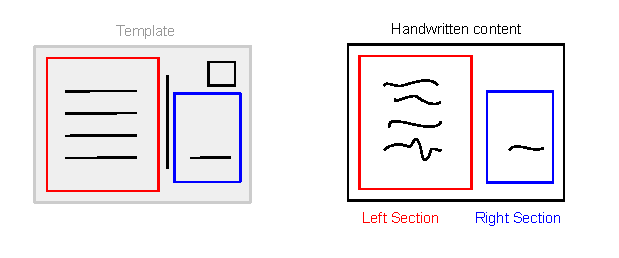
\includegraphics[trim={0cm 0cm 0 0cm}, width=1\textwidth]{./Chapter5/Figures/Main Sections Postcard}
	\caption{Postcard Main Sections}
	\label{fig:PFBoxes}
\end{figure}

\newpage

The ordering algorithm works like this:

We start by calculating the height of every box, using vector calculation. We do this for every box and divide by the number of boxes obtaining the average box height.

\begin{figure}[!ht]
	\centering
	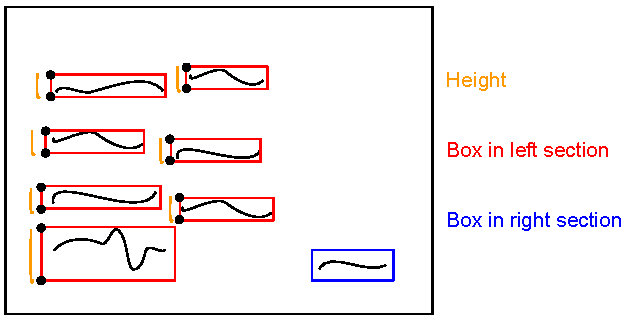
\includegraphics[trim={0cm -0.5cm 0 -0.5cm}, width=0.7\textwidth]{./Chapter5/Figures/Height Box}
	\caption{Average height calculation for left section}
	\label{fig:AVGH}
\end{figure}


Now all we have to do is pick the same located point in every box (top left or right left, etc...) and test the y value +- the calculated average box/2. If the y value is inside the range y-average height/2 to y+average height/2 then compare the x values else compare the y values. A lower x value means it comes earlier in the natural ordering. A higher y value than the current one means it comes later in the natural ordering. 

\section{Limitations}
IAM dataset vocabulary is primarily focused on the English language. It includes a wide range of alphanumeric characters, including uppercase and lowercase letters (A-Z, a-z), digits (0-9), and common punctuation marks. However, it does not cover the entire spectrum of possible characters that can exist in different languages or writing systems.

This vocabulary limitation means that the IAM dataset may not be suitable for recognizing text in languages other than English or for dealing with specialized symbols or characters that are outside the dataset's predefined set. For example, if the dataset does not include characters specific to a particular language or domain, the \gls{htr} model trained on IAM may struggle to accurately recognize and transcribe such characters.

While having made all the possible optimizations for using the detector, if the user draws text right next to each other there's a good change it will detect it all as a whole word.

\section{Results}
Results tend to vary a lot depending on the input image. 

Thicker line strokes, angled letters and image quality are some of the factors that directly influence the final output.

Higher quality images (more pixels) and thinner stroke lines tend to get better results.

These are the obtained results:
\begin{itemize}
	\item Figure~\ref{fig:T1} - Thiss is a tost image with arial font Hollo MHTPR model
	\item Figure~\ref{fig:T2} - Heito Worild Thiss is a HT. modet DoRs It works Antonio Canvatho
	\item Figure~\ref{fig:T3} - This is a tost Mello world Can you read thist 
	\item Figure~\ref{fig:T4} - this is a Tasst
\end{itemize} 

\begin{figure}[!ht]
	\centering
	\fbox{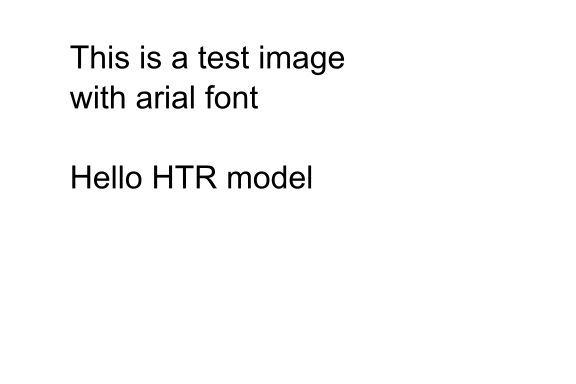
\includegraphics[trim={0cm -0.5cm 0 -0.5cm}, width=0.7\textwidth]{./Chapter5/Figures/test1}}
	\caption{Test figure 1}
	\label{fig:T1}
\end{figure}

\begin{figure}[!ht]
	\centering
	\fbox{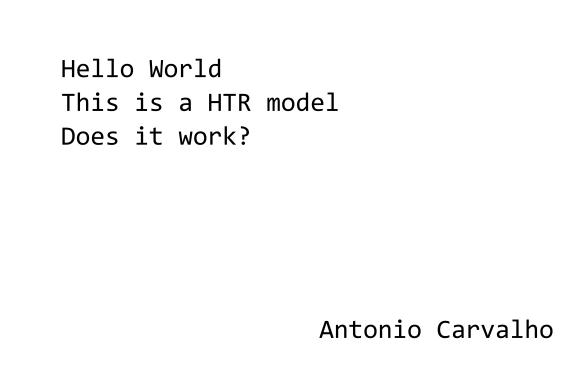
\includegraphics[trim={0cm -0.5cm 0 -0.5cm}, width=0.7\textwidth]{./Chapter5/Figures/test2}}
	\caption{Test figure 2}
	\label{fig:T2}
\end{figure}


\begin{figure}[!ht]
	\centering
	\fbox{
\includegraphics[trim={0cm -0.5cm 0 -0.5cm}, width=0.7\textwidth]{./Chapter5/Figures/test3}}
	\caption{Test figure 3}
	\label{fig:T3}
\end{figure}


\begin{figure}[!ht]
	\centering
	\fbox{
\includegraphics[trim={0cm -0.5cm 0 -0.5cm}, width=0.7\textwidth]{./Chapter5/Figures/test4}}
	\caption{Test figure 4}
	\label{fig:T4}
\end{figure}






%/////////////////////////////////////////////////////////////
%   Chapter 6
%
%   
%
%/////////////////////////////////////////////////////////////
%\chapter{Client} 
\label{ch:Chapter6}
\vfill \minitoc \newpage

The client was implemented in Android and uses Android's Jetpack Compose UI toolkit.

\begin{figure}[!ht]
	\centering
	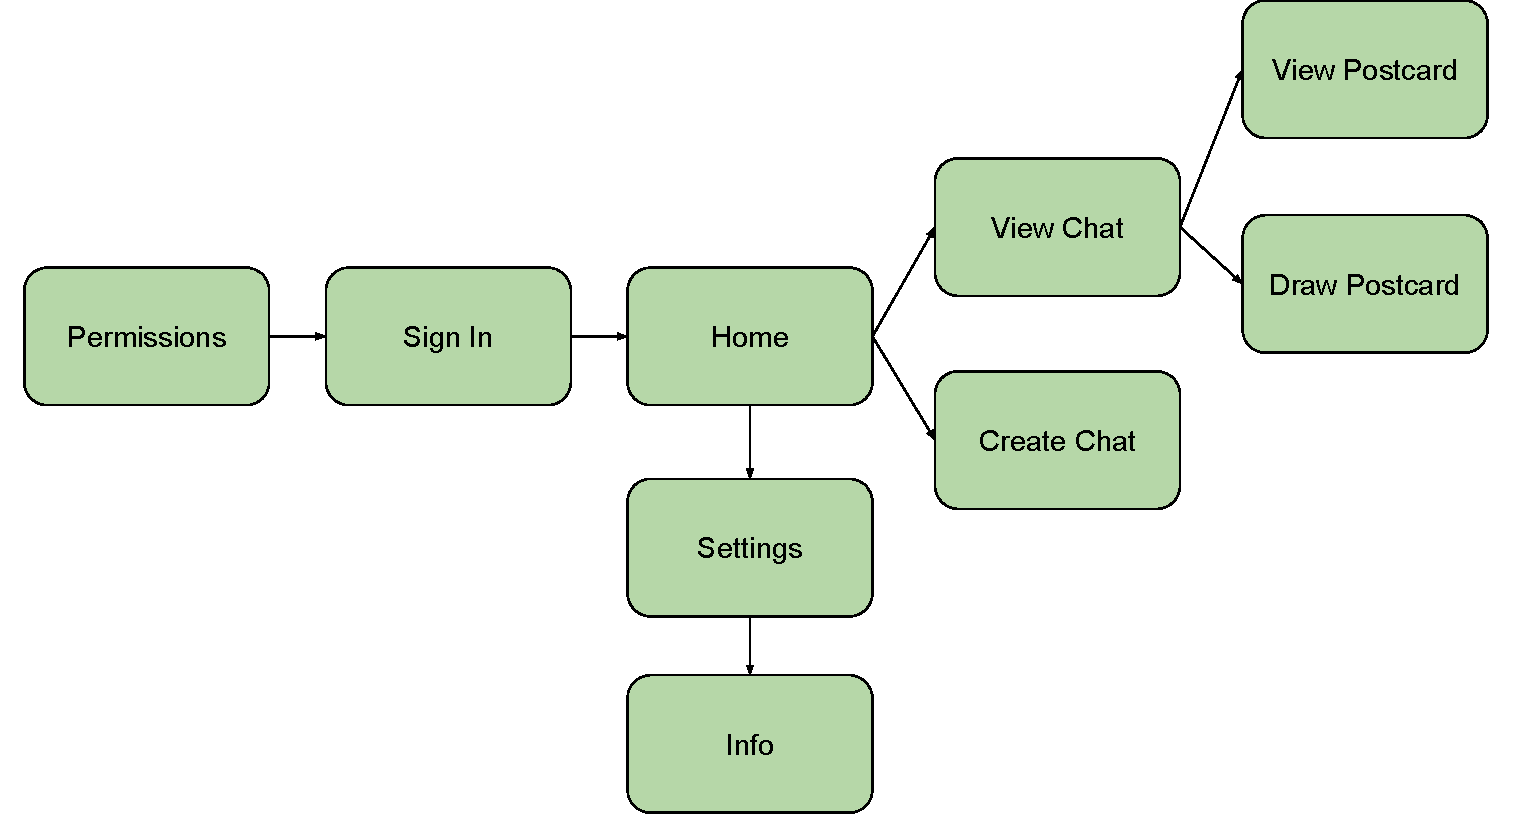
\includegraphics[trim={0cm 0cm 0 0cm}, width=1\textwidth]{./Chapter6/Figures/Android NavGraph}
	\caption{Android Activity Navigation Graphic}
	\label{fig:NavgGraph}
\end{figure}


\section{Android System and Compose Framework Overview}
Before showing the client implementation its best to give some context and basic knowledge about the android system and the Compose framework.

\subsection{Android Manifest}
The AndroidManifest.xml file is an essential configuration file in Android development that provides essential information about the Android application to the Android system. It is located in the root directory of the Android project and is required for every Android application.

The Android manifest file contains important metadata about the app, including its package name, version number, permissions, activities, services, broadcast receivers, and more. It serves as a blueprint for the Android system to understand the structure and behavior of the application.

\subsection{Android Activity}
In the context of Android app development, an Activity is a fundamental component of an Android application that represents a single screen with a user interface. It is a crucial part of the overall app architecture and is responsible for handling user interactions and presenting visual elements to the user.

An Activity acts as a container for the user interface and provides a window in which the app's UI elements, such as buttons, text fields, images, and other widgets, are displayed. It manages the lifecycle of these UI components and handles user input events, such as button clicks or touch gestures.

Each Activity has a corresponding Java or Kotlin class that extends the Activity base class or its subclasses provided by the Android framework. This class contains methods that define the behavior of the Activity during different stages of its lifecycle, such as creation, starting, pausing, resuming, stopping, and destruction.

When an app is launched, typically, the main Activity is created and displayed to the user. The Activity is responsible for setting up the initial UI layout, interacting with data sources (e.g., retrieving data from a database or an API), and responding to user actions. It can also communicate with other Activities, such as starting a new Activity for a different screen or receiving results from a previously started Activity.

\subsection{Data Storing}
Android uses a file system that's similar to disk-based file systems on other platforms. The system provides several options for you to save your app data:
\begin{itemize}
    \item App-specific storage: Store files that are meant for your app's use only, either in dedicated directories within an internal storage volume or different dedicated directories within external storage. Use the directories within internal storage to save sensitive information that other apps shouldn't access;
    \item Shared storage: Store files that your app intends to share with other apps, including media, documents, and other files;
    \item Preferences: Store private, primitive data in key-value pairs;
    \item Databases: Store structured data in a private database using the Room persistence library.    
\end{itemize}


\subsection{ViewModel}
The ViewModel class is a business logic or screen level state holder. It exposes state to the UI and encapsulates related business logic. Its principal advantage is that it caches state and persists it through configuration changes. This means that your UI doesn’t have to fetch data again when navigating between activities, or following configuration changes, such as when rotating the screen.

\subsection{Canvas}
The Android Canvas is a fundamental graphics component provided by the Android framework. It serves as a drawing surface onto which we can render custom graphics, shapes, images, and text. The Canvas provides a set of drawing methods that allow us to create and manipulate visual elements within an Android application.

When working with the Canvas, we can perform various operations such as drawing lines, rectangles, circles, arcs, and paths. We can also apply transformations like translation, rotation, scaling, and skewing to manipulate the position and orientation of the drawn elements. Additionally, the Canvas supports the rendering of text, allowing us to display custom text with different fonts, sizes, colors, and styles.

\subsection{Making HTTP Request}
When developing Android applications, it is common to interact with web services and APIs to retrieve data or send data to a server. One popular library for making HTTP requests in Android is OkHttp.

\subsubsection{OkHttp}
OkHttp is an open-source HTTP client library for Java and Android applications. It is developed by the same team behind the widely-used Retrofit library and offers a simple and efficient way to make HTTP requests and handle responses. OkHttp is built on top of the Java standard library's HttpURLConnection, providing a more convenient and powerful API.


\section{Activities}
In this section we will demonstrate all activities implemented.
\subsection{Permissions}
The Permissions activity handles all requests to permissions needed for the application to work.
The Application needs permission to read contacts.

Figures \ref{fig:PA} illustrates the implemented activity. 

\begin{figure}[!ht]
	\centering
	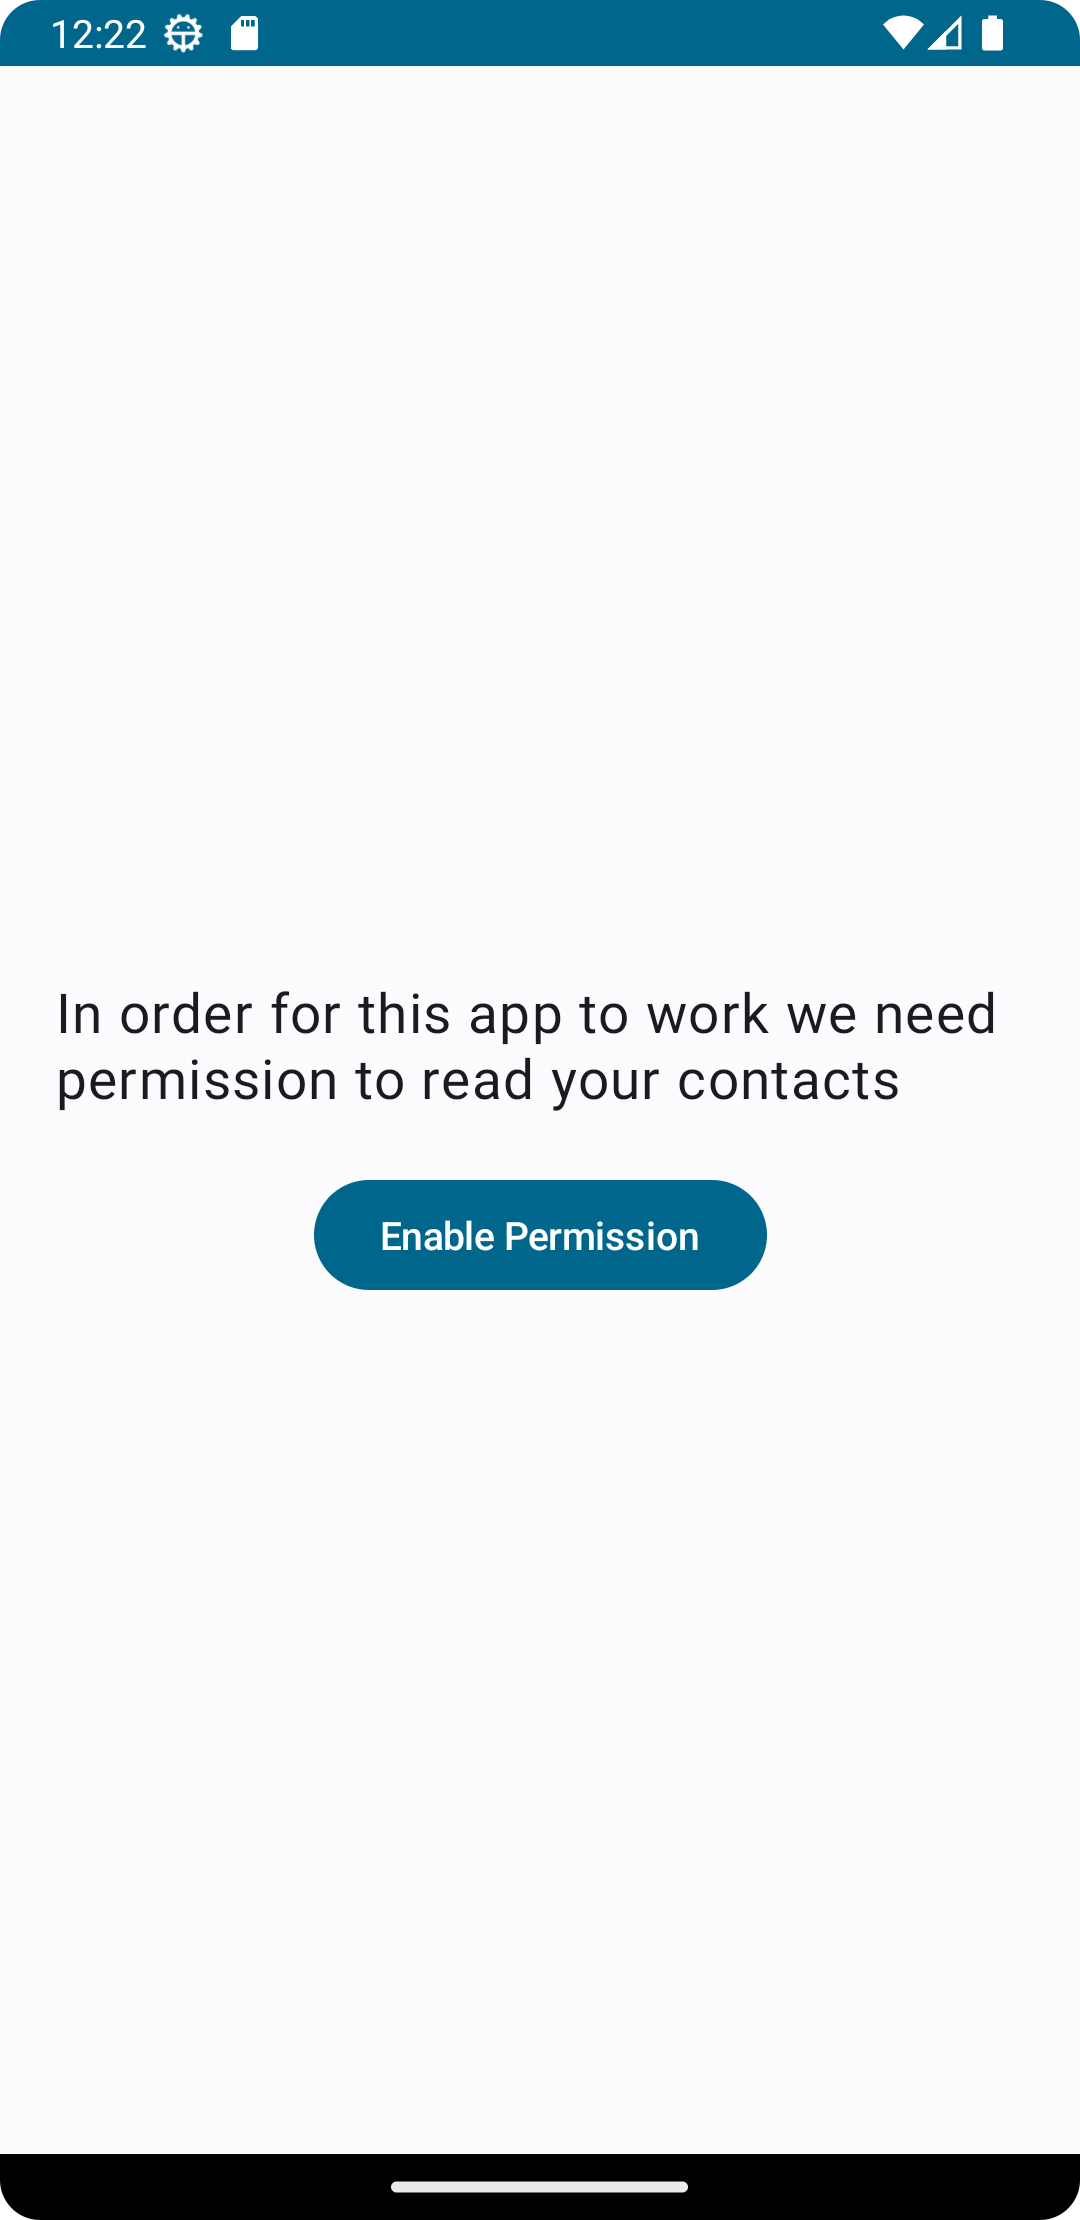
\includegraphics[trim={0cm 0cm 0 0cm}, width=0.4\textwidth]{./Chapter6/Figures/PermissionActivity}
	\caption{Permission Activity}
	\label{fig:PA}
\end{figure}


\subsection{Sign In}

The Sign-in Activity serves as the component for managing the user's authentication process, containing both logging in and registering in the service. Additionally, it ensures the secure storage of the user's token by leveraging the EncryptedSharedPreferences.

Upon launching the Sign-in Activity, users are presented with a user-friendly interface where they can enter their credentials or choose to register as a new user. The activity handles the input validation and securely communicates with the server-side authentication API.

Once the user's credentials are verified, the Sign-in Activity retrieves the authentication token from the server's response. To ensure the token's confidentiality, it is stored using the EncryptedSharedPreferences. This specialized SharedPreferences implementation employs encryption algorithms to protect sensitive data from unauthorized access.

By utilizing the EncryptedSharedPreferences, the Sign-in Activity safeguards the user's authentication token, preventing it from being tampered with or exposed. This secure storage mechanism provides an additional layer of protection for user data, mitigating the risks associated with unauthorized token access.


In addition, the Sign-in Activity incorporates an automatic phone number region retrieval feature by leveraging the Carrier information.

Because our app hasn't been deployed anywhere it is prompted to the user to choose whether he wants to use local data "Mock" or connect to an IP address - see \ref{SAIP}

Figures \ref{fig:SA1}, \ref{fig:SA2} illustrate the implemented activity.

\begin{figure}[!ht]
	\centering
	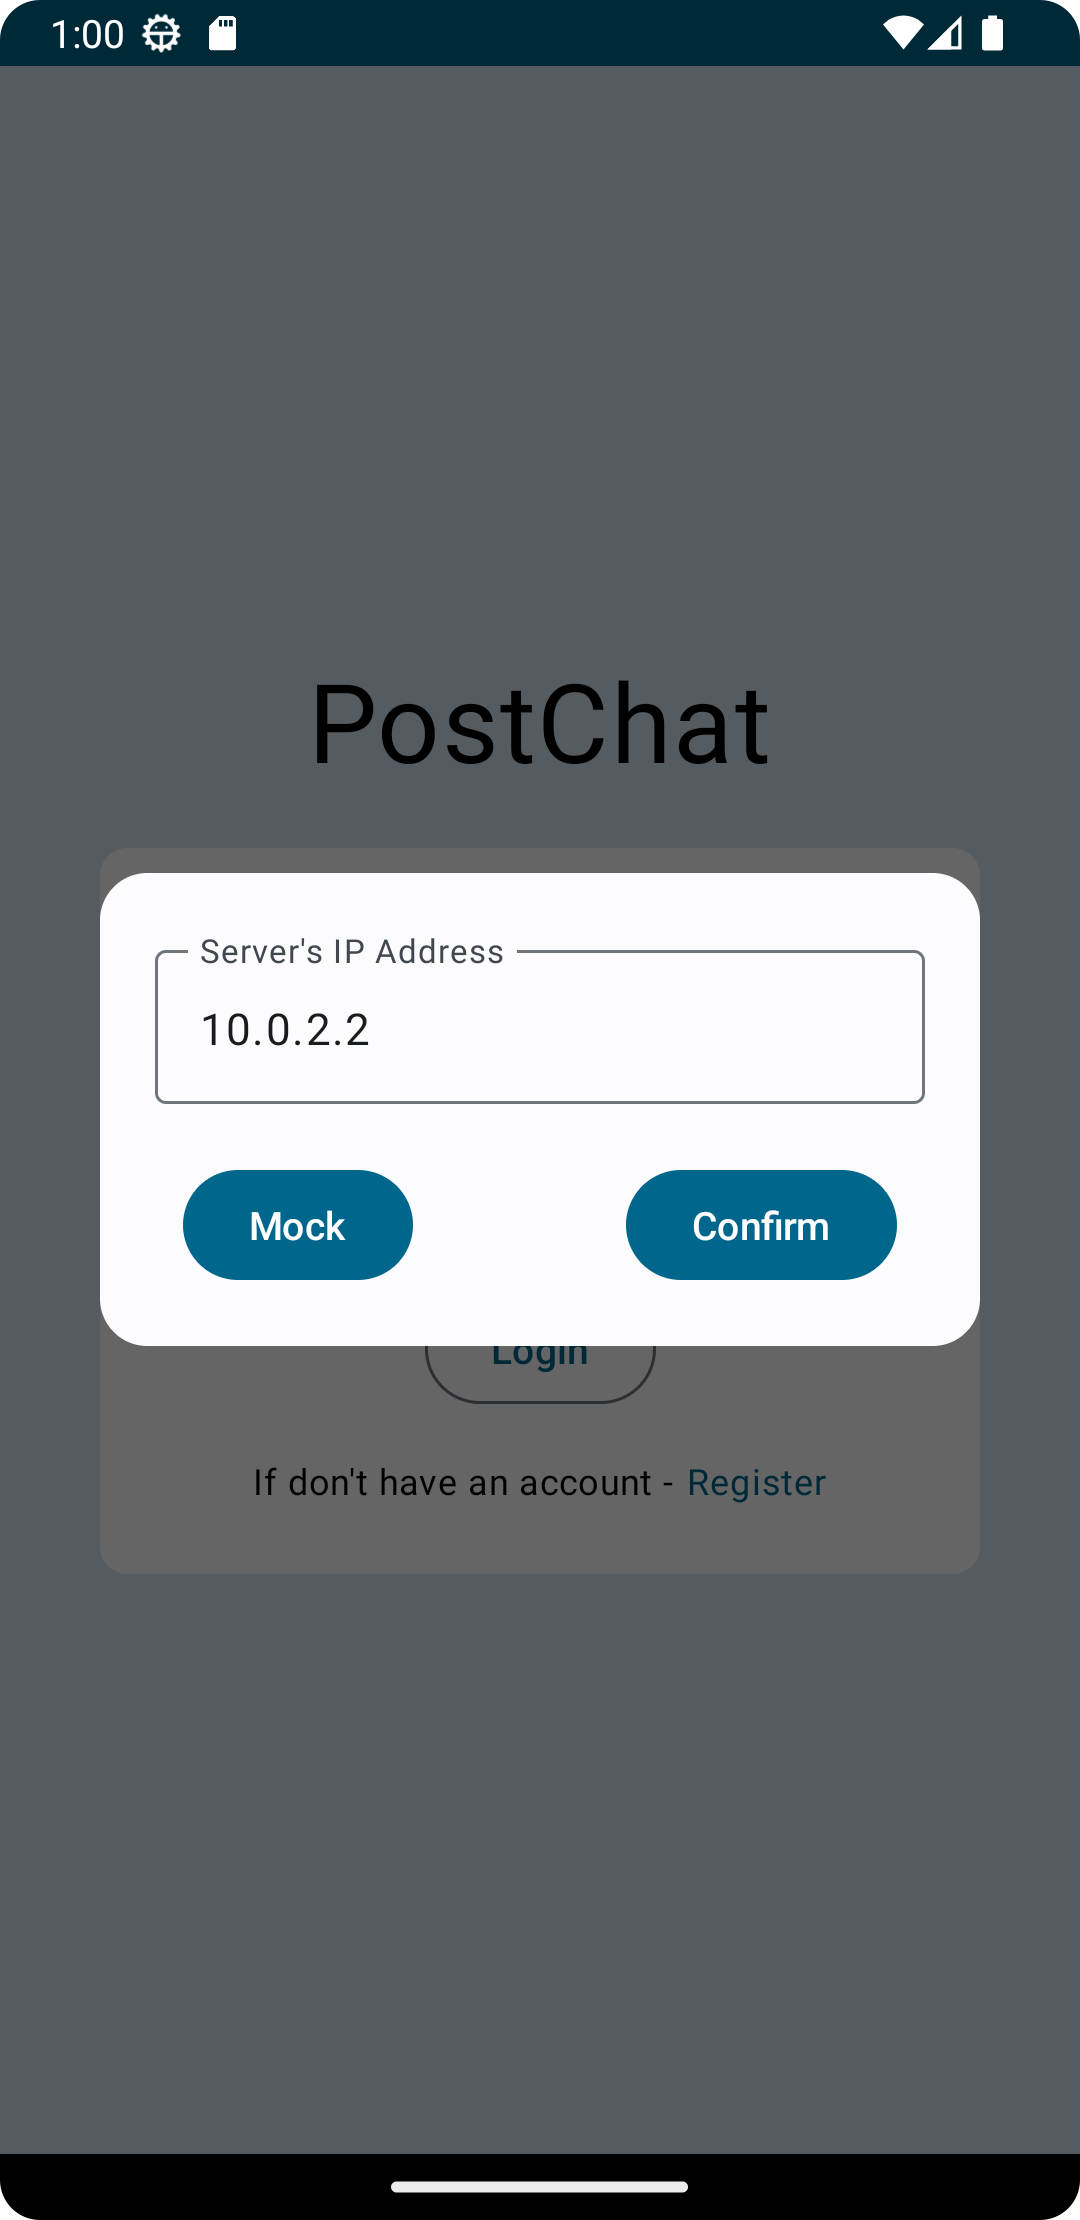
\includegraphics[trim={0cm -3cm 0 -3cm}, width=0.4\textwidth]{./Chapter6/Figures/SignInActivityIpAdress}
	\caption{Signin Activity}
	\label{fig:SAIP}
\end{figure}


\begin{figure}[!ht]
	\centering
	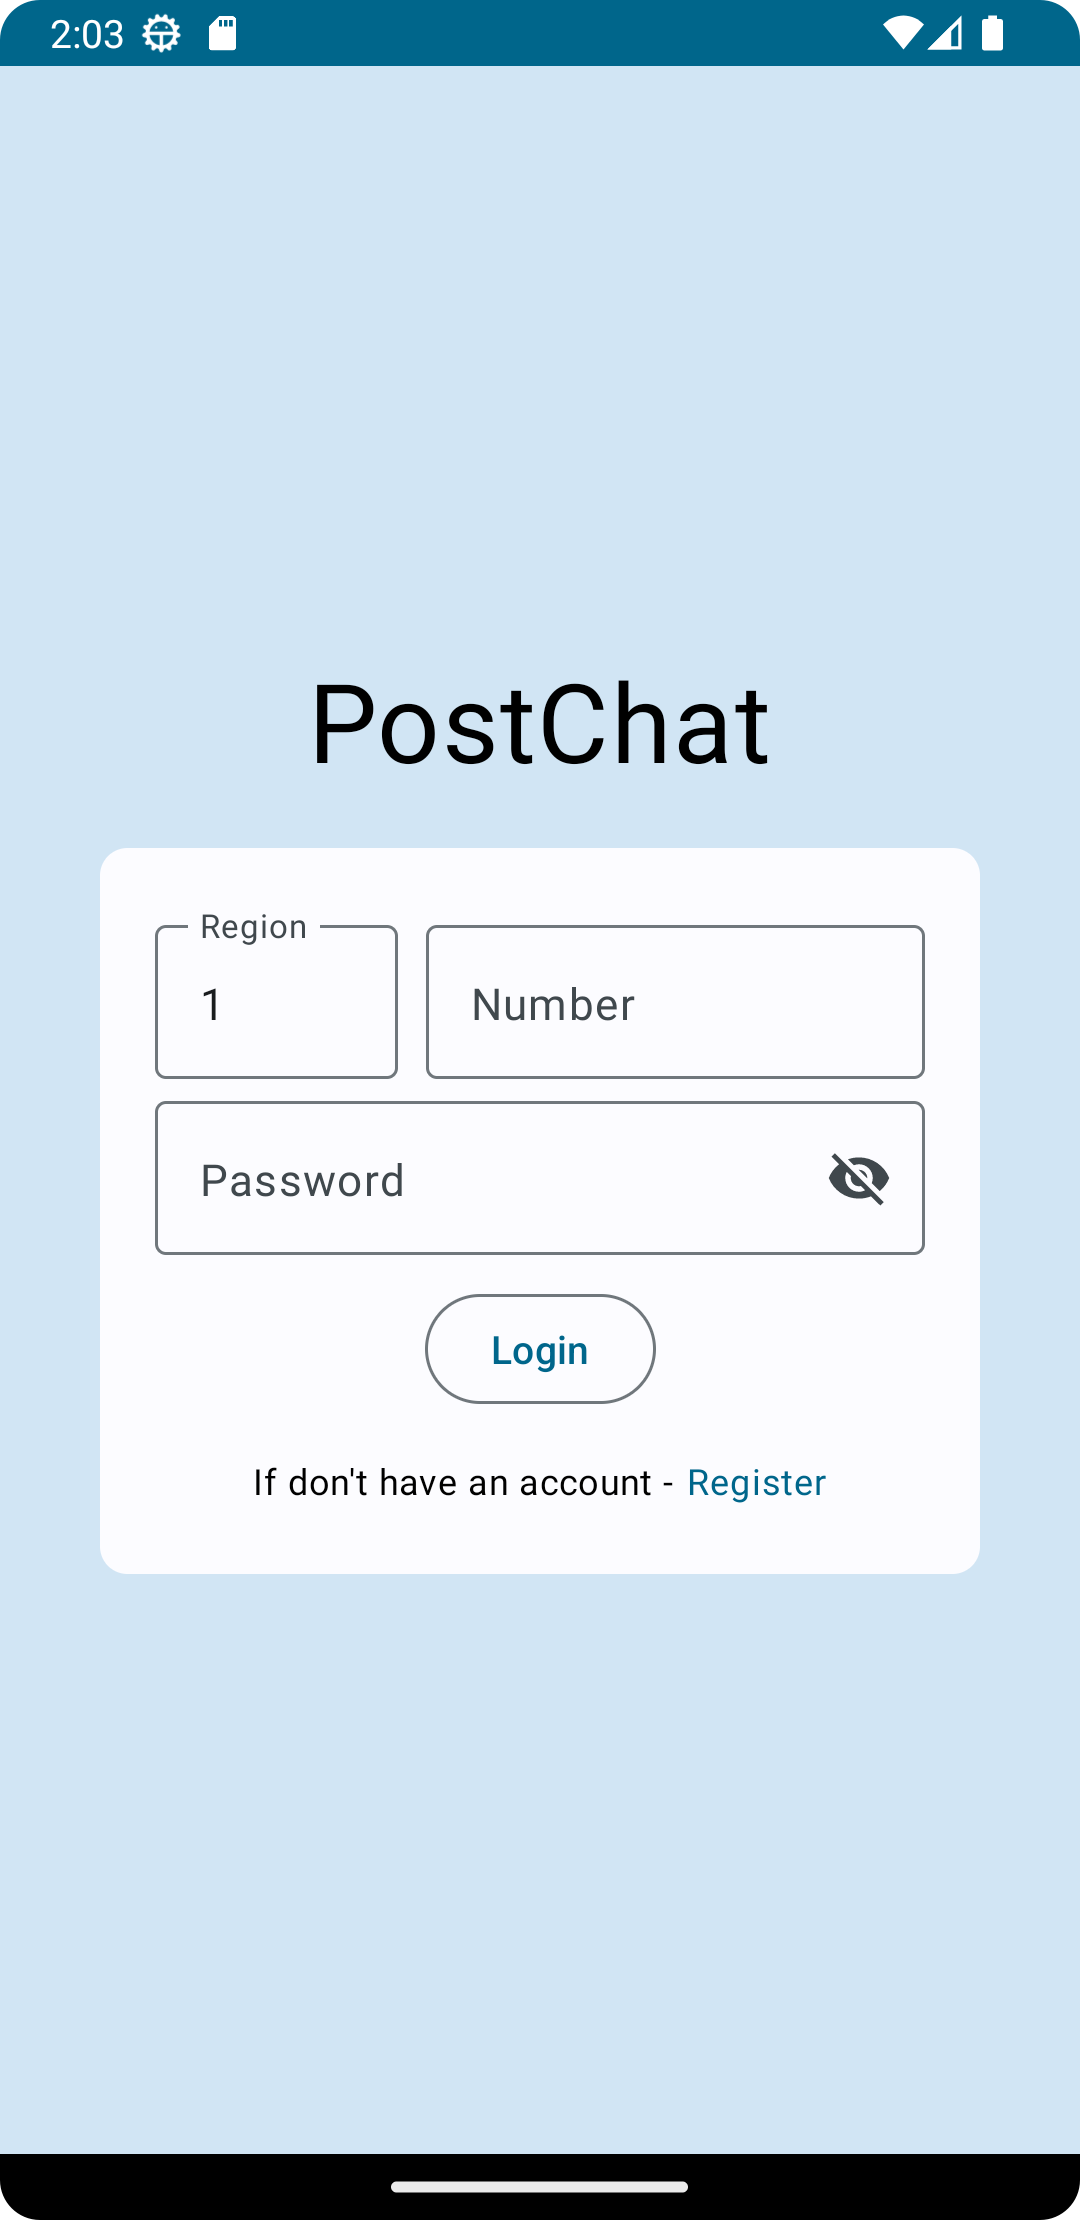
\includegraphics[trim={0cm -3cm 0 -3cm}, width=0.4\textwidth]{./Chapter6/Figures/SignInActivityLogin}
	\caption{Signin Activity}
	\label{fig:SA1}
\end{figure}


It also does local verification's to user's input. Password and Phone Number validations are done using Google's API.

\begin{figure}[!ht]
	\centering
	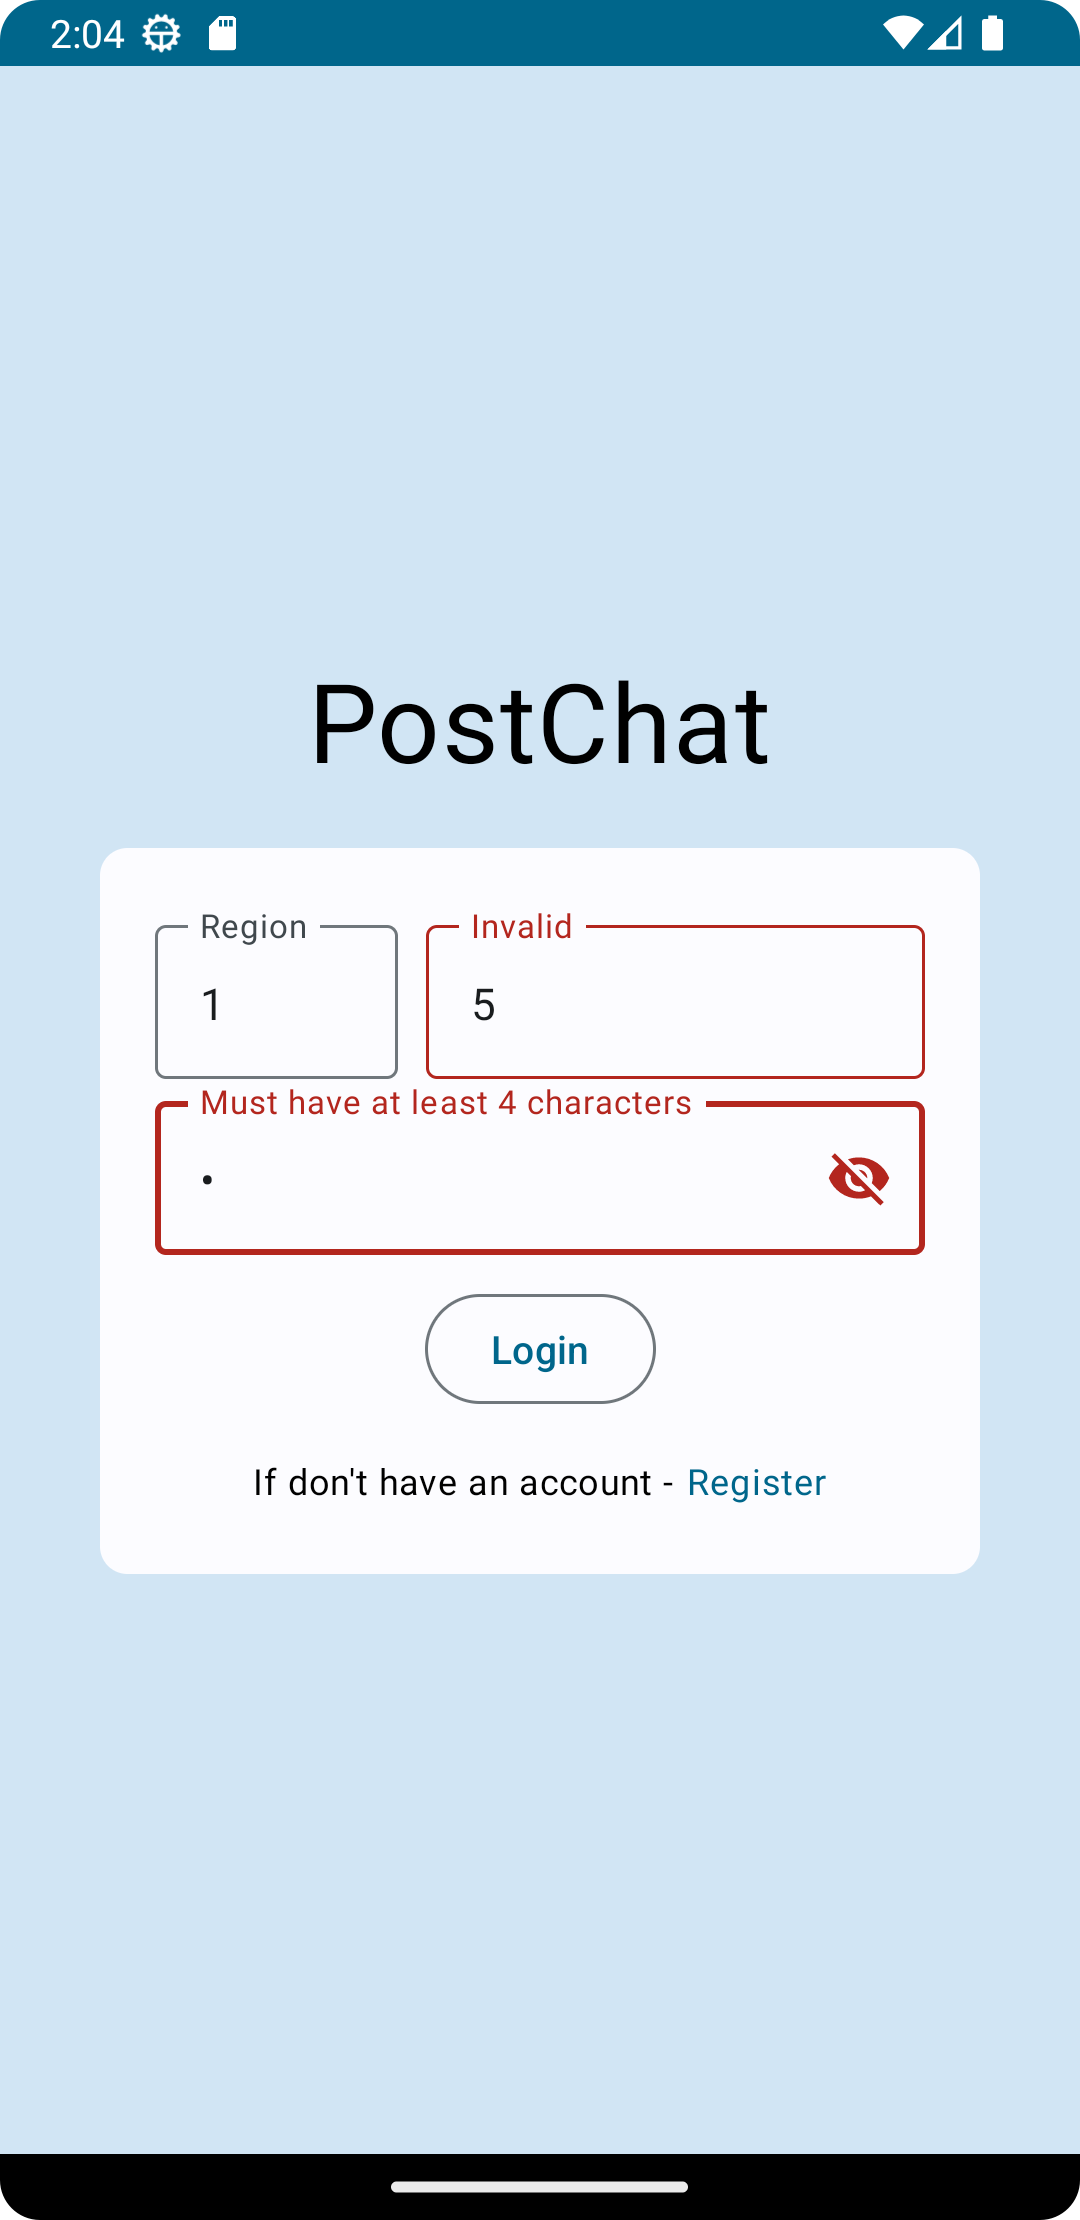
\includegraphics[trim={0cm -3cm 0 -3cm}, width=0.4\textwidth]{./Chapter6/Figures/SignInActivityErrors}
	\caption{Signin Activity invalid password size}
	\label{fig:SA2}
\end{figure}


\subsection{Home}
The Home Activity serves as a central hub for connecting to the web API and retrieving essential information related to registered users, messages, and chats. Its primary purpose is to display all chats in a user-friendly manner, with the chats ordered based on the most recent message received.

By establishing a connection with the web API, the Home Activity can fetch the necessary data to populate the chat interface. It retrieves information about registered users, ensuring that the appropriate user profiles are displayed within the chat list. Additionally, it retrieves messages associated with each chat, allowing users to view their conversation history.

The Home Activity organizes the chats in a manner that prioritizes the most recent interactions. By ordering the chats based on the last message received, users can quickly identify and access their most recent conversations.

Moreover, the Home Activity provides intuitive controls and a simple interface, users can create new chat groups, within a button.

Figure~\ref{fig:HA1} illustrate the implemented activity.

\begin{figure}[!ht]
	\centering
	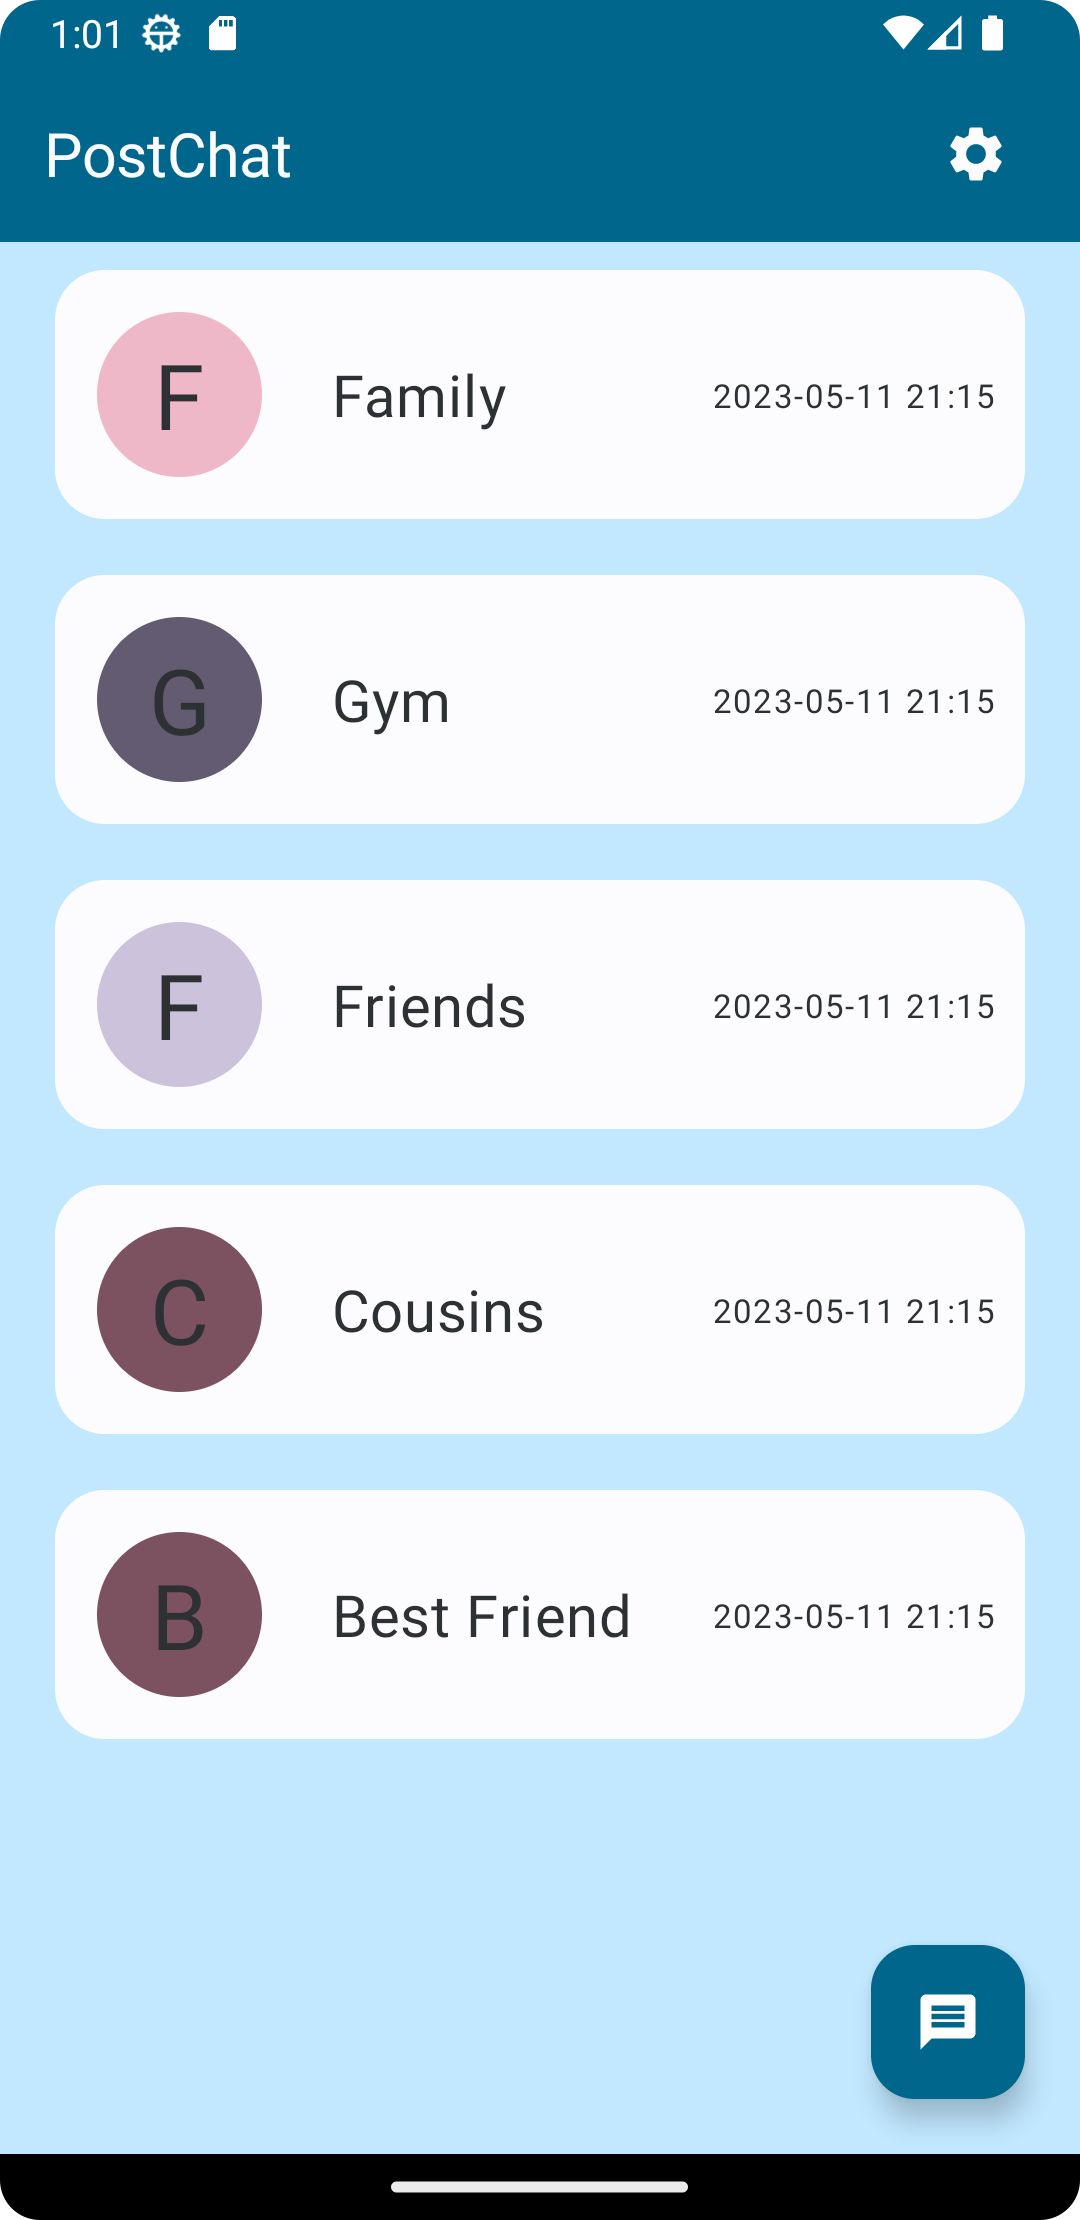
\includegraphics[trim={0cm -3cm 0 -3cm}, width=0.4\textwidth]{./Chapter6/Figures/HomeActivity}
	\caption{Home Activity}
	\label{fig:HA1}
\end{figure}


\subsection{Create Chat}
The CreateChat activity searches for the users stored in the local database and lets you pick the phone numbers you want to add to the chat. Every chat needs a name so a popup dialog input message shows when clicking the check button.

Figures \ref{fig:CCA1} and \ref{fig:CCA2} illustrate the implemented activity.


\begin{figure}[!ht]
	\centering
	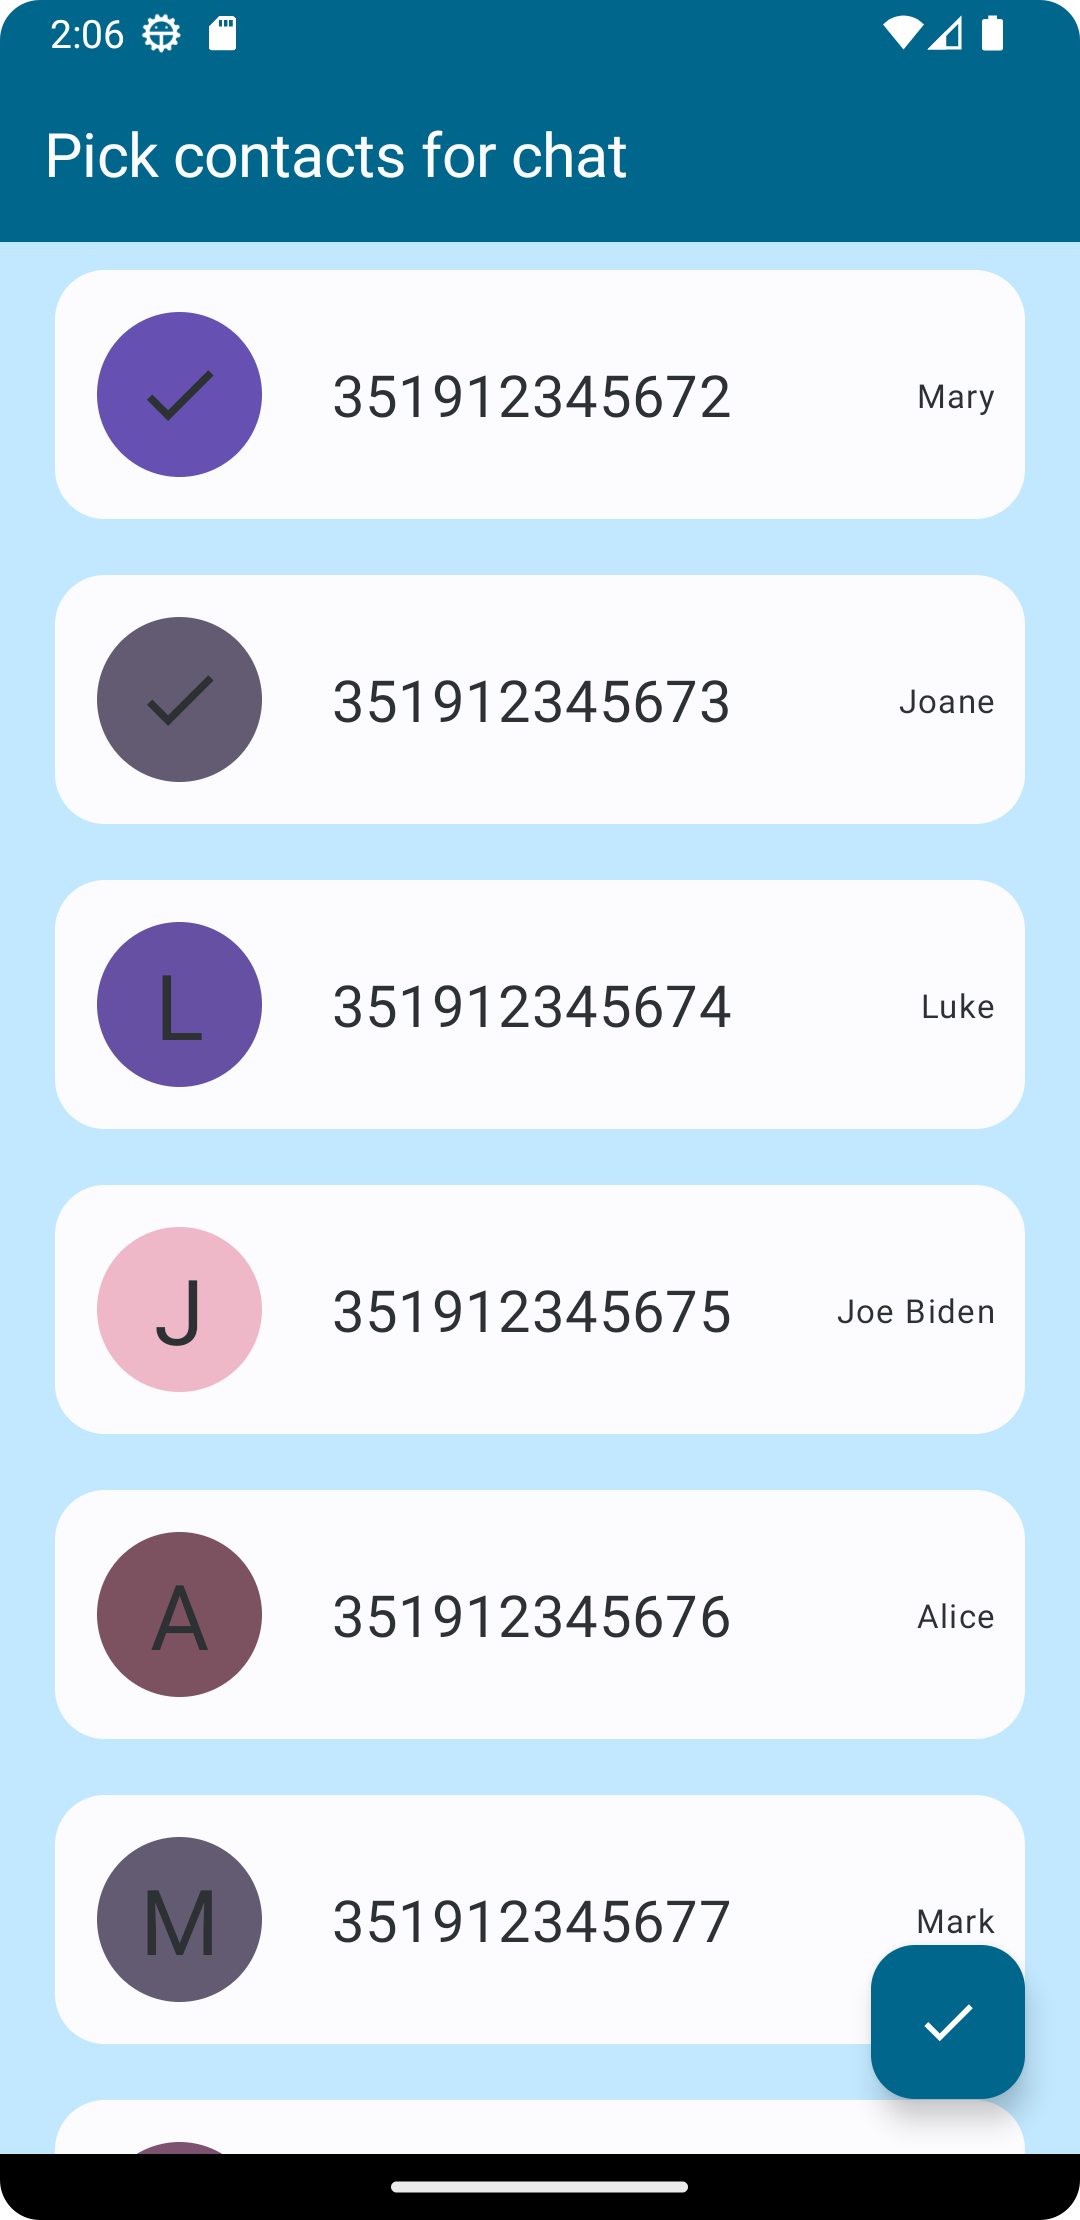
\includegraphics[trim={0cm -3cm 0 -3cm}, width=0.4\textwidth]{./Chapter6/Figures/CreateChatActivityPickContacts}
	\caption{CreateChat Activity}
	\label{fig:CCA1}
\end{figure}


\begin{figure}[!ht]
	\centering
	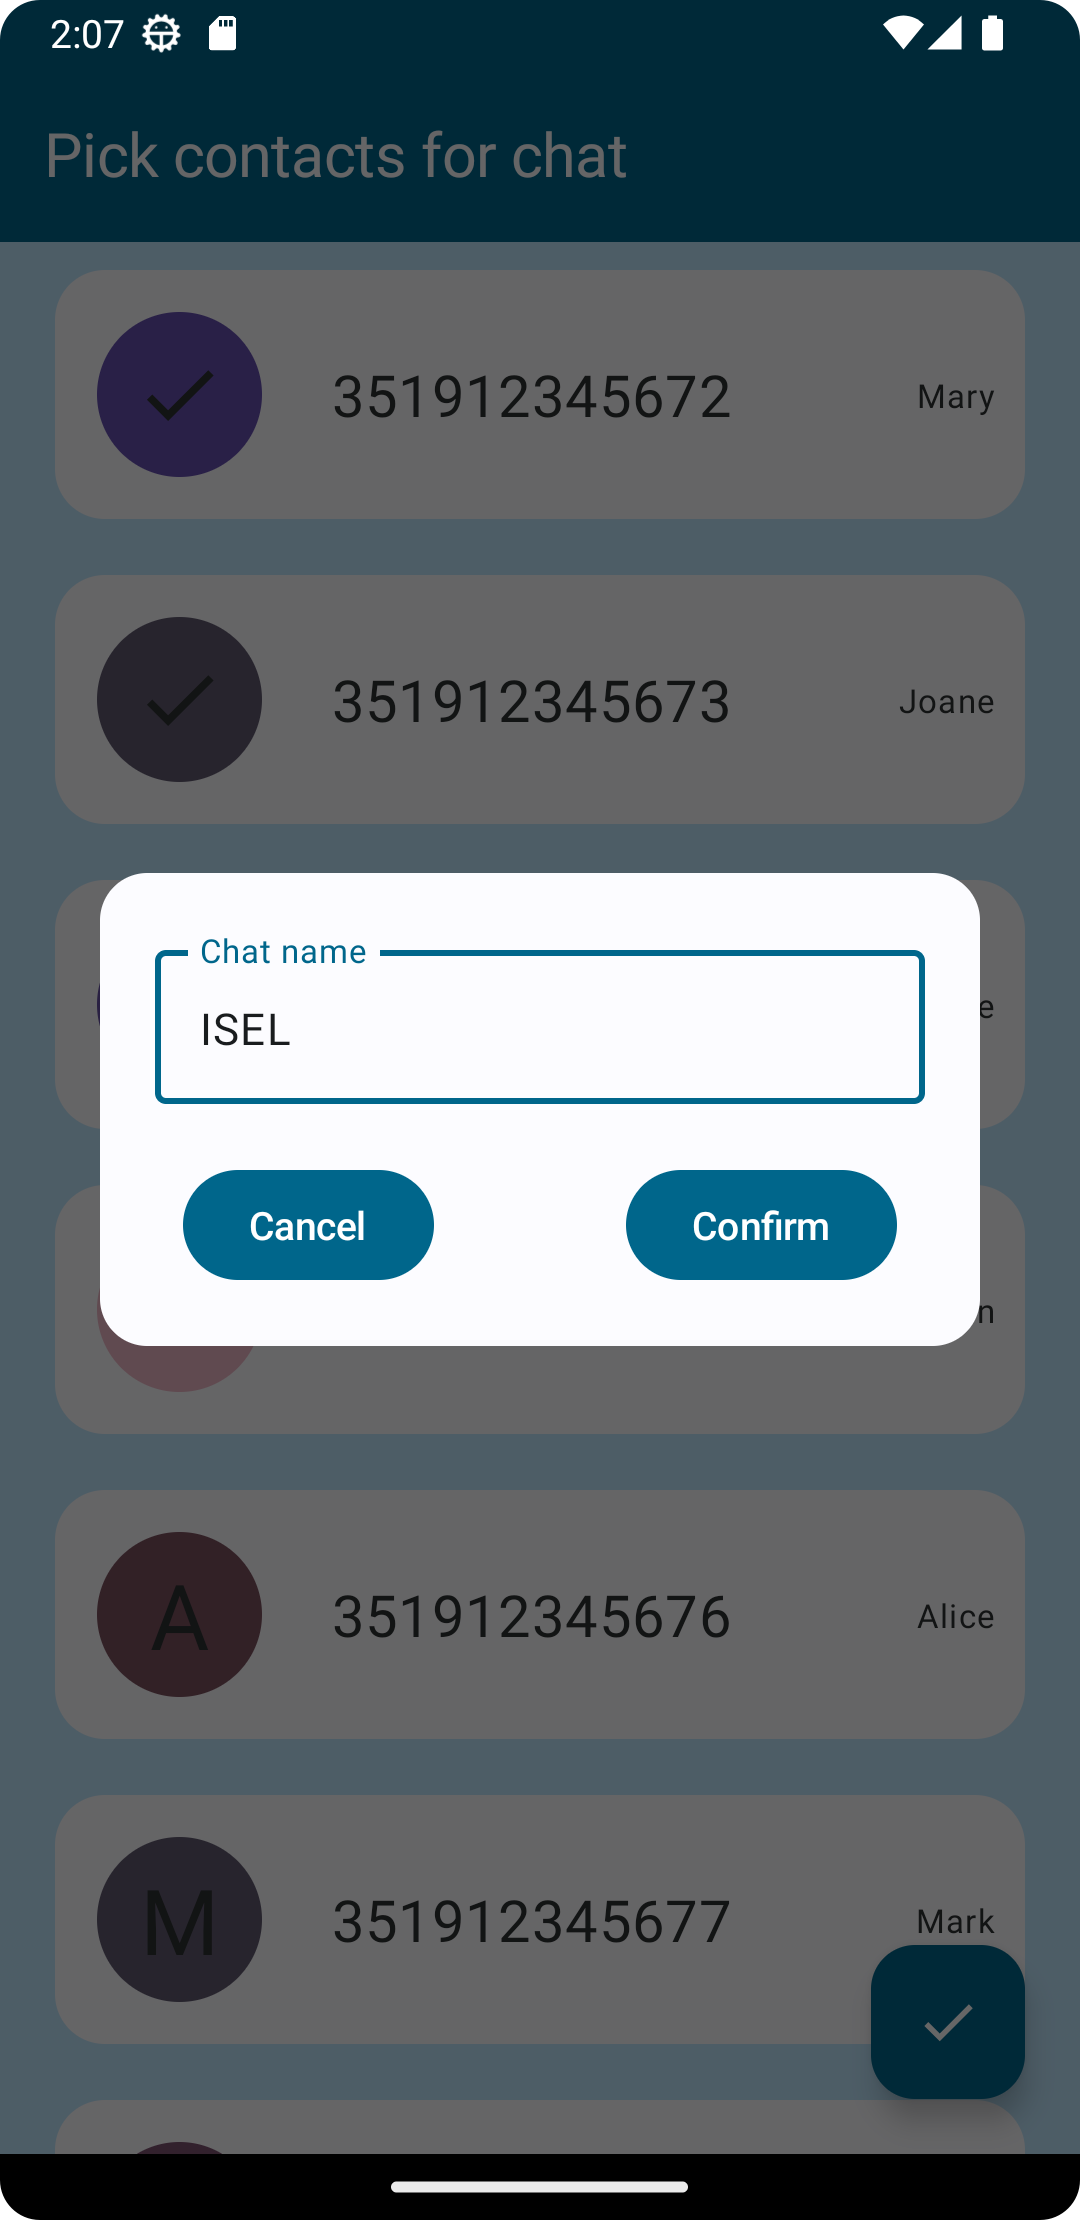
\includegraphics[trim={0cm -3cm 0 -3cm}, width=0.4\textwidth]{./Chapter6/Figures/CreateChatActivityName}
	\caption{CreateChat Activity name prompt}
	\label{fig:CCA2}
\end{figure}

\subsection{Chat View}
The Chat activity obtains the information about the current chat messages. 
It displays the postcards in order by the timestamp and above the same it shows the number from the person that sent the message. In the future this will be changed to query users in the local database and get their name.  

Figures \ref{fig:CVA1}, \ref{fig:CVA2} , \ref{fig:CVA3} and \ref{fig:CVA4} illustrate the implemented activity.

\begin{figure}[!ht]
	\centering
	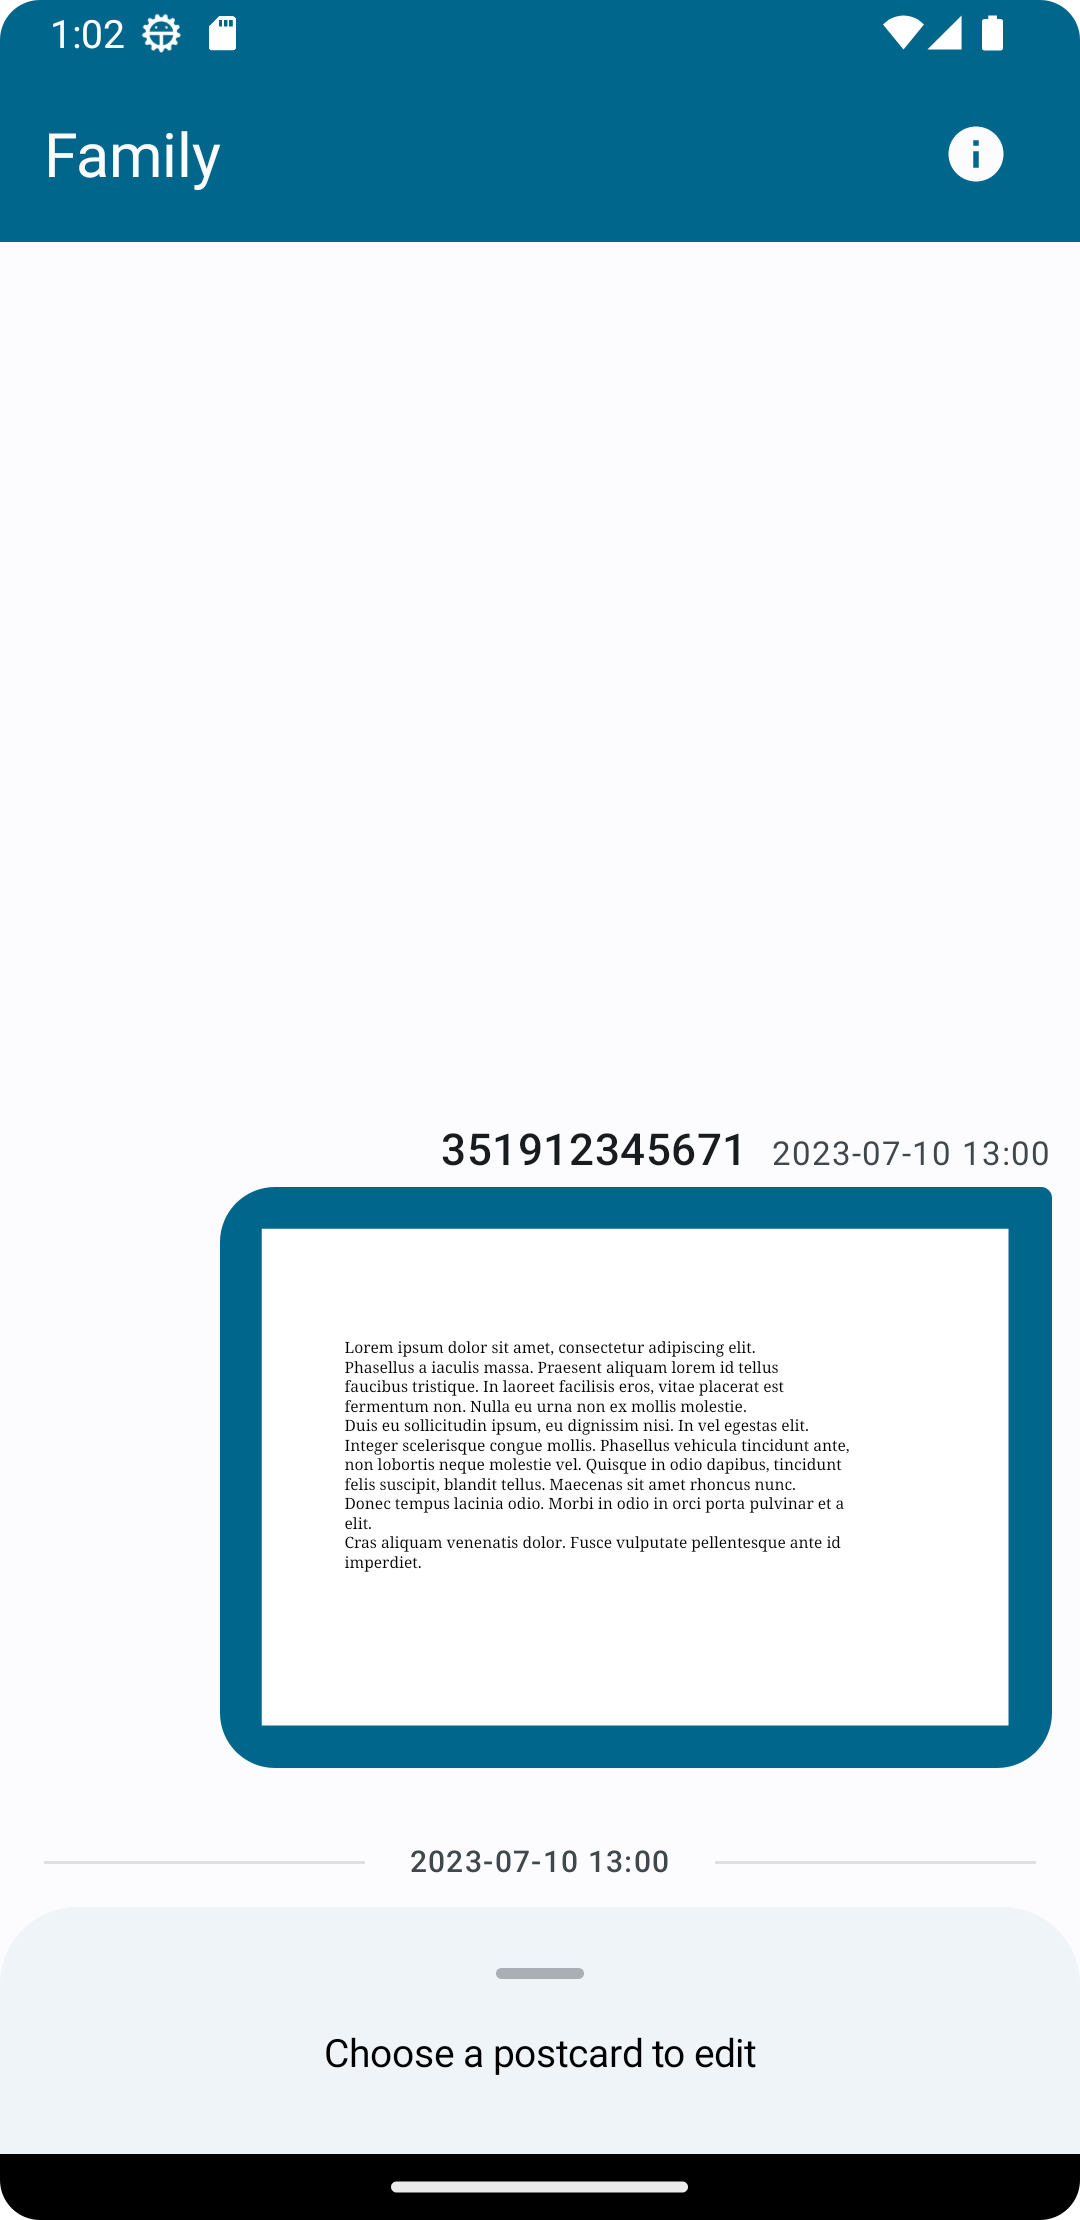
\includegraphics[trim={0cm -3cm 0 -3cm}, width=0.4\textwidth]{./Chapter6/Figures/ChatActivity}
	\caption{Chat Activity}
	\label{fig:CVA1}
\end{figure}


\begin{figure}[!ht]
	\centering
	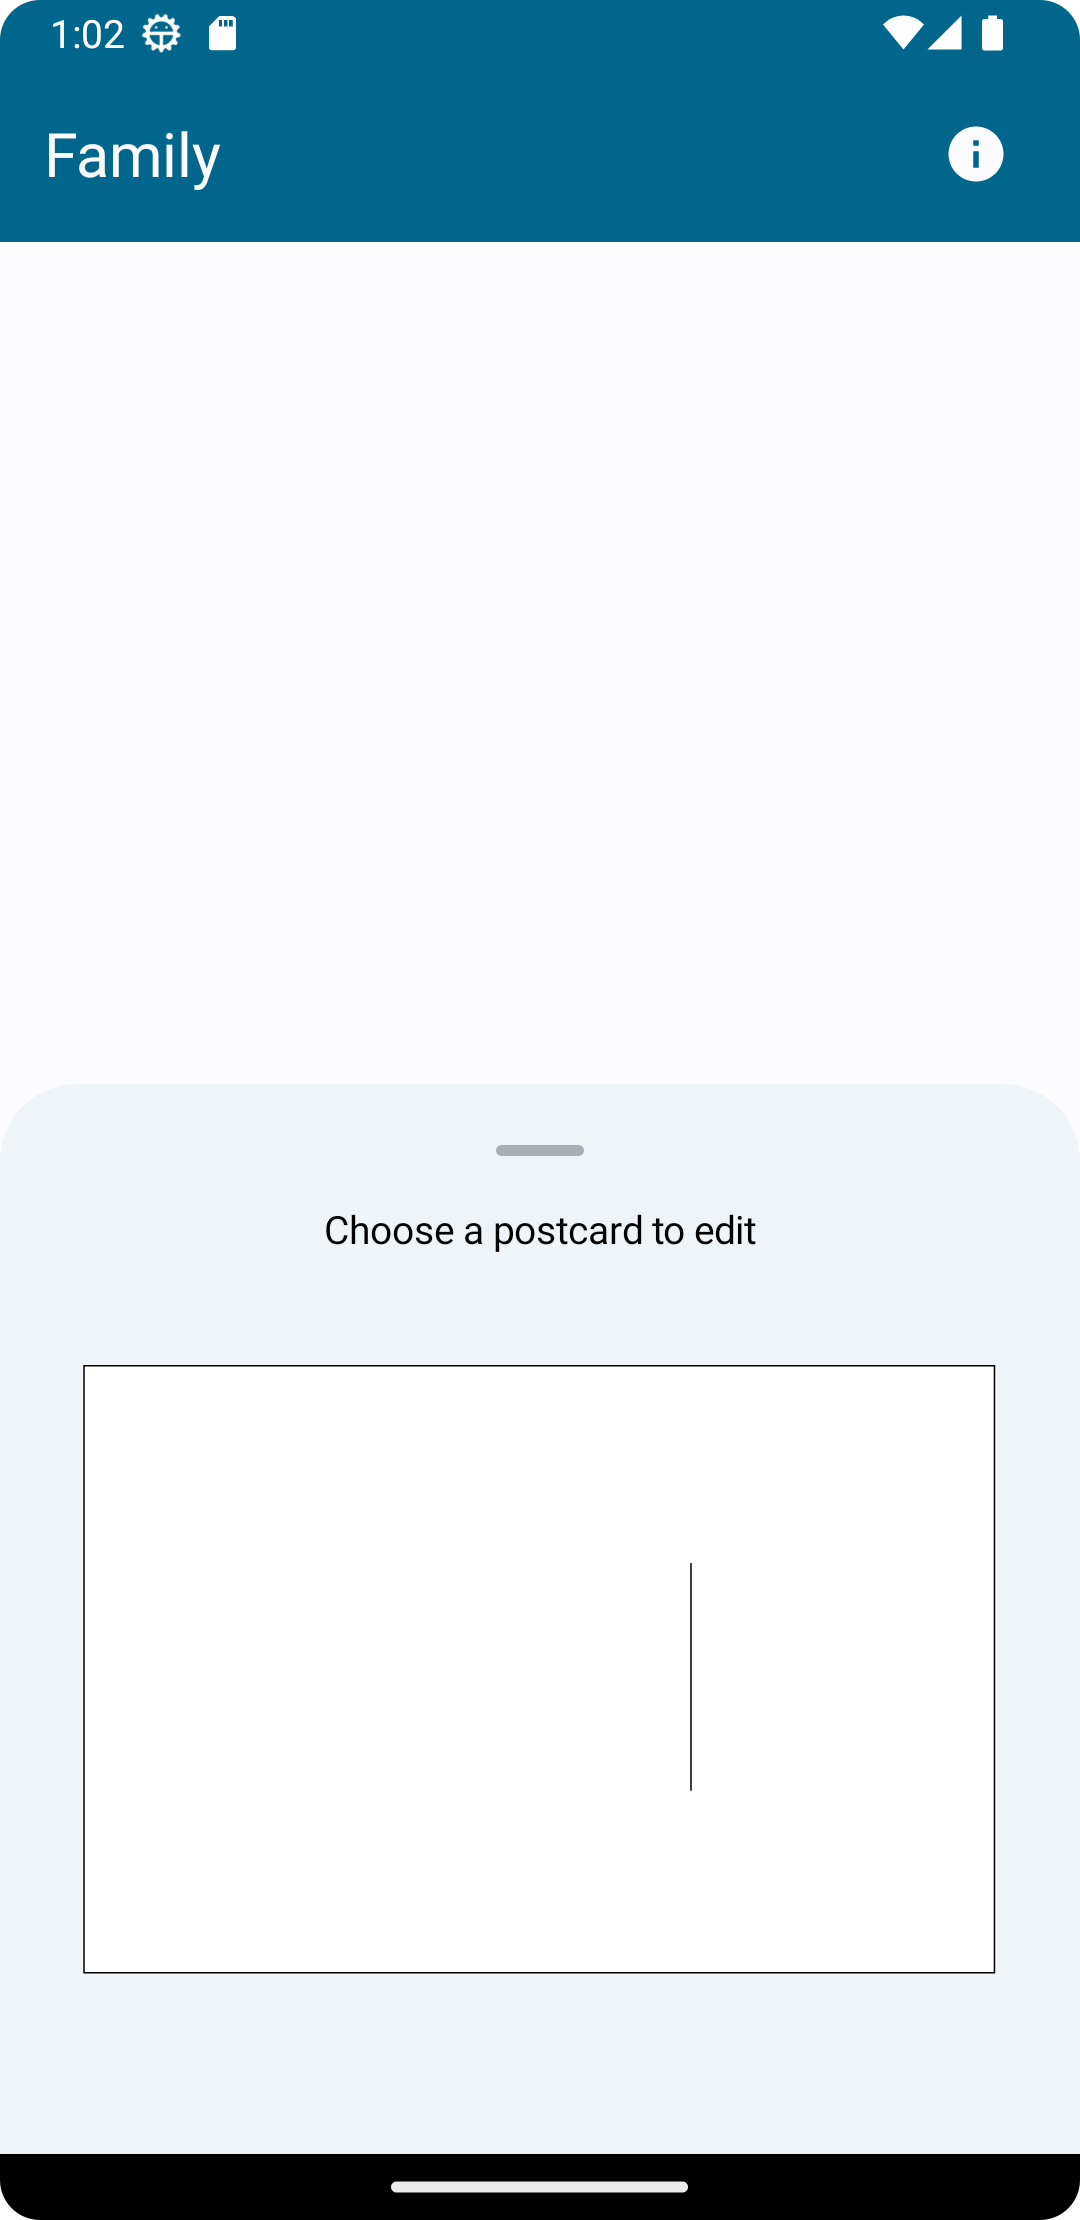
\includegraphics[trim={0cm -3cm 0 -3cm}, width=0.4\textwidth]{./Chapter6/Figures/ChatActivityShowPostcards}
	\caption{Chat Activity bottom templates list}
	\label{fig:CVA2}
\end{figure}


\begin{figure}[!ht]
	\centering
	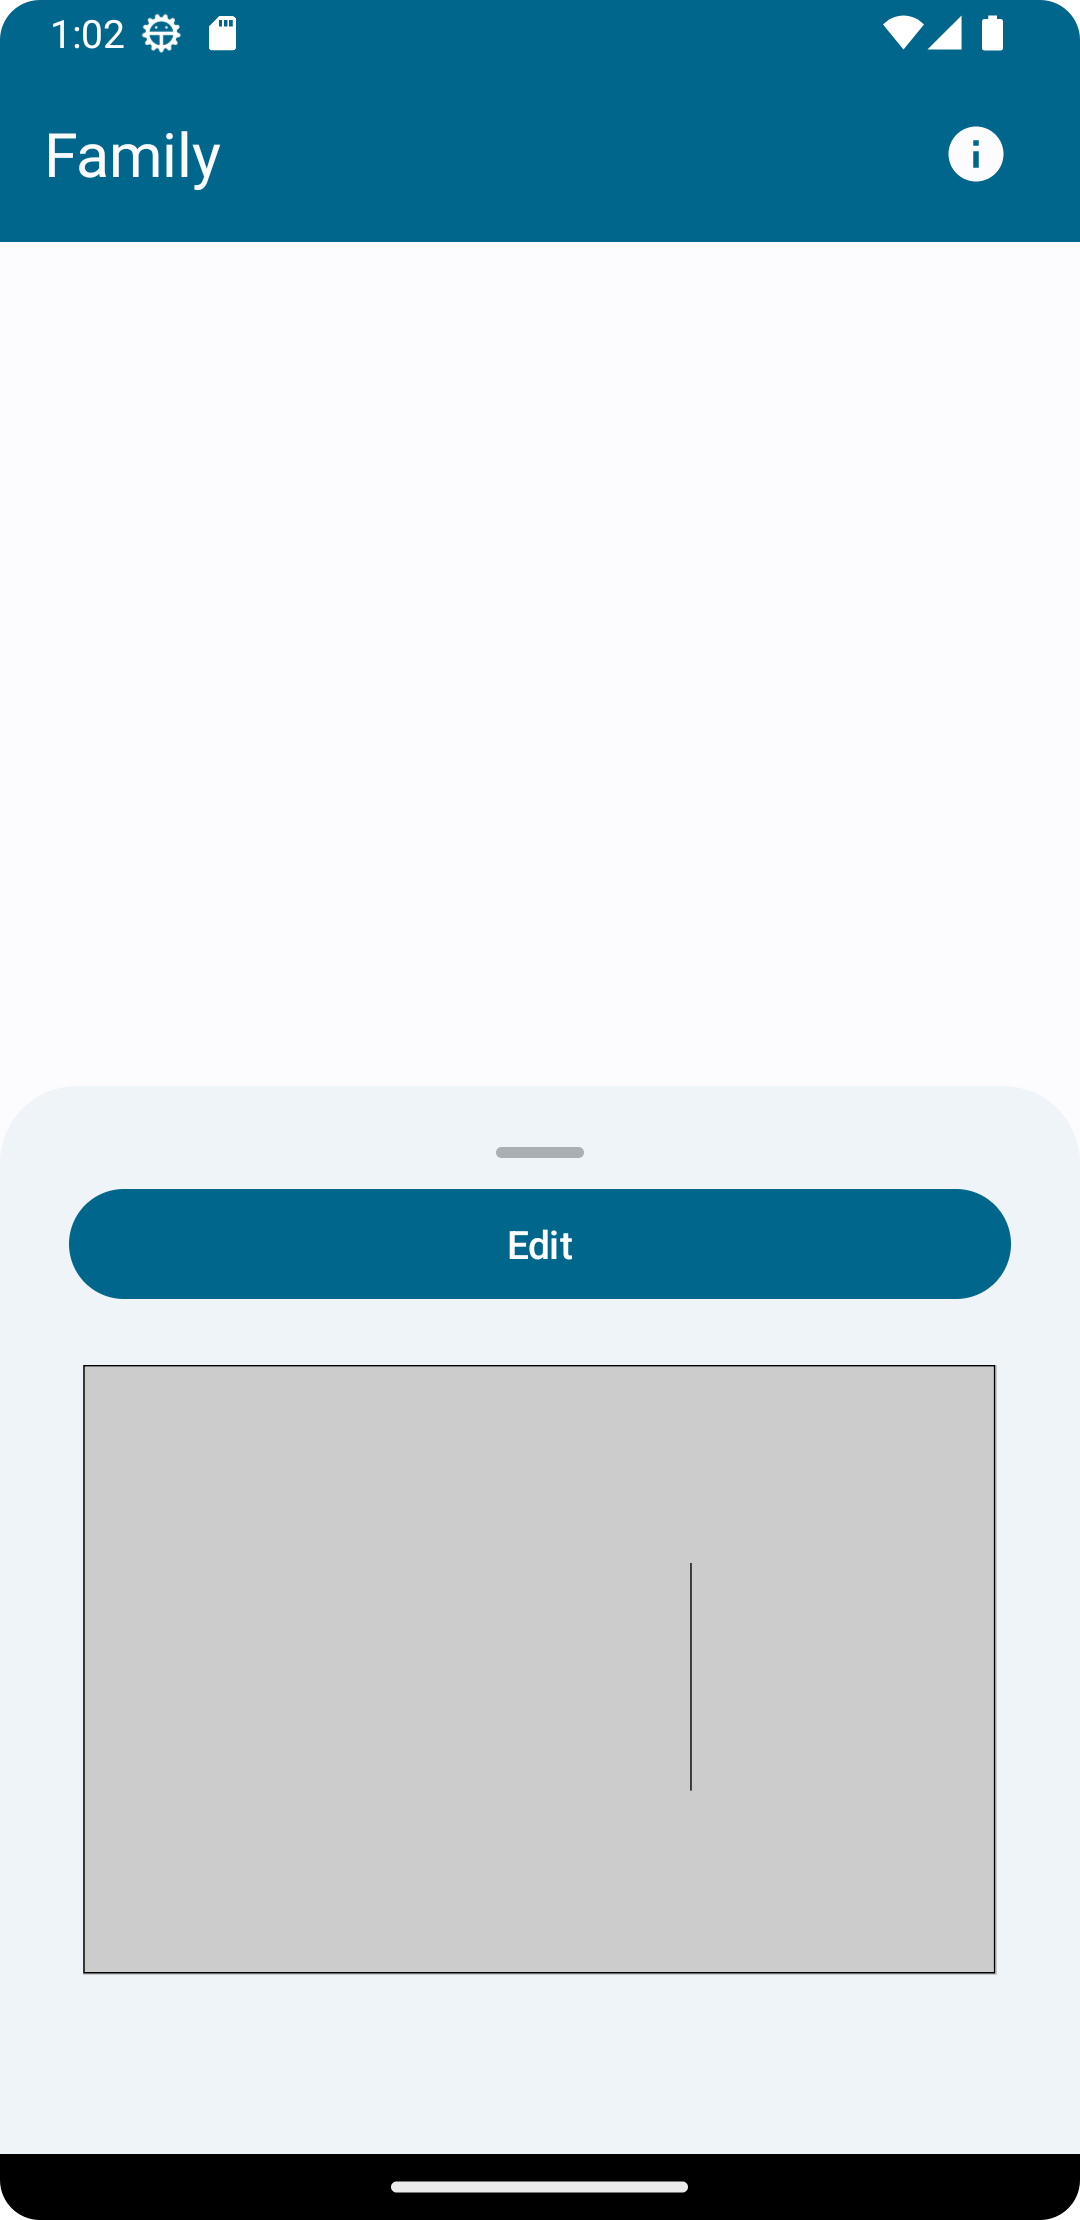
\includegraphics[trim={0cm -3cm 0 -3cm}, width=0.4\textwidth]{./Chapter6/Figures/ChatActivityPickPostcard}
	\caption{Chat Activity pick template}
	\label{fig:CVA3}
\end{figure}

On clicking the edit button the user is sent to the Draw Activity.

\begin{figure}[!ht]
	\centering
	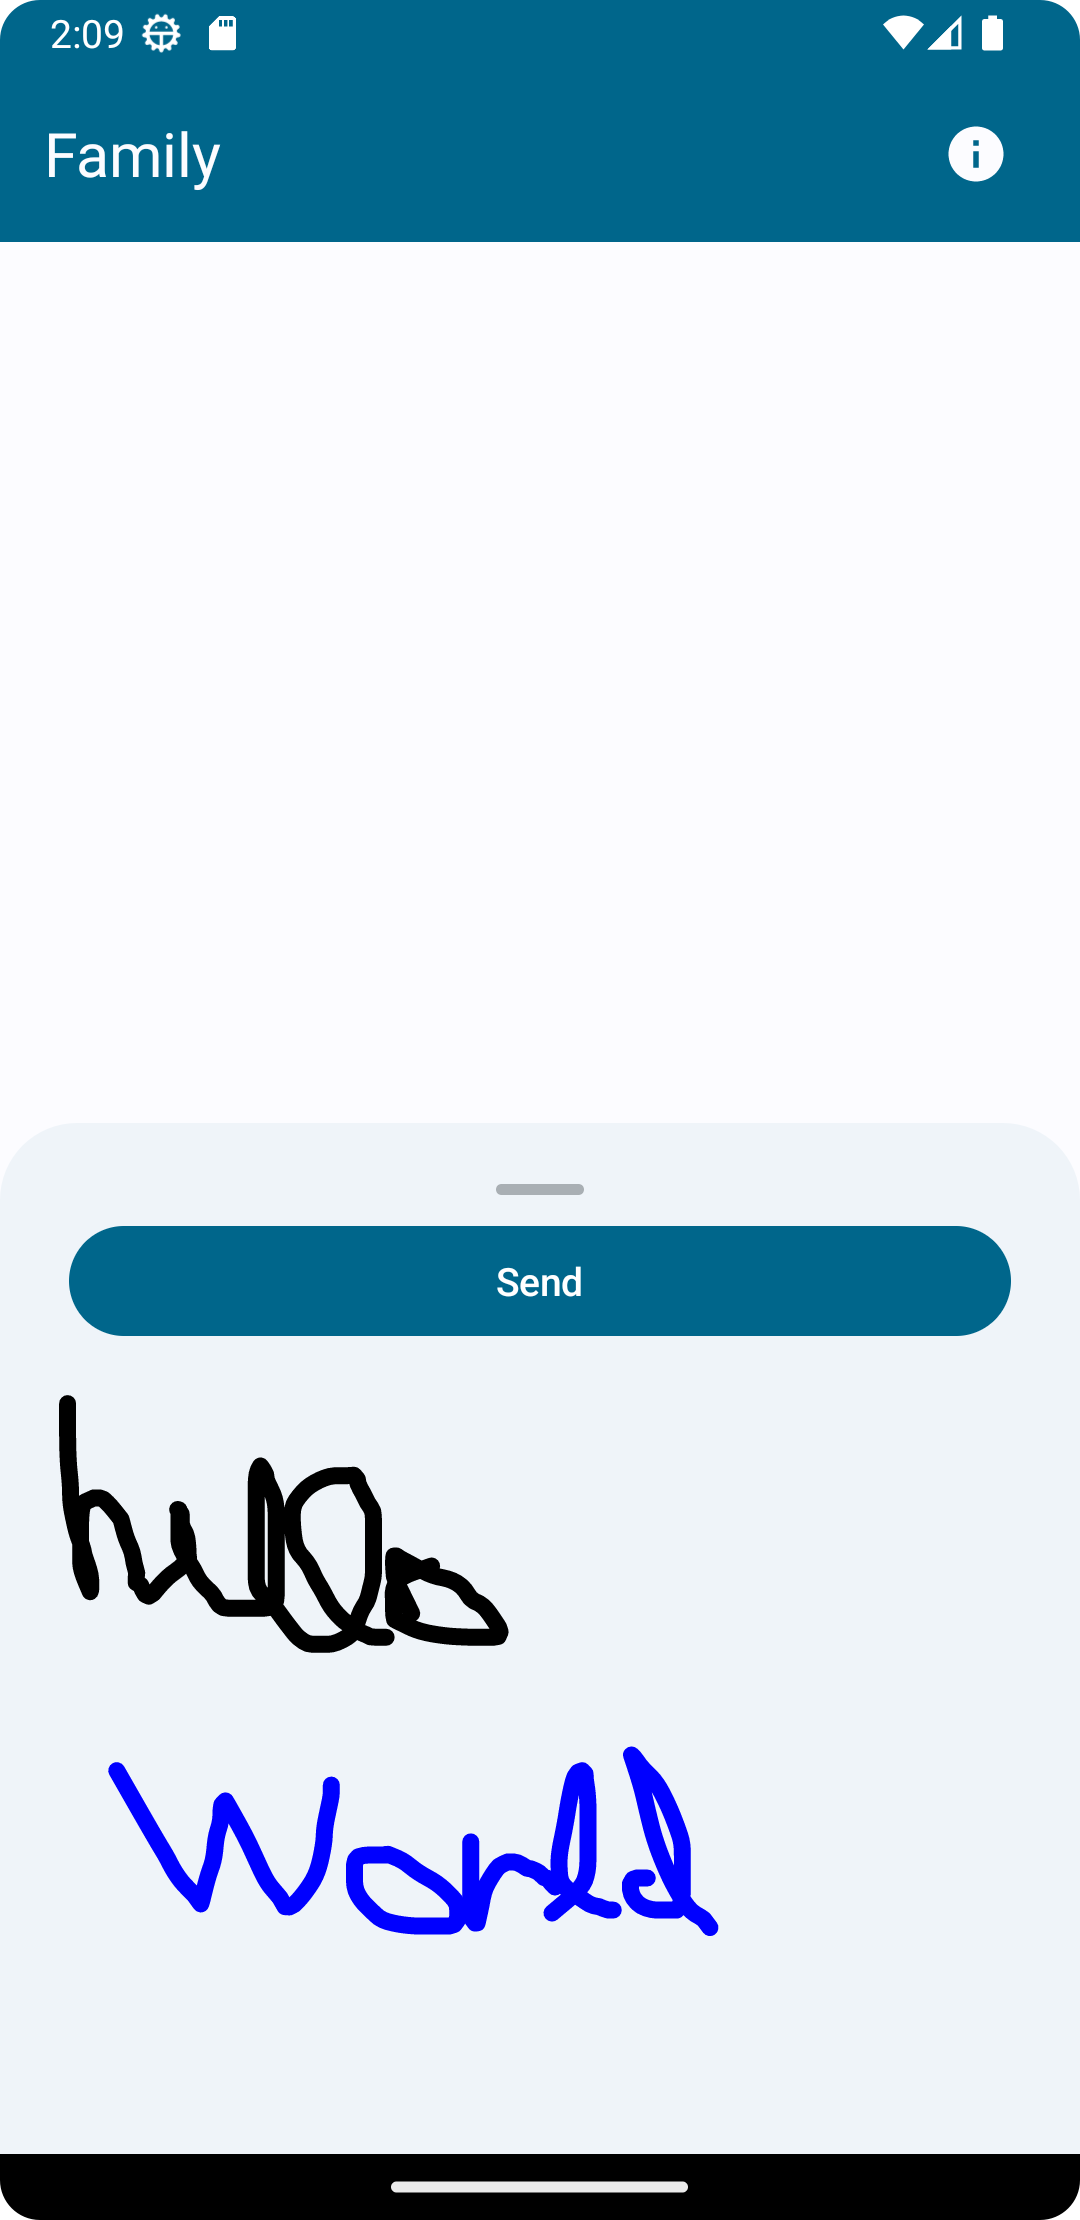
\includegraphics[trim={0cm -3cm 0 -3cm}, width=0.4\textwidth]{./Chapter6/Figures/ChatActivityPreview}
	\caption{CreateChat preview postcard}
	\label{fig:CVA4}
\end{figure}


\begin{figure}[!ht]
	\centering
	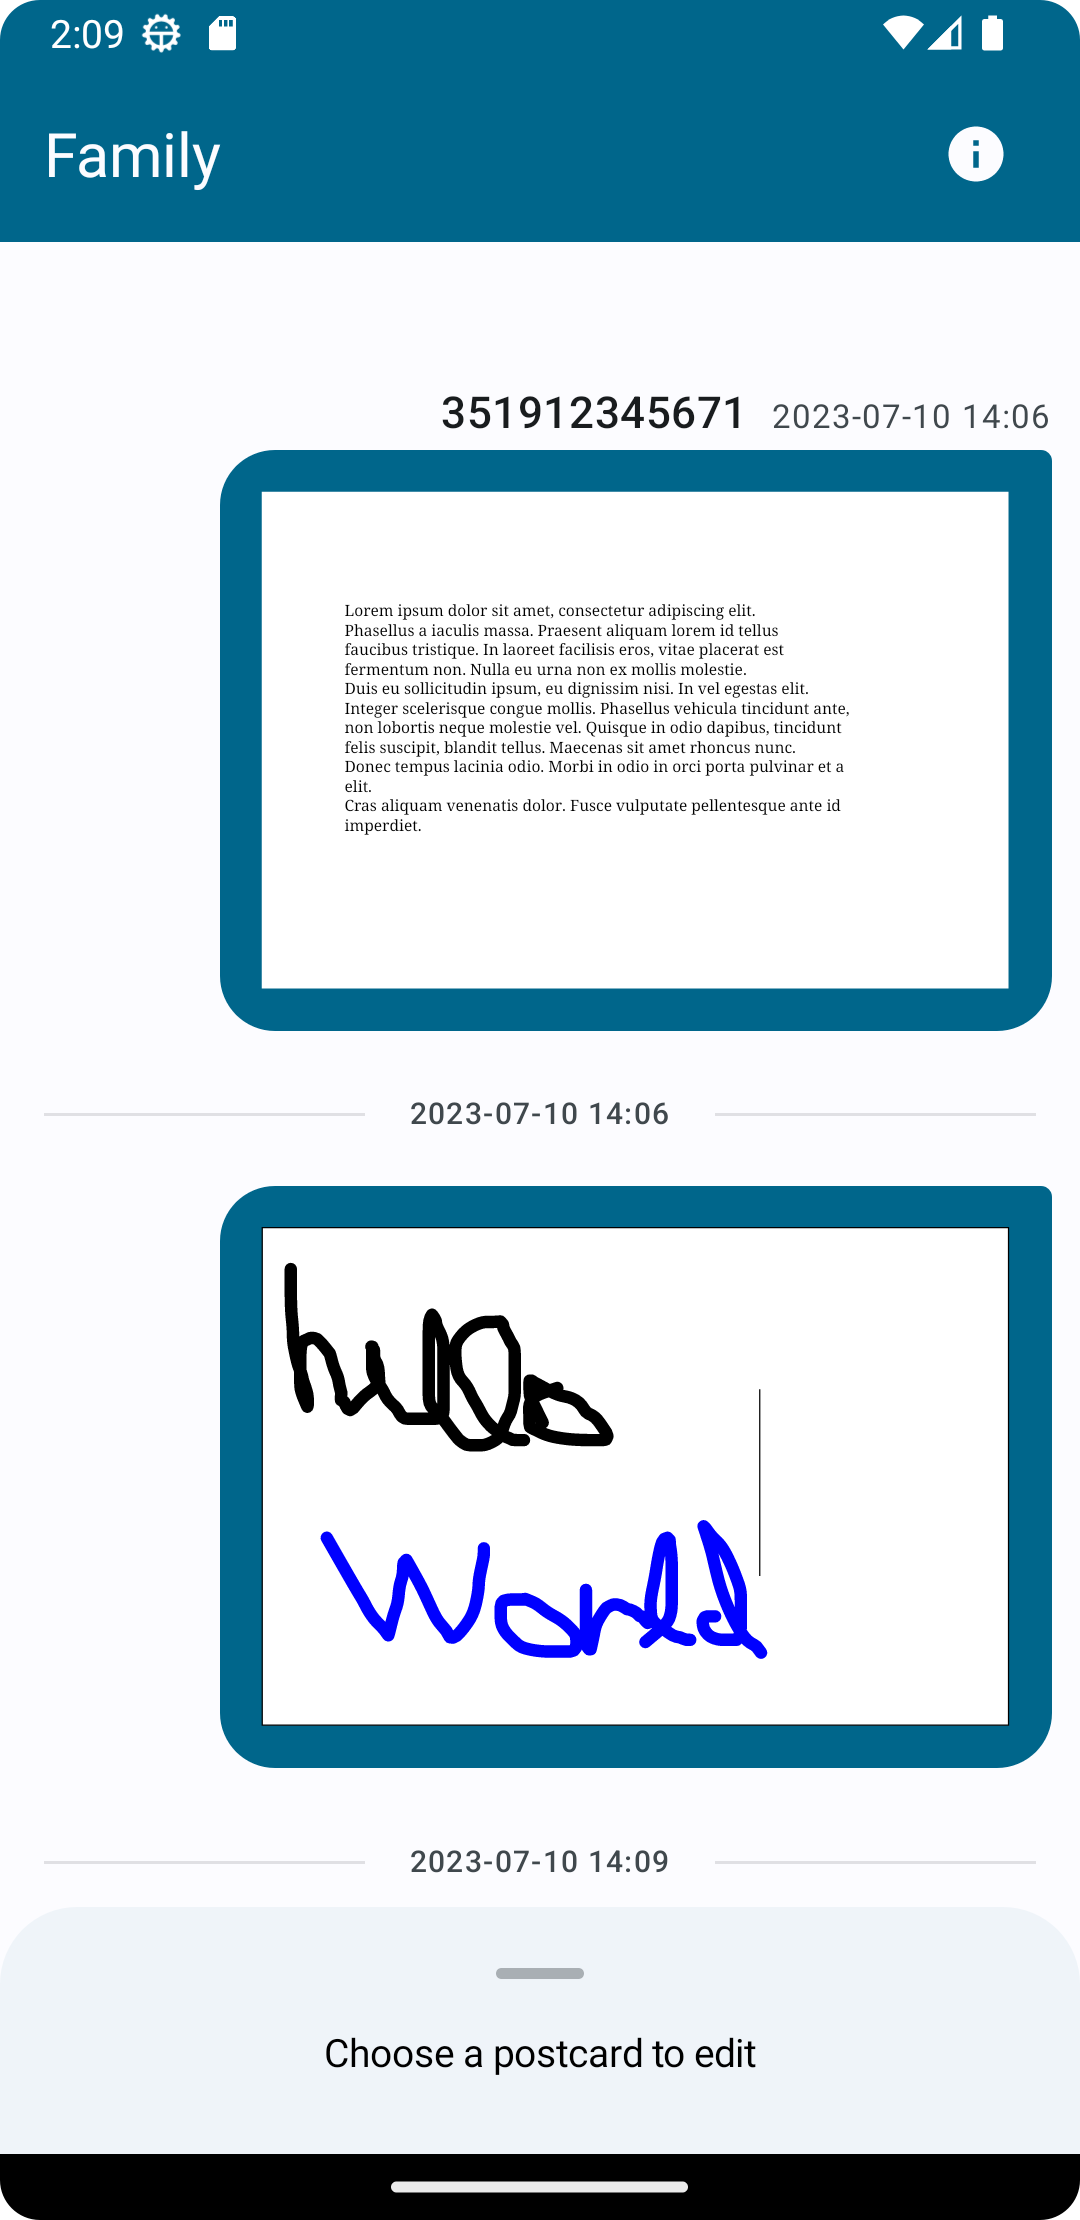
\includegraphics[trim={0cm -3cm 0 -3cm}, width=0.4\textwidth]{./Chapter6/Figures/ChatActivityUpdated}
	\caption{CreateChat postcard sent}
	\label{fig:CVA4}
\end{figure}



\subsection{Draw Postcard}
The Draw activity plays a crucial role in allowing users to edit and personalize a postcard using the Canvas. It involves implementing complex code to enable features such as drawing, zooming, and saving the postcard.

The challenge in implementing drawing and zoom features arise from the absence of a built-in two-finger zoom and one-finger touch draw function in the compose toolkit. To overcome this limitation, an in-depth analysis of the compose toolkit's inner code was conducted. By examining the underlying mechanisms of the compose toolkit, the necessary functionality for drawing and zooming was achieved.

To facilitate the saving of the canvas, a list is used to store the properties of each path. Each path property consists of the actual path data and the stroke style applied to it. When the canvas needs to be saved, the application iterates through each path in the list and generates an SVG file.

During the SVG file creation process, the application adds the necessary path movements and stroke styles to accurately represent each drawn path. This ensures that the saved SVG file faithfully represents the visual appearance of the canvas.

Figures \ref{fig:DA1} illustrate the implemented activity.



\begin{figure}[!ht]
	\centering
	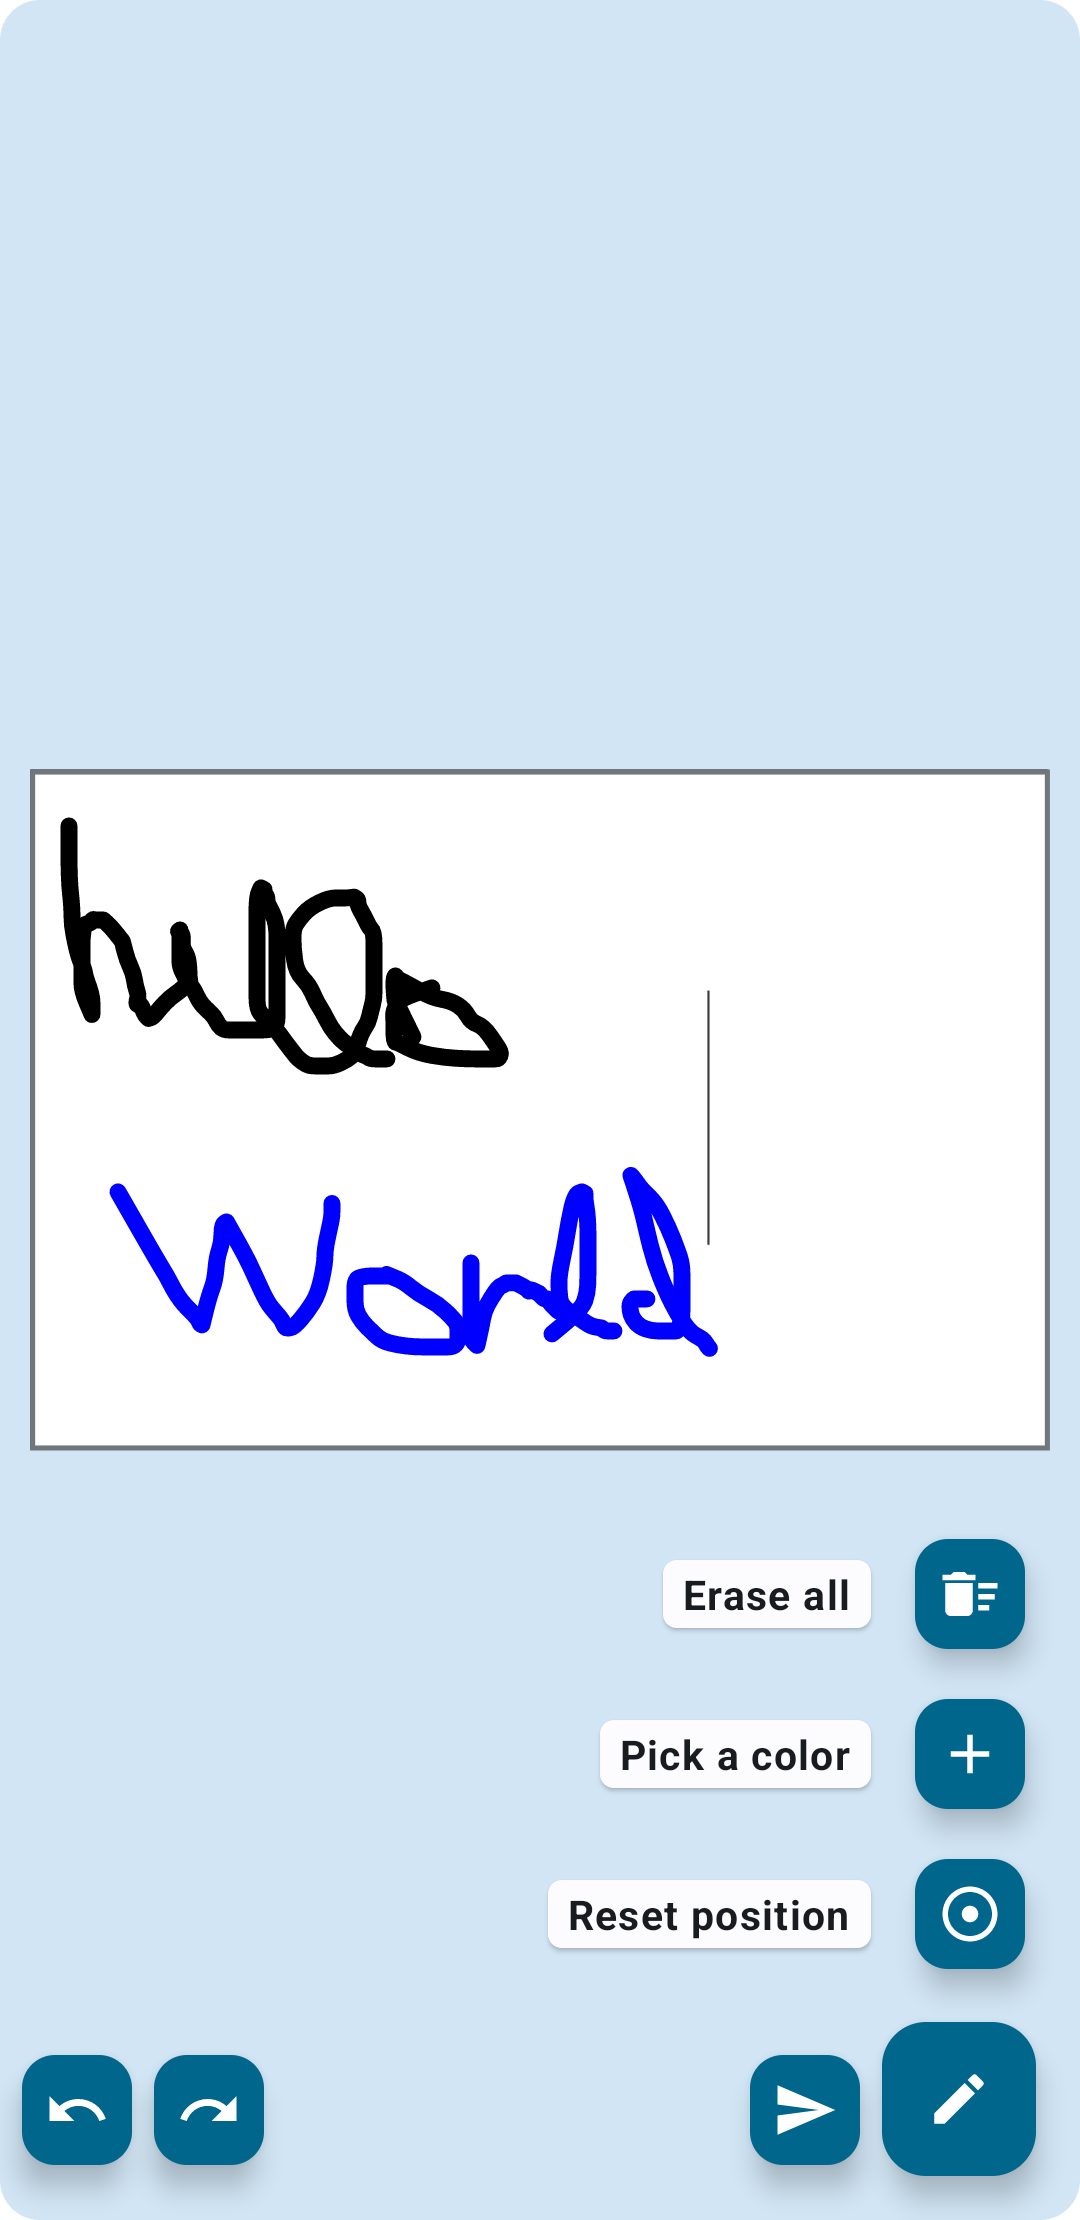
\includegraphics[trim={0cm -3cm 0 -3cm}, width=0.4\textwidth]{./Chapter6/Figures/DrawActivity}
	\caption{Draw Activity}
	\label{fig:DA1}
\end{figure}


\subsection{View Postcard}
The View Postcard Activity provides users with a dedicated interface to view postcards. It offers the ability to save and perform HTR over a postcard. 
When saving a file the user is prompted to choose the quality (from 1 to 5) this will multiply the default width and height of the SVG by the chosen value. The postcard is saved in the images media folder.
This activity focuses on delivering a seamless and immersive experience for users to enjoy the postcard content.

Figures \ref{fig:VA}, \ref{fig:VA1} and \ref{fig:VA2} illustrate the implemented activity.

\begin{figure}[!ht]
	\centering
	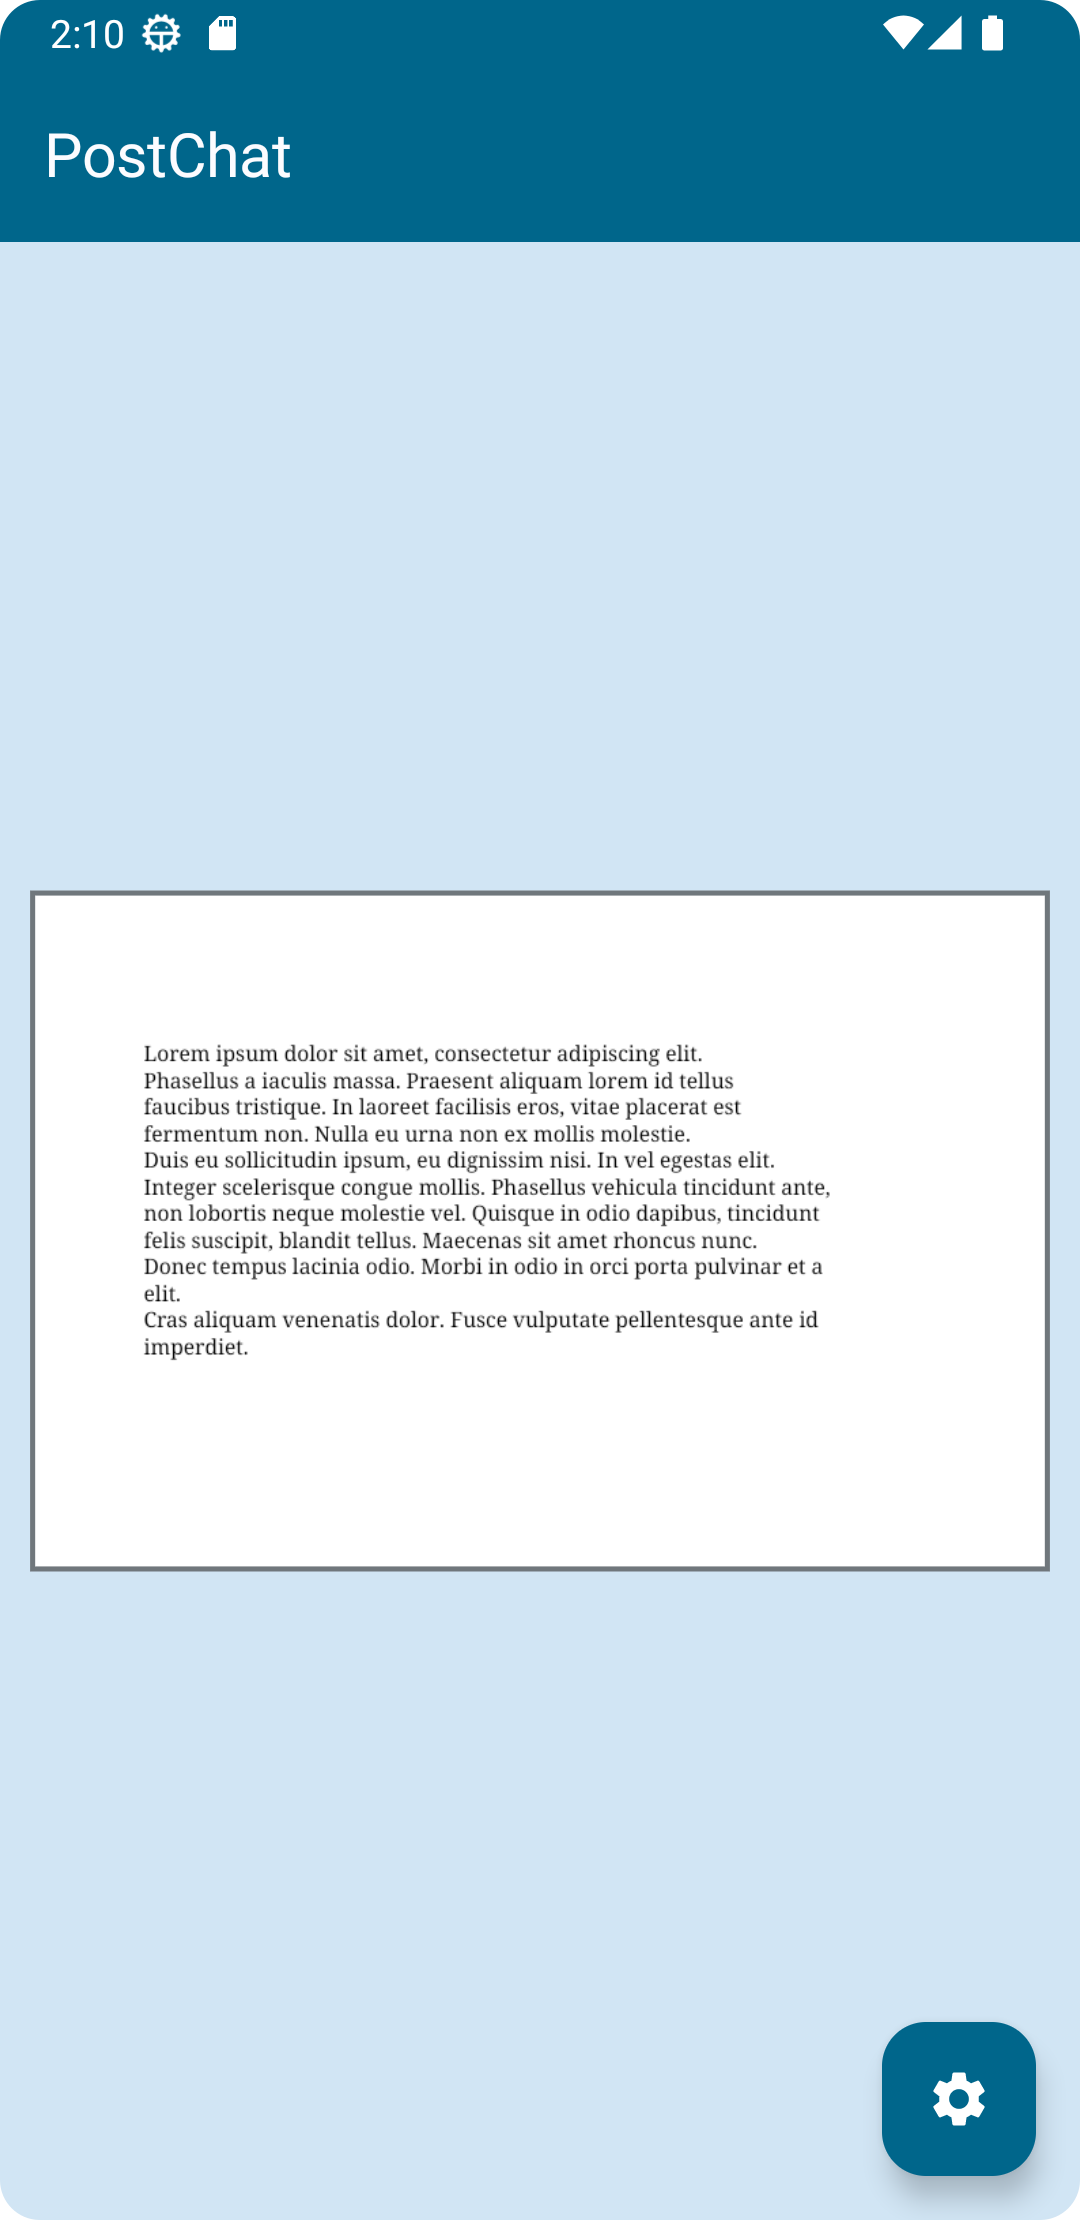
\includegraphics[trim={0cm -3cm 0 -3cm}, width=0.4\textwidth]{./Chapter6/Figures/PostcardActivity}
	\caption{Postcard View}
	\label{fig:VA}
\end{figure}


\begin{figure}[!ht]
	\centering
	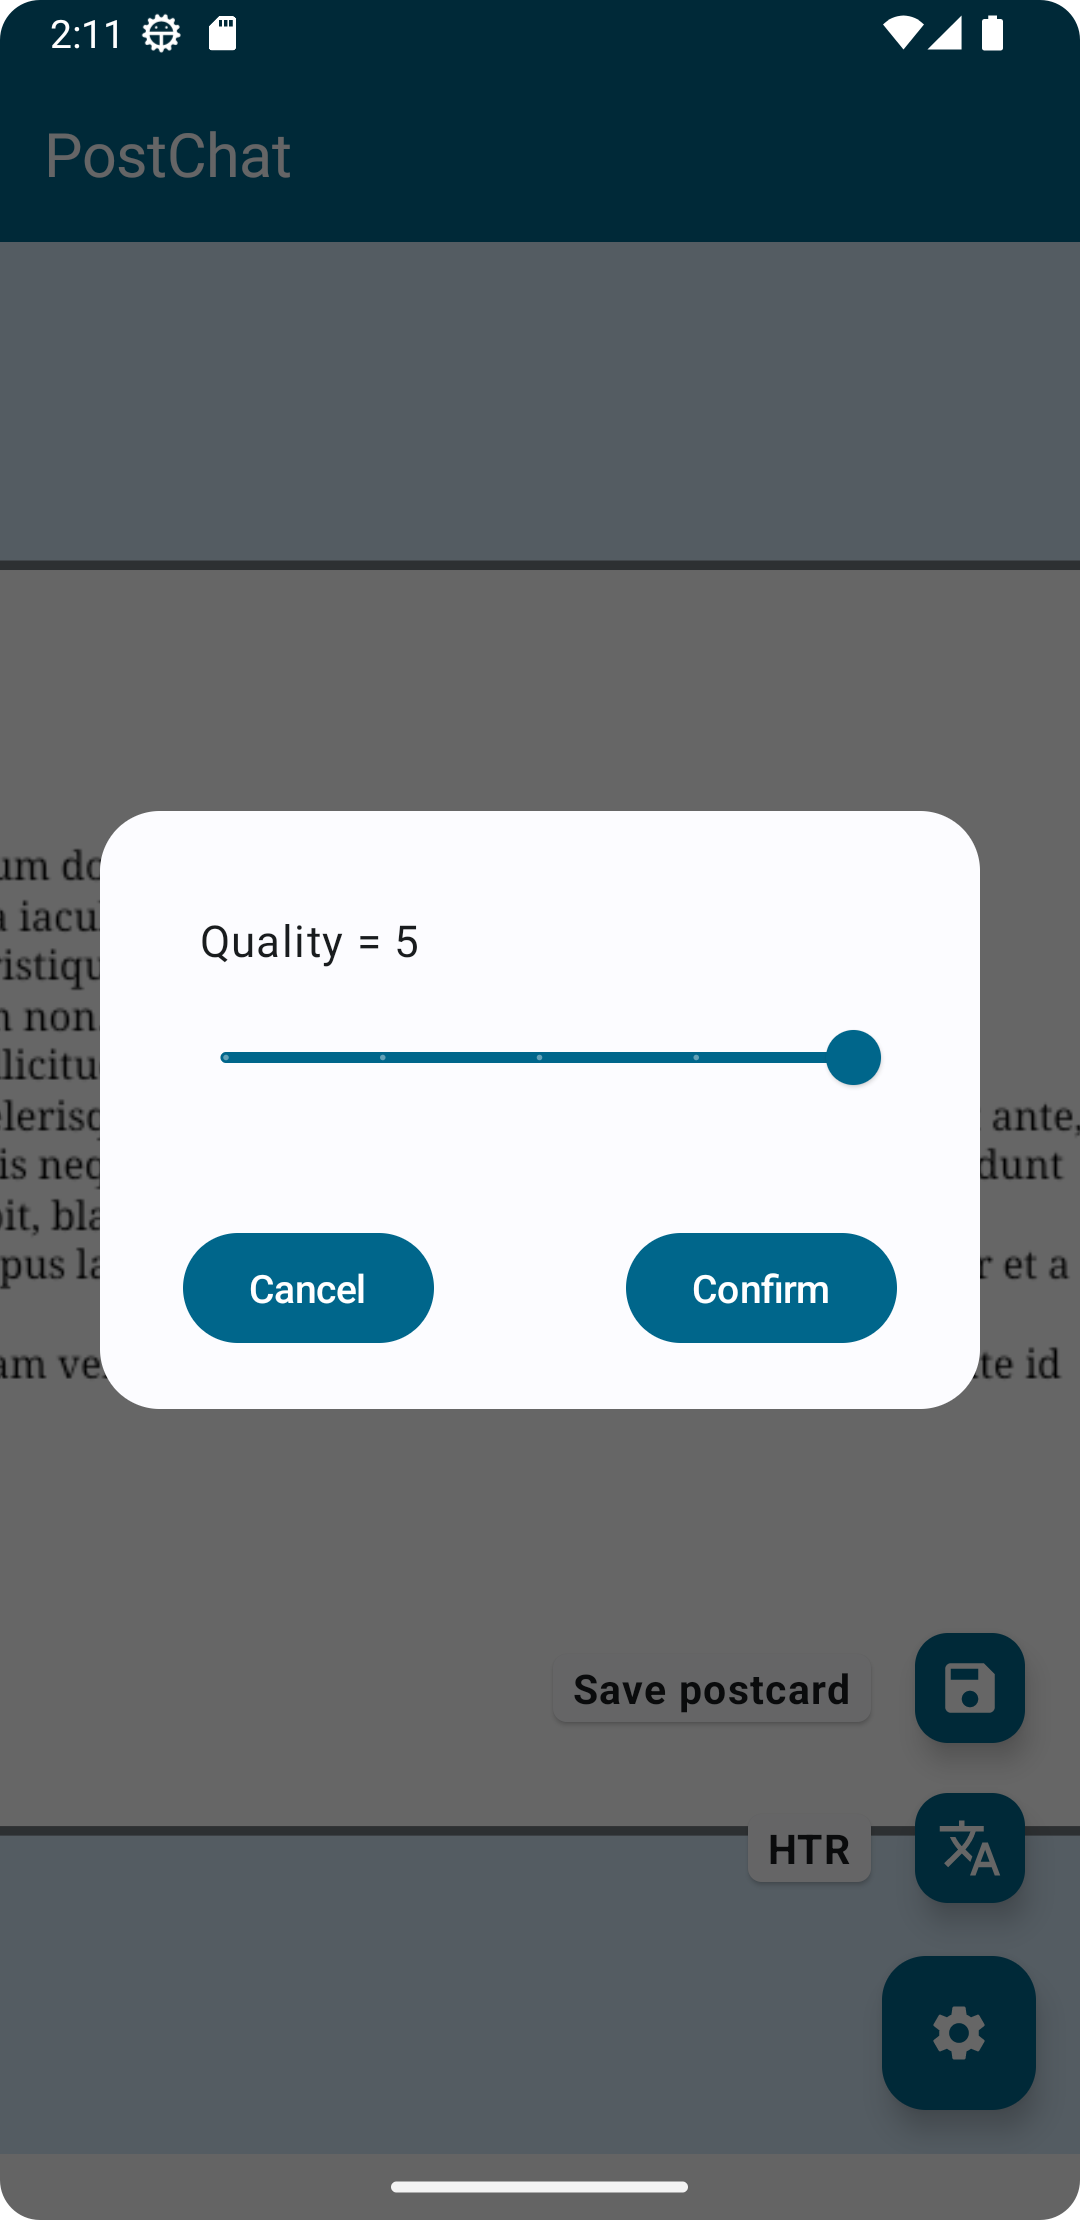
\includegraphics[trim={0cm -3cm 0 -3cm}, width=0.4\textwidth]{./Chapter6/Figures/PostcardActivitySave}
	\caption{Postcard save}
	\label{fig:VA1}
\end{figure}

\begin{figure}[!ht]
	\centering
	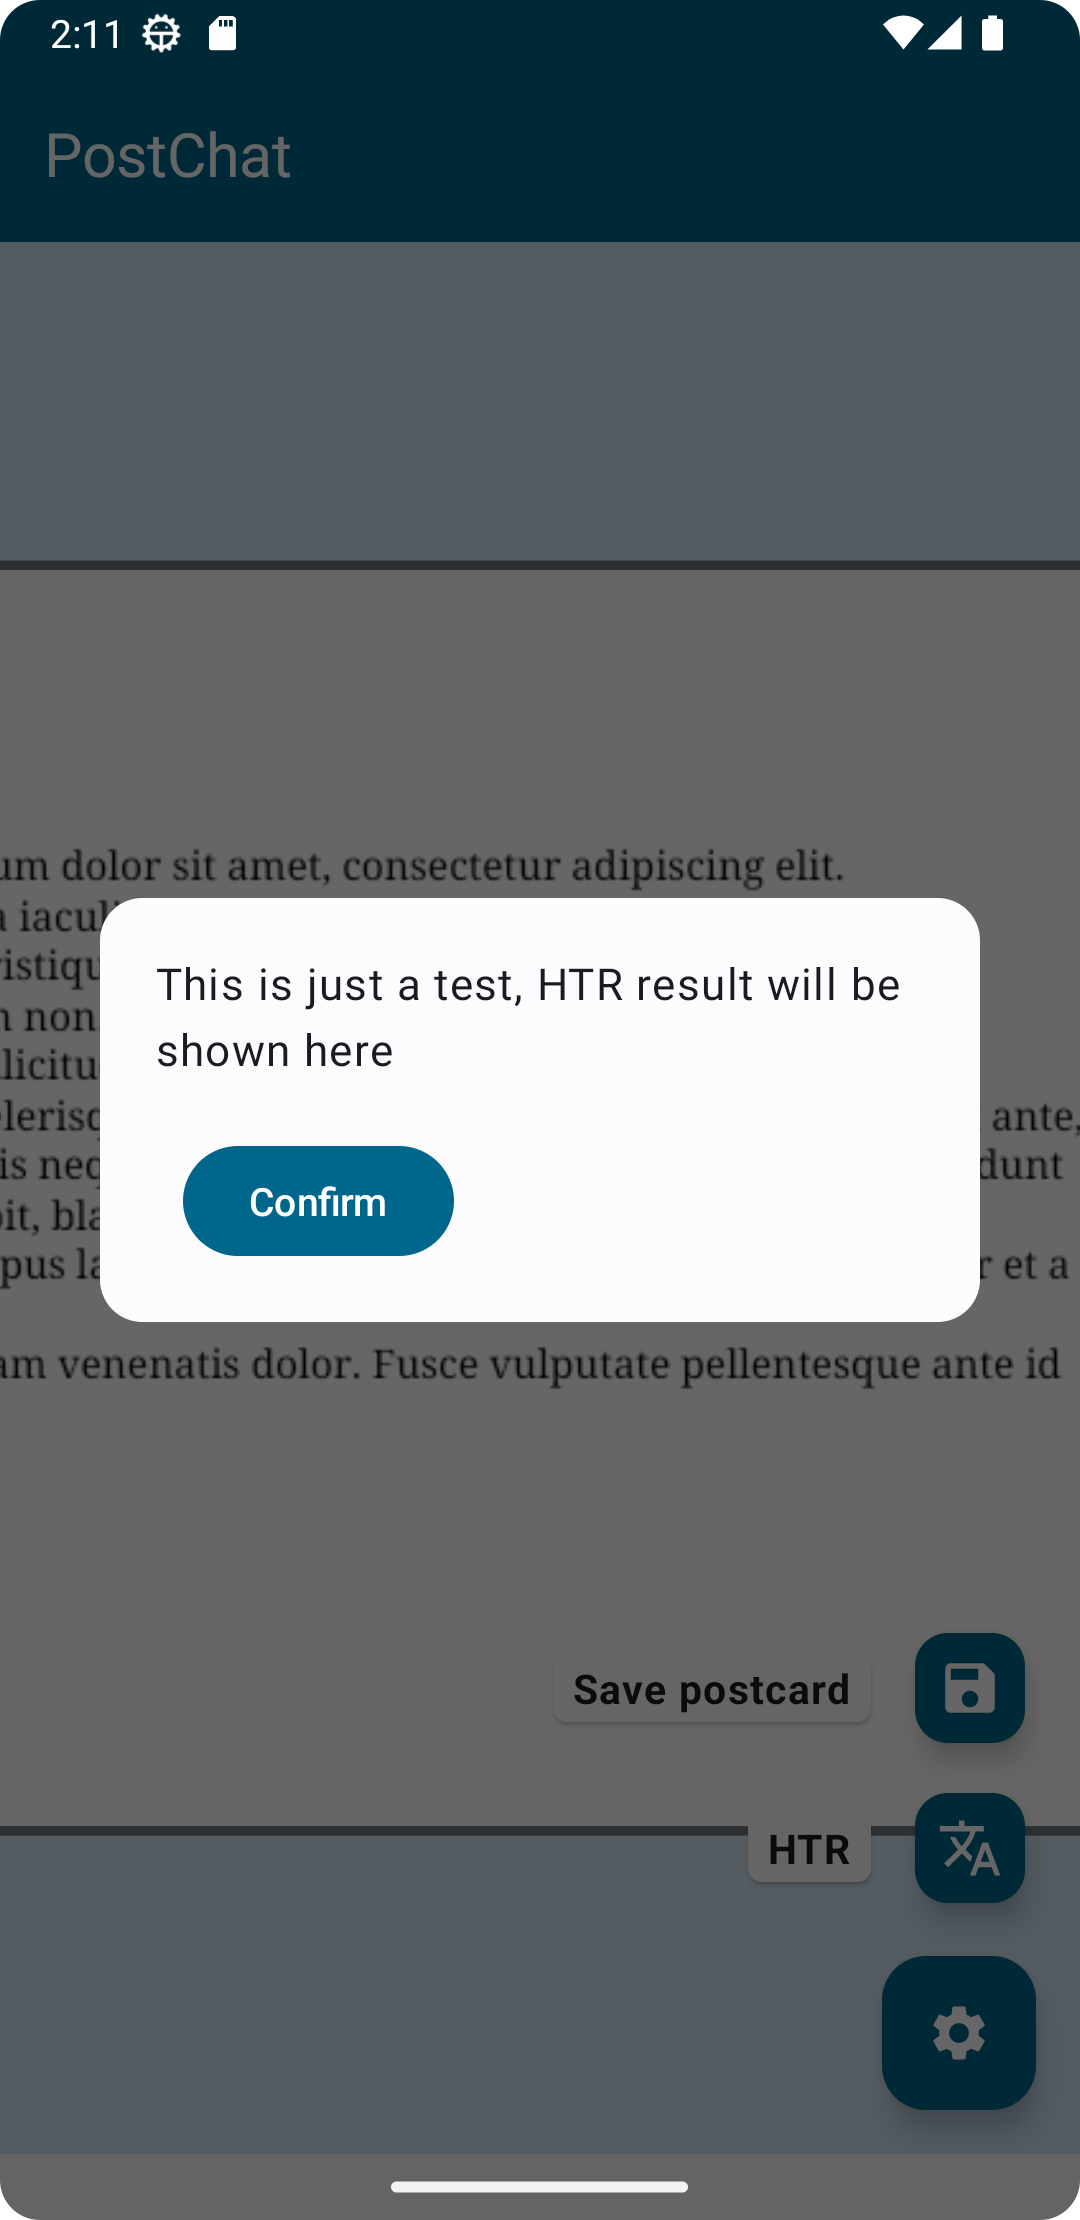
\includegraphics[trim={0cm -3cm 0 -3cm}, width=0.4\textwidth]{./Chapter6/Figures/PostcardActivityHTR}
	\caption{Postcard perform HTR}
	\label{fig:VA2}
\end{figure}


\subsection{Settings and Information}
The settings activity plays a major role in debugging but it is not limited to just that.

In this activity a user can delete its account or logout from the service.
Other settings are just for data visualization by the programmer and should be treated as so. They offer no utility for the final consumer and will be hidden from the same when ready for production.

There is a icon in the top right of the corner that leads to the activity containing information about the program and team behind it.

Figures \ref{fig:SIA} and \ref{fig:SIA1} illustrate the implemented activities.

\begin{figure}[!ht]
	\centering
	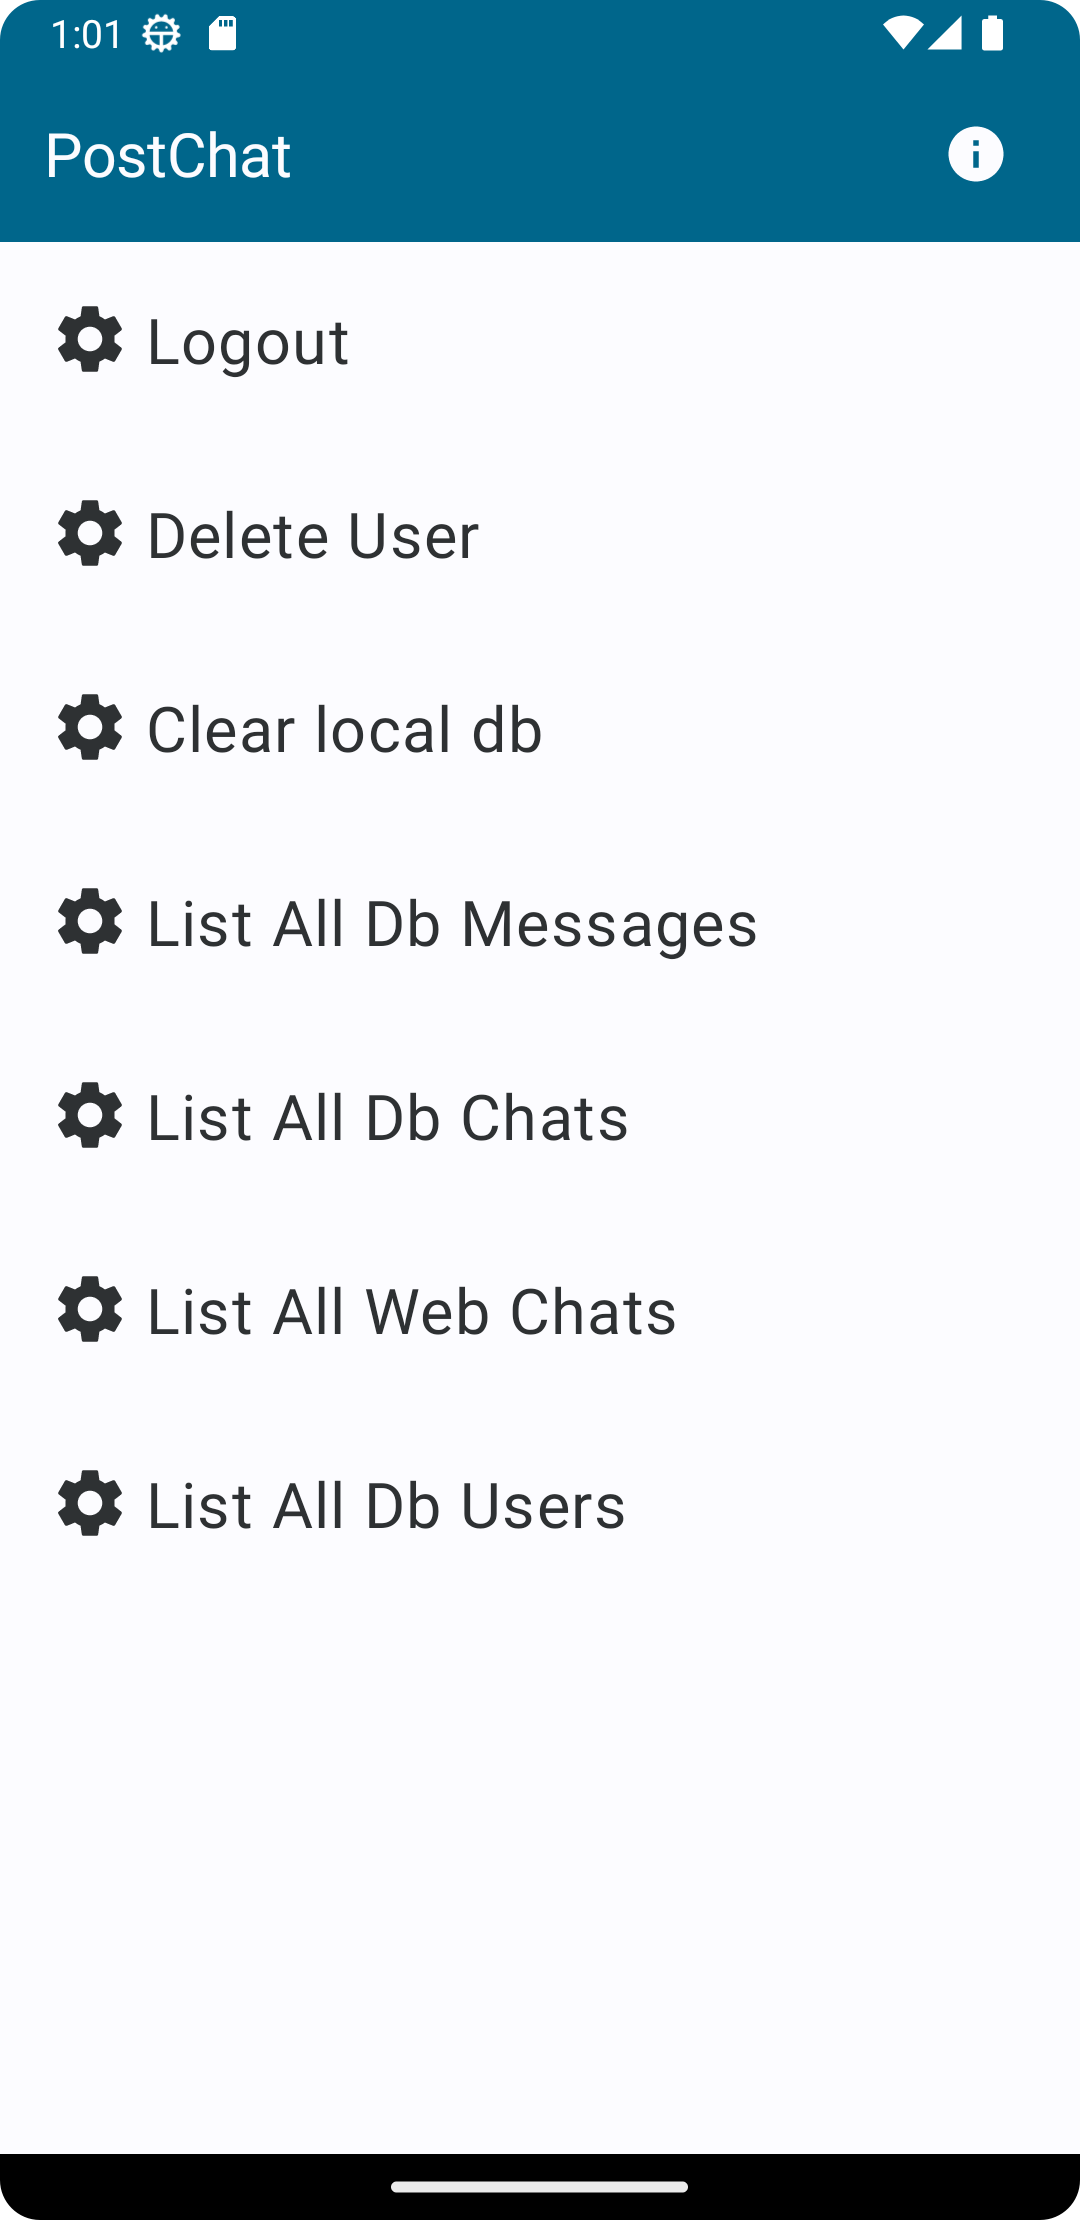
\includegraphics[trim={0cm -3cm 0 -3cm}, width=0.4\textwidth]{./Chapter6/Figures/SettingsActivity}
	\caption{Settings activity}
	\label{fig:SAI}
\end{figure}


\begin{figure}[!ht]
	\centering
	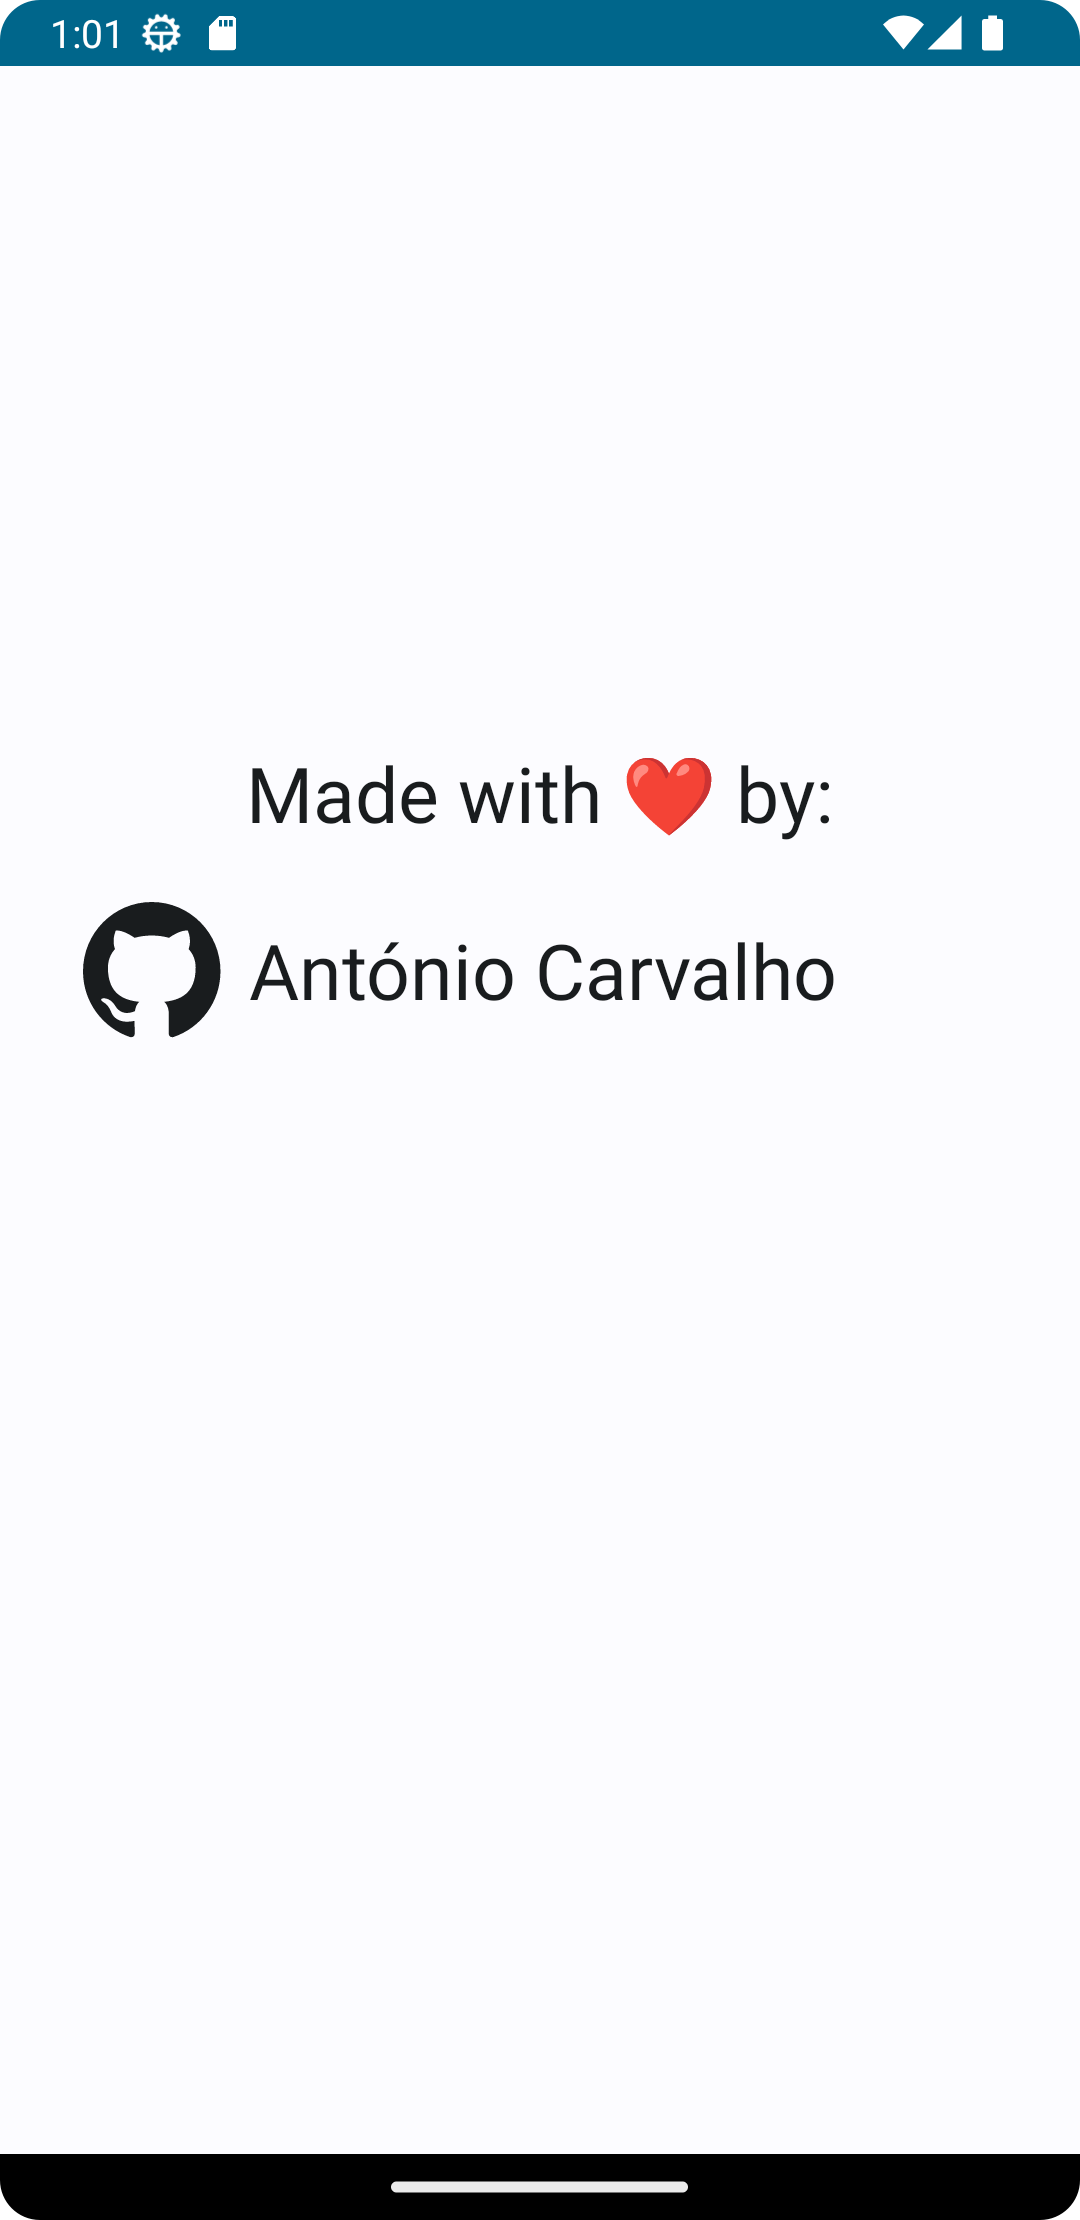
\includegraphics[trim={0cm -3cm 0 -3cm}, width=0.4\textwidth]{./Chapter6/Figures/InfoActivity}
	\caption{Information activity}
	\label{fig:SAI1}
\end{figure}






%////////////////////////////////////////////////////////////////////////
%   Chapter 7
%
%   
%////////////////////////////////////////////////////////////////////////
%\chapter{Accelerated Local Search Algorithms for Examination Timetabling} 
\label{ch:Chapter7}
\vfill \minitoc \newpage


The previous two chapters presented three memetic algorithms which combine evolutionary algorithms with local search. Three local search algorithms were employed, namely \gls{sa}~\citep{Kirkpatrick1983}, \gls{ta}~\citep{Dueck1990}, and \gls{gd}~\citep{Dueck1993}. In this chapter, we present an accelerated \gls{sa} local search algorithm, named \gls{fastSA}, and show its application on the \gls{etp}. The proposed framework of \gls{fastSA} was adapted to the \gls{ta} algorithm in~\cite{Leite2019a}.

Section~\ref{sec:ProposedApproach} presents the proposed simulated annealing variant developed for approaching the examination timetabling problem. Section~\ref{sec:ExperimentalResults} reports the experimental results on the \gls{itc2007} benchmark set and compare the FastSA's results with the ones in the literature. Section~\ref{sec:Conclusions} presents concluding remarks and future work.



%//////////////////////////////////////////////////
%
% Section 3
%
%//////////////////////////////////////////////////
\section{Proposed Approach}
\label{sec:ProposedApproach}

This section describes the proposed approach based on the SA metaheuristic, named \gls{fastSA}. Section~\ref{subsec:SolutionRepresentationAndConstructionOfInitialFeasibleTimetables} describes the solution representation and the process of constructing an initial and feasible solution.  Section~\ref{subsec:SABasedSearchMethod} describes the SA-based search method and the neighbourhood structure used. Finally, in Section~\ref{subsubsec:FastSA}, the \gls{fastSA} approach is explained.


%///////////////////////////////////////////////////
% Subsection
\subsection{Solution Representation and Initial Solution Construction} 
\label{subsec:SolutionRepresentationAndConstructionOfInitialFeasibleTimetables}

Each solution manipulated by the search method encodes a complete and feasible timetable. The adopted solution representation is described in Section~\ref{sec:Chapter6_ChromosomeRepresentation} and illustrated in Figure~\ref{fig:EncodingSchemeITC2007}. 


We now describe the process of constructing an initial and feasible solution. The proposed solution method only works with feasible solutions and thus it does not permit violations of hard constraints.

The construction method is an improved version of the method presented in Chapter~\ref{ch:Chapter6}. The initial solution is constructed using a variant of the \gls{sd} graph colouring heuristic~\citep{Brelaz1979,Cheong2009}. In the \gls{sd} heuristic, exams with the fewest valid periods, in terms of satisfying the hard constraints, remaining in the timetable are reinserted first~\citep{Cheong2009}. The \gls{sd} heuristic is implemented using a priority queue of the exams to be placed in the timetable. Each exam's priority is set to the exam's number of available periods. In the proposed approach, for performance reasons, the number of available periods of each exam is computed by considering only the \textit{After} hard constraint (in the initial phase), and the \textit{No Conflicts} (or clash) hard constraint, instead of considering all hard constraints. The remaining hard constraints are verified when the exam is scheduled. 

In order to schedule the more constrained exams first, the exams in the queue are initially sorted by decreasing order of their number of \textit{After} hard constraints. The other types of period related hard constraints (\textit{Exam Coincidence} and \textit{Period Exclusion}) are not considered in the initial exam sorting. The exams that must be placed before others (involved in an \textit{After} constraint) have fewer available periods, and are thus more difficult to schedule. The initial sorting is done as follows. The initial priority of each exam is set to the \textit{number of total periods}, $T$. Then, all the exams that must be scheduled before another exam have their number of feasible periods decremented by one, for each \textit{After} hard constraint in which are involved. For instance, if an exam $e_i$ must be scheduled \textit{before} exam $e_j$ (an \textit{After} constraint exists between $e_j$ and $e_i$), then the available periods for $e_i$ include all periods except the last period, in order to make room for $e_j$. Hence, the number of available periods for $e_i$ is equal to $T-1$, and the number of available periods for $e_j$ is equal to $T$. In this way, $e_i$ has more priority than $e_j$ and is scheduled first. 


The construction algorithm proceeds in two steps:
\begin{description}
	\item[Step 1] Extract an examination from the exam priority queue and, if all hard constraints are met, schedule the exam in the selected period and room, and update the priorities of exams placed in the queue, considering only the \textit{No Conflicts} hard constraint. Then, repeat the same process for the next maximum priority exam located in the queue. If a given exam cannot be scheduled, then go to Step 2. The construction phase ends when all exams are scheduled. 
	
	\item[Step 2] If a selected exam cannot be assigned due to violations of hard constraints with existing assignments, the conflicting exams are unscheduled and the selected exam is scheduled. The conflicting exams are again inserted in the exam priority queue. The priority of each exam in the queue is recomputed according to the \gls{sd} heuristic. Then, go to Step 1. 
	
	In order to prevent repetitive assignments of variables (exams) to the same values (period and room), the \gls{cbs}~\citep{Muller2009} data structure is used. \gls{cbs} is a data structure that stores \textit{hard conflicts} (violations of the hard constraints) which have occurred during the search, together with their frequency, and the assignments that caused them. In the (period, room) value selection, the value that has the lowest number of weighted hard conflicts is chosen. For a description of the \gls{cbs} data structure and its use in the construction of solutions please refer to~\citep{Muller2016}.
\end{description}



% Subsection
\subsection{Simulated Annealing-based Search Method}
\label{subsec:SABasedSearchMethod}

In the optimisation phase, a SA-based approach is applied. Two variants were implemented: the standard SA and an accelerated one, which was named \gls{fastSA}. The \gls{sa} metaheuristic and neighbourhood relation are explained in this section. We also describe the \gls{sa} parameter configuration adopted in order to satisfy the \gls{itc2007} rules. The FastSA is presented in Section~\ref{subsubsec:FastSA}.


\subsubsection{SA and Kempe Chain Neighbourhood}
\label{sec:KempeChainNeighbourhood}

The template of the standard \gls{sa} algorithm is described in Algorithm~\ref{alg:SA}. In the proposed approach, the \textit{Kempe chain} neighbourhood~\citep{Thompson1998} is used (see Section~\ref{subsec:Chapter2_KempeChainNeighbourhood}). In this work, we have used the same two neighbourhood operators, previously introduced in Section~\ref{sec:neighbourhoodOperatorITC2007}:
\begin{description}
	\item[Slot-Room move] -- A random exam is scheduled in a different period and room, both chosen randomly.
	
	\item[Room move] -- An exam, chosen randomly, is scheduled into a different room in the same period. The destination room is chosen in a random fashion.
\end{description}

Figure~\ref{fig:ITC2007KempeChain} illustrates the use of the \textit{Slot-Room move} operator on an example ITC 2007 solution. 



\subsubsection{SA Parameter Configurations and Cooling Rate Computation}
\label{subsubsec:CoolingRateComputation}

In this section some details about the specification of the SA parameters are given. According to the ITC 2007's rules, participants have to benchmark their machine with the programme provided by the organisation. This is done in order to know how much time the participants have available to run their programme on their machines~\citep{ITC2007}. In our case, the available algorithm computation time, determined by the  benchmarking tool provided by the ITC 2007, is 276 seconds. In the ITC 2007's rules it is also pointed out that the programmer should not set different parameters for different instances. However, if the computer programme is doing this automatically then this is acceptable.

In this work, two SA parameter configurations are specified, which are used in two different set of experiments. In the first SA parameter configuration, a distinct set of parameters is used for each ITC 2007 instance. To note that this parameter setting does not comply with the ITC 2007 requirements. However, this parameter configuration is only used in experiments involving proposed variants of the SA algorithm, and not in state-of-the-art algorithm comparison.

The second set of parameters used is in line with the ITC 2007 rules and comprises a fixed set of SA parameters for all instances, excepting the cooling rate value which is computed automatically by the proposed algorithm for each ITC 2007 instance. In previously published work~\citep{Nunes2015,Nunes2016} this same issue is addressed; the authors propose a SA metaheuristic in which the cooling rate parameter is computed automatically for each instance. The other SA parameters (initial and final temperatures, and number of iterations at a fixed temperature) remain constant for all benchmark instances. In the present work, a SA is proposed which follows the same ideas introduced in~\citep{Nunes2015,Nunes2016}.

Hence, a SA with a variable rate was implemented to make this metaheuristic run closer to the given ITC 2007 time limit for all ITC 2007 instances. In order to determine the proper cooling rate, the algorithm starts by simulating the execution of the SA metaheuristic, by running the local search neighbourhood operator $AverageReps$ times. For simplicity, instead of executing each complete step of the SA metaheuristic (generation and evaluation of the neighbour followed by the application of the acceptance criterion) only the generation and evaluation of the neighbour are performed. The $AverageReps$ parameter was set to \num{10000}. This value was found empirically to be adequate, allowing a reasonable number of runs to be performed while not taking too much computation time. Using the elapsed time and the given ITC 2007 time limit, the number of neighbours that would be generated if this heuristic was to be run within the time limit is estimated. The number of neighbours is computed using the expression 
\begin{linenomath*}
	\begin{equation}
	CompNeighbs = TotalTime / CompTime \cdot AverageReps, \label{eq:CompNeighbs}
	\end{equation}
\end{linenomath*}
where parameter $TotalTime$ denotes the ITC 2007 time limit (\num{276000} milliseconds), $CompTime$ denotes the elapsed time used in the simulation, and $AverageReps$ denotes the number of loops the local search neighbourhood operator was run (\num{10000} runs). After that, the exact number of neighbours ($TotalNeighbs$) that will be generated for the given SA parameters, using an initial default rate, is computed. This initial rate is subsequently adjusted by the algorithm until $TotalNeighbs$ is sufficiently close to the $CompNeighbs$ value. Algorithm~\ref{alg:RateComputation} describes the pseudocode of the algorithm used to compute the SA cooling rate in an automatic fashion.


\afterpage{%
	%	\clearpage% Flush earlier floats
	\begin{algorithm}[!ht]
		\textbf{Input:} 
		\begin{itemize}
			\setlength{\itemsep}{1pt}
			\item $s$ \Comment{Solution}
			\item $T_{Max}$ \Comment{Maximum temperature}
			\item $T_{Min}$ \Comment{Minimum temperature}
			\item $reps$ \Comment{Number of iterations per temperature}
			\item $exec\_time$ \Comment{ITC 2007 time limit}
		\end{itemize}
		\begin{algorithmic}[1]
			\State $n \leftarrow \num{10000}$  \Comment{Number of neighbourhood operator runs}
			\State $comp\_neighbours \leftarrow estimateNumberNeighbours(n, exec\_time, s)$ 
			\State $offset \leftarrow  0.8$
			\State $comp\_neighbours \leftarrow comp\_neighbours \cdot  offset$
			\State $rate \leftarrow \num{1e-3}$ \Comment{Initial default rate}
			\State $rate\_to\_sub \leftarrow \num{1e-3}$ \Comment{Rate subtraction factor}
			\State $depth \leftarrow 3$ \Comment{Number of iterations until convergence}
			\While { $depth > 0$ } 
			\State $total\_neighbours \leftarrow getSANumberNeighbours(T_{Max}, rate, reps, T_{Min})$
			\If { $total\_neighbours < comp\_neighbours$ }
			\If { $rate <= rate\_to\_sub$ }
			\State $rate\_to\_sub \leftarrow rate\_to\_sub / 10$
			\EndIf
			\State $rate \leftarrow rate - rate\_to\_sub$
			\Else
			\State $rate \leftarrow rate + rate\_to\_sub$ \LONGCOMMENTTWO{To guarantee that total\_neighbours $<$ comp\_neighbours}
			\State $depth \leftarrow  depth - 1$
			\State $rate\_to\_sub \leftarrow rate\_to\_sub / 10$
			\EndIf
			\EndWhile
			\State \textbf{Output:} $rate$ \Comment{Return computed rate}
		\end{algorithmic}
		\caption{SA cooling schedule rate computation.}
		\label{alg:RateComputation}
	\end{algorithm}
%	\clearpage% Flush page
}


The calculation represented in~\eqref{eq:CompNeighbs} is done in line 2 of Algorithm~\ref{alg:RateComputation} by the function $estimateNumberNeighbours$. In lines 3--4, an \textit{offset} term is used in the computation of $comp\_neighbours$. This offset represents the percentage of $comp\_neighbours$ to be considered in the rate computation. The use of a percentage is justified by the process used in the computation of the $comp\_neighbours$ parameter value, which does not take into account all the steps of the SA metaheuristic, and also by the stochastic nature of the SA. It was verified experimentally that for some instances the given time limit was exceeded, and for other instances the computation time was below the time limit. In the proposed FastSA approach (Section~\ref{subsubsec:FastSA}), the computation times differences to the ITC 2007 time limit were even more noticeable, as documented in Section~\ref{sec:ExperimentalResults}. The offset used is 80\%. In lines 7--20 of Algorithm~\ref{alg:RateComputation}, the $rate$ parameter is iteratively adjusted until the number of computed neighbours for the chosen SA parameters, i.e. $total\_neighbours$, is close and less than the theoretical value of $comp\_neighbours$. Function $getSANumberNeighbours$ returns the SA number of neighbours, or number of evaluations done, for the given parameters.

Some experiments were made in order to check Algorithm~\ref{alg:RateComputation}'s behaviour, for ITC 2007's Instance 4, using the following parameters: $T_{Max} = 0.01$, $T_{Min} = \num{1e-06}$, $reps = 5$, $exec\_time = \num{276000}$ ms, and computed $rate = \num{6.8e-06}$ (rate computed automatically using Algorithm~\ref{alg:RateComputation}). For the given parameters, the computed neighbours $comp\_neighbours \cdot offset$ is $\num{6773005}$, whereas the number of evaluations ($total\_neighbours$) is $\num{6772311}$. The elapsed computation time was $\num{219000}$ ms. 

Figure~\ref{fig:SimulatedAnnealingPlot} illustrates the solution fitness evolution for ITC 2007's Instance 4 when applying SA with the above parameters. The $x$-axis represents the number of generated feasible neighbours, and the $y$-axis represents the solution fitness. As can be seen in Figure~\ref{fig:SimulatedAnnealingPlot}, SA starts by accepting some worse and better neighbour solutions. In the end, the temperature is so low that it becomes harder to accept worse solutions, ending up acting similar to the \textit{hill-climbing} procedure. 


%%%%%%%%%%%%%%%%%%%%%%%%%%%%%%%%%%%%%%%%%%%%%%%%%%%%5
%-
% Figure 3 
%-
%\afterpage{%
%	\clearpage% Flush earlier floats
\begin{figure}[H]
	\centering
	\hspace*{-1em}
	\scalebox{0.85}{\includegraphics{./Chapter7/Figures/FIG_3_SA_Plot_Instance_4_crop.pdf}}
	
	\caption{Solution fitness evolution for ITC 2007's Instance 4 when applying simulated annealing.} 
	\label{fig:SimulatedAnnealingPlot}
\end{figure}
%\clearpage% Flush page
%}


In this experiment, the number of generated \textit{feasible} neighbours was \num{3143070} ($\approx 46.41\%$ of $total\_neighbours$), whereas the number of accepted neighbours (the maximum number of iterations in Figure~\ref{fig:SimulatedAnnealingPlot}) was $\num{48837}$, which is  $\approx 1.55\%$ of the number of accepted neighbours. These numbers show that it is difficult to generate feasible neighbours with the Kempe chain move and also that the SA initial temperature has a relatively low value, resulting in a low percentage of accepted neighbours. Despite this, the SA is able to obtain a relatively good final solution fitness value.





%/////////////////////////////////////////////////////////////

\subsection{Accelerating the SA Metaheuristic for the ETP}
\label{subsubsec:FastSA}

In this section, the FastSA search method for solving the ETP is explained. In the first subsection, the effect of the cooling schedule on the exam move acceptance rate in SA-based algorithms is studied, introducing the basic framework used by the FastSA method. This study extends the study previously made on Section~\ref{sec:Chapter6_LocalSearchEffect} for the \gls{ta} applied to the Toronto benchmark set. 

The FastSA approach is described in the second subsection. 


\subsubsection{Effect of the Cooling Schedule on the Exam Move Acceptance Rate}
\label{subsubsec:LocalSearchEffect}

In the study carried out in this section, the effect of the cooling schedule on the exam move acceptance in SA-based algorithms is analysed. Some important properties of the local search operator are identified, which are exploited by the FastSA algorithm.

In the experiments, two different cooling schedules were used: a \textit{light} cooling schedule, with parameters $T_{max} = 0.1$ (initial temperature),  $r =  \num{1e-4}$ (decreasing rate), $k = 5$ (\# iterations at each temperature), and $T_{min} = \num{1e-7}$ (final temperature); and an \textit{intensive} cooling schedule, with parameters $T_{max} = 0.1$, $r =  \num{1e-5}$, $k = 5$, and $T_{min} = \num{1e-7}$. With the light cooling schedule, each SA algorithm execution computes \num{690780} evaluations. With the intensive cooling schedule,  \num{6907760} evaluations are computed by each SA algorithm execution. The justification for the choice of the SA parameters is given at the end of this section.




%
% Color figures
%

%%%%%%%%%%%%%%%%%%%%%%%%%%%%%%%%%%%%%%%%%%%%%%%%%%%%5
%-
% Figure 4 
%-
\afterpage{%
	%%	\clearpage% Flush earlier floats
	\begin{figure}[H]
		\centering
		\scalebox{0.7}{\includegraphics{./Chapter7/Figures/FIG_4_dataset4_Cool1Eminus4_Cool1Eminus5_crop.pdf}}
		
		\caption{Study of the effect of applying \textit{light} and \textit{intensive} cooling schedules in the SA algorithm for ITC 2007's Instance 4: (a) optimisation using the \textit{light} cooling schedule (obtained cost: \num{14058}); (b) optimisation using the \textit{intensive} cooling schedule (obtained cost: \num{12528}). The figure shows the evolution of the number of accepted exam moves, for each exam in the $y$-axis, per each temperature bin. The exams in the $y$-axis are sorted by decreasing order of number of conflicts with other exams. The marked $x$-axis long ticks represent the temperature intervals.}
		
		\label{fig:LocalSearchStudyDataset4} 
	\end{figure}
	%\clearpage% Flush page
}



%%%%%%%%%%%%%%%%%%%%%%%%%%%%%%%%%%%%%%%%%%%%
%-
% Figure 5 
%-
\afterpage{%
	%	\clearpage% Flush earlier floats
	\begin{figure}[H]
		\centering
		\scalebox{0.7}{\includegraphics{./Chapter7/Figures/FIG_5_dataset9_Cool1Eminus4_Cool1Eminus5_crop.pdf}}
		
		\caption{(continuation). Study of the effect of applying \textit{light} and \textit{intensive} cooling schedules in the SA algorithm for ITC 2007's Instance 9: (a) optimisation using the \textit{light} cooling schedule (obtained cost: \num{1243}); (b) optimisation using the \textit{intensive} cooling schedule (obtained cost: \num{1024}).}
		
		\label{fig:LocalSearchStudyDataset9} 
	\end{figure}
	%\clearpage% Flush page
}
%%%%%%%%%%%%%%%%%%%%%%%%%%%%%%%%%%%%%%%%%%%%

Figures~\ref{fig:LocalSearchStudyDataset4} and~\ref{fig:LocalSearchStudyDataset9} illustrate the evolution of the number of accepted exam movements as the SA temperature varies, for two example ITC 2007 instances. In these figures, the x-axis value range is divided into ten \textit{temperature bins}. A \textit{temperature bin} corresponds to a temperature interval and is represented by two vertical grid lines, interpreted from the x-axis in the figures.


The temperature bins were calculated in order for the SA metaheuristic to compute, in each bin, 1/10 of the total number of evaluations. The colour codes represented in each bin, and for each exam on the y-axis, represent the number of accepted movements for the corresponding exam. The total number of exams' accepted moves per bin is generally lower than the number of evaluations performed in that bin, as not all the exams are subject to an accepted move in each local search move. Some exams do not move because the fitness difference violates the SA acceptance criterion, or are not selected by the neighbourhood operator. The exams are ordered decreasingly by the number of conflicts they have with other events (\textit{largest degree} heuristic~\citep{Cheong2009}).

It can be observed that the more difficult exams (the ones with lower indexes) only move (a move is accepted by the SA) when higher temperatures are applied, being gradually fixed at the same timeslot when lower temperatures are applied (e.g., below temperature \num{1e-2}). The easier exams (those with higher indexes) continue to move, being gradually arranged in their definitive place. 

As it can be seen from the difference in the top and bottom plots from Figures~\ref{fig:LocalSearchStudyDataset4} and~\ref{fig:LocalSearchStudyDataset9} (and corresponding solutions' fitness), it is essential that the difficult exams be well arranged, in an optimal or near optimal place, for the easier exams also to be placed in an optimal fashion. If a cooling schedule with few evaluations is used, the SA algorithm cannot find the optimal (near optimal) place for the difficult exams and so the easier exams are also placed in a suboptimal way. 

For this experiment, the SA parameters were set as follows. We have selected an initial temperature value that allows for the great majority of exams to be moved several times, in order to better explore the search space. Graphically, we know that this effect is achieved by having the first temperature bin practically filled in Figures~\ref{fig:LocalSearchStudyDataset4} and~\ref{fig:LocalSearchStudyDataset9}. After several experiments we have determined that the value $T_{max}=0.1$ was a reasonable value. The remaining parameters of the cooling schedule ($r$, $k$, and $T_{min}$) were set in order to have two distinct rates (parameter $r$), a \textit{light} one and an \textit{intensive} one, a low number of iterations at a fixed temperature (parameter $k$) since the intensification is mainly controlled by the rate parameter, and a sufficiently low temperature ($T_{min}$ parameter), that is, a value from which non-improving moves are practically never accepted.





\subsubsection{FastSA Search Method for the ETP}
\label{sec:FastSASearchMethod}

As it can be observed from Figures~\ref{fig:LocalSearchStudyDataset4} and~\ref{fig:LocalSearchStudyDataset9}, several of the more difficult exams are going to be fixed (or have few moves) as lower temperatures are reached. In the algorithm, if it were decided not to move (and not evaluate the corresponding movement) an exam having zero or few movements in the previous temperature bin, it would produce a faster SA algorithm. The faster execution comes at the expense of a degradation of the results, if there exist bins with exam movements followed or interleaved with bins with no movements, because the algorithm would stop evaluating moves for a given exam when a bin with zero moves is found. This faster SA variant was implemented in this work, and was named FastSA. The template of the FastSA algorithm is given in Algorithm~\ref{alg:FastSA}. 

\afterpage{%
	%	\clearpage% Flush earlier floats
	\begin{algorithm}[H]
		\textbf{Input:} Cooling schedule.
		\begin{algorithmic}[1]
			\boldnext		
			\State $prevBin \leftarrow $ nil; \Comment Array containing \# accepted moves in the previous bin, initially nil
			\boldnext
			\State $currBin \leftarrow $ createArray(numExams); \Comment Array containing \# accepted moves in the current bin, initialised with zeros
			\State $s \leftarrow s_0$; \Comment Generation of the initial solution
			\State  $T \leftarrow T_{max}$; \Comment Starting temperature
			\Repeat
			\Repeat \Comment At a fixed temperature 
			\State Generate a random neighbour $s' \in N(s)$;
			\boldnext
			\State $examToMove \leftarrow$ selectExamFromSolution$(s')$
			\boldnext
			\If{ $prevBin = $ nil or ($prevBin <> $ nil and $prevBin\left[examToMove\right] > 0$)} \Comment Evaluate neighbour solution 
			\State $\Delta f \leftarrow \frac{f(s') - f(s)}{f(s)}$ \Comment Relative change in cost between $f(s')$ and $f(s)$
			\label{algline:acceptanceRuleBegin1}
			\If{ $\Delta f \leq 0$} 
			{$s \leftarrow s'$} \Comment Accept the neighbour solution 	
			\Else 
			{ Accept $s'$ with a probability $e^{\frac{- \Delta f}{T}}$; }
			\EndIf \label{algline:acceptanceRuleEnd1}
			\boldnext
			\If{ $s'$ was accepted }
			\boldnext
			\State $currBin\left[examToMove\right] \leftarrow currBin\left[examToMove\right] + 1$
			\boldnext
			\EndIf
			\boldnext
			\EndIf	
			\Until Equilibrium condition
			\LONGCOMMENTONE{e.g., a given number of iterations executed at each temperature $T$}
			\State $T \leftarrow g(T)$; \Comment temperature update 
			\boldnext
			\State $prevBin \leftarrow \text{updateBin}(T, currBin)$ \Comment If $T$ is in the next bin, make $prevBin \leftarrow currBin$ and zero $currBin$ 
			\Until Stopping criteria satisfied \Comment e.g., $T < T_{min}$ 
			\State \textbf{Output:} Best solution found.
		\end{algorithmic}
		\caption{Template of the \textit{fast simulated annealing} algorithm.}
		\label{alg:FastSA}
	\end{algorithm}
	%\clearpage% Flush page
}


The lines with numbers marked in bold are lines that were added to the original SA algorithm (Algorithm~\ref{alg:SA}). The FastSA keeps a record of all successful neighbourhood movements taken in a given bin. When performing a neighbourhood movement, a random exam is selected and the algorithm first checks if there were any movements, for the exam to be moved, in the previous bin. If there was no previous movement for the candidate exam, then the current movement is not performed and not evaluated. With this strategy, the FastSA is able to attain a reduced number of evaluations compared to the standard SA. The cost degradation attained by the FastSA compared to the SA is not significant, as shown in the experimental evaluation carried out in Section~\ref{sec:ExperimentalResults}.


Example~\ref{example:FastSAExample} illustrates a simple example of the bin structure used by the FastSA. 


%%%%%%%%%%%%%%%%%%%%%%%%%%%%%%%%%%%%%%%%%%%%
%
% Color Figures
%
%
%-
% Figure 6
%-
\afterpage{%
	%	\clearpage% Flush earlier floats
	\begin{figure}[H]
		\centering
		\subfigure[]{ \label{fig:FastSABinsSubfigA}
			\centering
			\scalebox{0.84}{\includegraphics{./Chapter7/Figures/FIG_6_A_crop.pdf}}
		}
		\subfigure[]{ \label{fig:FastSABinsSubfigB}
			\centering
			\scalebox{0.71}{\includegraphics{./Chapter7/Figures/FIG_6_B_FastSAExample_crop.pdf}}
		}  
		
		\caption{Different representations of the bin structure used by the FastSA. Six examinations and four bins were considered: (a) number of times each exam is selected in each bin, (b) graphical representation of the data in (a) using a colour map.} 
		
		\label{fig:FastSABins} 
	\end{figure}
	%\clearpage% Flush page
}
%%%%%%%%%%%%%%%%%%%%%%%%%%%%%%%%%%%%%%%%%%%%%



\begin{exmp}
	\label{example:FastSAExample}
	
	This example uses synthetic data to show the bin structure used by the FastSA. Six examinations and four bins were considered. Figure~\ref{fig:FastSABinsSubfigA} illustrates the number of times each exam is selected in each bin. Figure~\ref{fig:FastSABinsSubfigB} gives a graphical representation of the same data using a colour map.
	
	When the FastSA is run using this data, the following behaviour is registered. Because exam $e_1$ was never selected in bin $b_2$, $e_1$ remains fixed (a move involving this exam is not evaluated) from bin $b_3$ onwards, even if it had a positive number of selections in bins $b_3$ and  $b_4$. Using the same reasoning, exams $e_2$, $e_3$, and $e_4$, remain fixed from bin $b_4$ onwards. Note the case of exam  $e_4$ which is selected in bin $b_4$ (marked in shaded grey). As the number of movements in the previous bin ($b_3$) is zero, $e_4$ will be  fixed from bin $b_4$ onwards, and the three selections in bin $b_4$ are not evaluated by the FastSA, yielding a faster algorithm.
\end{exmp}








%//////////////////////////////////////////////////
%
% Section 4
%
%//////////////////////////////////////////////////
\section{Experimental Results and Discussion}
\label{sec:ExperimentalResults}

This section presents the experimental simulations conducted to test the proposed method in addressing the examination timetabling problem. Section~\ref{subsec:Settings} describes the experiments' settings and algorithm parameter settings. Section~\ref{subsec:ComparisonBetweenSAandFastSA} presents a comparison between three algorithms: two FastSA variants, named FastSA100 and FastSA80, and the standard SA. The FastSA100 variant is further compared with state-of-the-art approaches in Section~\ref{subsec:ComparisonStateOfTheArt}.



%////////////////////////////////////////////////////////
%=
% Subsection
%=
\subsection{Settings}
\label{subsec:Settings}

\noindent The developed algorithms were programmed in the C++ language using the ParadisEO framework~\citep{Talbi2009}. The hardware and software specifications are: Intel Core i7-2630QM, CPU @ 2.00 GHz $\times$ 8, with 8 GB RAM; OS: Ubuntu 16.10, 64 bit; Compiler used: GCC v. 4.8.2. The algorithm computation time was set to 276 seconds, as measured by the provided benchmarking tool from the ITC 2007 site~\citep{ITC2007} (please refer to Section~\ref{subsubsec:CoolingRateComputation} for more details). 


\subsubsection{Parameter Settings}
\label{subsubsect:ParameterSettings}

As mentioned in Section~\ref{subsubsec:CoolingRateComputation}, two parameter configurations were used in the conducted experiments. In the first configuration, the parameters were manually tuned for each ITC 2007 instance. This configuration was only used in the FastSA variants' comparison. In the second configuration, a fixed set of parameters was used for all instances, excepting the cooling rate, which was computed automatically by the optimisation algorithm. The second parameter configuration was used to compare the FastSA100 with the state-of-the-art approaches.

Table~\ref{tab:coolingSchedules} summarises the cooling schedule parameters used in the first configuration. The parameter values were chosen using as reference the FastSA100 algorithm (described in the next section). Specifically, the cooling schedule values were adapted empirically for each dataset instance, while guaranteeing that the FastSA100 computation time was within the ITC 2007 time limit constraint. 


%-
% TABLE_2.tex
%-
\begin{table}[!ht]
	\centering
	\caption{Cooling schedules used to solve the different ITC 2007 instances. The value presented in the bottom row, rightmost column, corresponds to the sum of the \# evaluations. The cooling schedule values were adapted empirically for each dataset instance using as reference the FastSA100 algorithm. \vspace{0.3em}}
	
	\sisetup{table-alignment=center,detect-weight=true,detect-inline-weight=math}
	\begin{tabular}{%
			S[table-format=2.0]% int
			S[table-format=2.3]%
			S[table-format=2.7]%    
			S[table-format=2.0]% int
			S[table-format=2.8]%    
			S[table-format=10.0]% int
		}
		
		\toprule
		
		\multicolumn{1}{l}{Inst.} 
		& \multicolumn{1}{c}{$T_{Max}$} 
		& \multicolumn{1}{c}{$rate$} 
		& \multicolumn{1}{c}{$k$} 
		& \multicolumn{1}{c}{$T_{Min}$}
		& \multicolumn{1}{c}{\# evaluations}\\%
		
		\midrule
		%Cooling schedules                                   
		%Inst. &  Tmax    &   rate    &   k   &   Tmin    &   Max evals   \\
		1   &   0.01    &   0.000003    &   5   &   \num{1.00E-06}      &   15350571    \\
		2   &   0.01    &   0.000004    &   5   &   \num{1.00E-06}      &   11512931    \\
		3   &   0.01    &   0.000005    &   4   &   \num{1.00E-06}      &   7368277     \\
		4   &   0.1     &   0.000005    &   6   &   \num{1.00E-06}      &   13815517    \\
		5   &   0.01    &   0.000007    &   6   &   \num{1.00E-06}      &   7894579     \\
		6   &   0.002   &   0.000003    &   5   &   \num{1.00E-06}      &   12668176    \\
		7   &   0.001   &   0.000003    &   5   &   \num{1.00E-06}      &   11512931    \\
		8   &   0.001   &   0.0000015   &   5   &   \num{1.00E-06}      &   23025856    \\
		9   &   0.01    &   0.000001    &   5   &   \num{1.00E-06}      &   46051706    \\
		10  &   0.01    &   0.000001    &   5   &   \num{5.00E-06}      &   38004516    \\
		11  &   0.01    &   0.000009    &   5   &   \num{1.00E-06}      &   5116861     \\
		12  &   0.01    &   0.0000013   &   5   &   \num{1.00E-06}      &   35424391    \\ 
		\midrule
		&           &               &       &   \text{$\sum$} &   227746312   \\
		
		\bottomrule
		
	\end{tabular}
	\label{tab:coolingSchedules}
\end{table}



For the second parameter configuration, the following parameter set was used: $T_{Max} = 0.01$, $T_{Min} = \num{1e-06}$, $reps = 5$, and $rate$ computed automatically using Algorithm~\ref{alg:RateComputation}.


The neighbourhood operators, the \textit{Room} and \textit{Slot-Room} moves, were selected with equal probability. This value was found after conducting some tuning experiments. Three runs of each ITC 2007 instance were executed, varying the probabilities values $(P_{sr}, P_{r})$ in the set: $\{ (0,1), (0.25, 0.75), (0.5,0.5),$ $(0.75,0.25), (1,0)\}$. $P_{sr}$ and $P_{r}$ denote, respectively, the probabilities of choosing the \textit{Slot-Room} and \textit{Room} moves. Selecting only the \textit{Room} move lead to the worse results, as only the room is changed. Triggering only the \textit{Slot-Room} move gives good results but slightly worse results in some instances compared to using both operators. No significant distinction was found using both operators  with the remaining probabilities combinations.


To obtain our simulation results, each algorithm was run ten times on each instance with different random seeds. In the experiments, all the statistical tests were performed with a 95\% confidence level. The developed source code, the resulting solution files for each instance/run, and the produced statistics, are publicly available on the following Git repository: \url{https://github.com/nunocsleite/FastSA-ETP-ITC2007}.





%////////////////////////////////////////////////////////
%=
% Subsection
%=
\subsection{Comparison between FastSA and SA Approaches}
\label{subsec:ComparisonBetweenSAandFastSA}

In this section, three algorithms, described as follows, were compared: 
\begin{enumerate}
	\item SA -- The original SA metaheuristic as described in Algorithm~\ref{alg:SA}.
	
	\item FastSA100 -- The basic FastSA algorithm as described in Algorithm~\ref{alg:FastSA}. In this approach, the exam movements in each bin are recorded, and if, for a selected exam, the number of movements in the previous bin is zero, that exam is \textit{fixed} until the end of the optimisation phase. This means that the current and future movements of this exam are not considered and thus not evaluated.
	
	\item FastSA80 -- In this variant, the behaviour is similar to the FastSA100 but the selected exam is fixed only if two conditions hold: the number of movements in the previous bin is zero \textit{and the exam belongs to the set comprising 80\% of the exams with the highest degree}. Observing again Figures~\ref{fig:LocalSearchStudyDataset4} and~\ref{fig:LocalSearchStudyDataset9}, we can see that the highest degree exams are those having the lower indices (top indices in the $y$-axis); on the other side, the lowest degree exams are the ones having the higher indices (the bottom ones in the $y$-axis). For the mentioned set of largest degree exams, the behaviour is the same as described for the FastSA100; for the remaining 20\% of the exams, the method behaves like the original SA, that is, the selected exam is never fixed and its move is always evaluated. The reasoning behind this variant is the following: because the lowest degree exams have a low number of conflicts with other exams, their moves imply a small change in the objective function; this, in turn, imply that they are likely to move more often than the higher degree exams, because small changes in the objective function are often accepted by the SA acceptance criterion, even at low temperatures. Hence, in the scenario that a lowest degree exam has no accepted moves in a previous bin, it is likely that it will have accepted moves in the future. With the FastSA80, the moves of the set comprising 20\% of the exams with the smallest degree are always evaluated, despite having some bins with zero counts.
\end{enumerate}


Tables~\ref{tab:costs} and~\ref{tab:times}, show, respectively, the obtained costs and the corresponding execution times in seconds for the FastSA100, FastSA80, and SA algorithms, for the twelve instances of the ITC 2007 benchmark set. For each algorithm the minimum and average values, and the standard deviation of ten runs are shown. 



\afterpage{%
	%	\clearpage% Flush earlier floats
	%-
	% TABLE_3.tex
	% Landscape table
	%-
	\begin{landscape}
		\begin{table}[!ht]
			\centering
			\caption{Solution costs obtained on the ITC 2007 benchmark set by the FastSA100, FastSA80, and SA algorithms. For the Fast SA variants, the percentage of evaluations not done (marked in column `\% less evals') is shown. \vspace{0.3em}}
			
			\sisetup{table-alignment=center,detect-weight=true,detect-inline-weight=math}
			\resizebox{1.3\textwidth}{!}{%		
				\begin{tabular}{%
						S[table-format=2.0]% int % Set
						S[table-format=2.0]% int % less evals
						S[table-format=5.0]% int % fBest
						S[table-format=5.1]% fAvg
						S[table-format=4.1]% fStd
						S[table-format=2.0]% less evals			
						S[table-format=5.0]% int % fBest
						S[table-format=5.1]% fAvg
						S[table-format=4.1]% fStd 
						S[table-format=5.0]% int % fBest
						S[table-format=5.1]% fAvg
						S[table-format=4.1]% fStd 
					}
					
					\toprule
					
					\multicolumn{1}{l}{Inst-} 
					& \multicolumn{4}{c}{FastSA100} 
					& \multicolumn{4}{c}{FastSA80} 
					& \multicolumn{3}{c}{SA} \\%
					\cmidrule{2-5} 
					\cmidrule{6-9} 
					\cmidrule{10-12}
					\multicolumn{1}{l}{ance} 
					& \multicolumn{1}{c}{\% less evals} 
					& \multicolumn{1}{c}{$f_{min}$} 
					& \multicolumn{1}{c}{$f_{avg}$}
					& \multicolumn{1}{c}{$\sigma$}
					& \multicolumn{1}{c}{\% less evals} 
					& \multicolumn{1}{c}{$f_{min}$} 
					& \multicolumn{1}{c}{$f_{avg}$}
					& \multicolumn{1}{c}{$\sigma$}
					& \multicolumn{1}{c}{$f_{min}$} 
					& \multicolumn{1}{c}{$f_{avg}$}
					& \multicolumn{1}{c}{$\sigma$} \\%
					
					\midrule
					
					%COST                                                                                            
					%&   FastSA 100% &       &       &       &   FastSA 80%  &       &       &       &   SA  &       &       \\
					%Set &   %less evals &   fBest   &   fAvg    &   fStd    &   %less evals &   fBest   &   fAvg    &   fStd    &   fBest   &   fAvg    &   fStd    \\
					
					1   &   \be{2.0}{34}  &   4872    &   5054.7  &   111.3   &   30  &   4916    &   5026.9  &   73.9    &   \be{5.0}{4855}    &   \be{5.1}{4953.9}  &   100.5   \\
					
					2   &   \be{2.0}{1}   &   \be{5.0}{395} &   408.5   &   7.1 &   \be{2.0}{1}   &   400 &   413.0   &   10.3    &   \be{5.0}{395} &   \be{5.1}{407.5}   &   8.3 \\
					
					3   &   \be{2.0}{5}   &   \be{5.0}{9607}    &   \be{5.1}{9945.6}  &   258.6   &   \be{2.0}{5}   &   9749    &   10141.7 &   239.6   &   9737    &   10079.9 &   277.3   \\
					
					4   &   \be{2.0}{41}  &   12076   &   12825.8 &   407.7   &   38  &   \be{5.0}{12073}   &   \be{5.1}{12667.2} &   420.0   &   12268   &   12783.5 &   407.8   \\
					
					5   &   \be{2.0}{6}   &   3058    &   \be{5.1}{3378.2}  &   194.6   &   \be{2.0}{6}   &   \be{5.0}{3052}    &   3431.6  &   345.7   &   3188    &   3666.1  &   512.1   \\
					
					6   &   \be{2.0}{14}  &   \be{5.0}{25515}   &   \be{5.1}{25960.5} &   213.8   &   12  &   25790   &   26166.0 &   292.1   &   25870   &   26139.5 &   180.1   \\
					
					7   &   \be{2.0}{7}   &   4291    &   4533.9  &   120.6   &   \be{2.0}{7}   &   4306    &   4446.8  &   104.5   &   \be{5.0}{4182}    &   \be{5.1}{4426.6}  &   159.3   \\
					
					8   &   \be{2.0}{25}  &   \be{5.0}{7226}    &   7532.2  &   168.8   &   24  &   7471    &   7569.9  &   97.6    &   7287    &   \be{5.1}{7515.7}  &   147.4   \\
					
					9   &   28  &   983 &   1025.8  &   33.1    &   \be{2.0}{29}  &   \be{5.0}{970} &   1027.8  &   33.3    &   991 &   \be{5.1}{1017.3}  &   23.8    \\
					
					10  &   \be{2.0}{8}   &   13400   &   13662.3 &   214.5   &   \be{2.0}{8}   &   13412   &   13656.9 &   145.2   &   \be{5.0}{13351}   &   \be{5.1}{13511.7} &   104.0   \\
					
					11  &   \be{2.0}{9}   &   30090   &   \be{5.1}{31520.8} &   1027.9  &   \be{2.0}{9}   &   29860   &   31886.8 &   1375.8  &   \be{5.0}{29800}   &   31930.9 &   1156.8  \\
					
					12  &   19  &   5137    &   5200.6  &   46.8    &   \be{2.0}{20}  &   5143    &   5191.4  &   56.2    &   \be{5.0}{5109}    &   \be{5.1}{5179.1}  &   51.8    \\
					
					\midrule
					
					\text{Avg.:} & \be{2.0}{17}    &           &            &           &   16    &           &            &           &           &            &            \\
					
					\bottomrule
					
				\end{tabular}
			}		
			\label{tab:costs}
		\end{table}
	\end{landscape}
	%\clearpage% Flush page
}






\afterpage{%
	%	\clearpage% Flush earlier floats
	%-
	% TABLE_4.tex
	%-
	\begin{table}[!ht]
		\setlength{\tabcolsep}{4pt}
		\centering
		\caption{Execution times (in seconds) on the ITC 2007 benchmark set for the FastSA100, FastSA80, and SA algorithms. \vspace{0.3em}}
		
		\sisetup{table-alignment=center,detect-weight=true,detect-inline-weight=math}
		\begin{tabular}{%
				S[table-format=2.0]% int
				S[table-format=3.0]% int
				S[table-format=4.2]%
				S[table-format=3.2]%
				S[table-format=3.0]% int
				S[table-format=4.2]%
				S[table-format=3.2]%    
				S[table-format=3.0]% int			
				S[table-format=4.2]%
				S[table-format=3.2]%    
			}
			
			\toprule
			
			\multicolumn{1}{c}{Inst-} 
			& \multicolumn{3}{c}{FastSA100} 
			& \multicolumn{3}{c}{FastSA80} 
			& \multicolumn{3}{c}{SA} \\%
			\cmidrule{2-4} \cmidrule{5-7} \cmidrule{8-10}
			\multicolumn{1}{l}{ance} 
			& \multicolumn{1}{c}{$t_{min}$} 
			& \multicolumn{1}{c}{$t_{avg}$}
			& \multicolumn{1}{c}{$\sigma$}
			& \multicolumn{1}{c}{$t_{min}$} 
			& \multicolumn{1}{c}{$t_{avg}$}
			& \multicolumn{1}{c}{$\sigma$}
			& \multicolumn{1}{c}{$t_{min}$} 
			& \multicolumn{1}{c}{$t_{avg}$}
			& \multicolumn{1}{c}{$\sigma$} \\%
			
			\midrule
			
			%TIME                                                                            
			%FastSA 100%                     FastSA 80%                      SA                  
			%Set &   tBest   &   tAvg    &   tStd    &   tBest   &   tAvg    &   tStd    &   tBest   &   tAvg    &   tStd    \\
			
			1   &   \be{3.0}{224} &   \be{4.2}{234.70}  &   6.80    &   232 &   236.30  &   2.58    &   369 &   377.20  &   6.11    \\
			
			2   &   227 &   233.70  &   4.32    &   \be{3.0}{225} &   \be{4.2}{229.70}  &   3.53    &   249 &   258.00  &   8.03    \\
			
			3   &   193 &   197.90  &   4.33    &   \be{3.0}{190} &   \be{4.2}{197.60}  &   5.23    &   206 &   219.95  &   9.06    \\
			
			4   &   \be{3.0}{236} &   \be{4.2}{244.90}  &   4.36    &   245 &   255.70  &   5.60    &   428 &   442.60  &   8.85    \\
			
			5   &   \be{3.0}{198} &   211.00  &   7.13    &   204 &   \be{4.2}{209.00}  &   2.62    &   236 &   257.70  &   14.84   \\
			
			6   &   \be{3.0}{172} &   192.41  &   10.82   &   174 &   \be{4.2}{188.90}  &   9.00    &   217 &   226.20  &   5.47    \\
			
			7   &   228 &   234.40  &   3.92    &   \be{3.0}{217} &   \be{4.2}{229.18}  &   8.33    &   260 &   277.80  &   15.13   \\
			
			8   &   227 &   234.80  &   4.71    &   \be{3.0}{221} &   \be{4.2}{232.10}  &   6.08    &   305 &   314.26  &   10.04   \\
			
			9   &   \be{3.0}{217} &   238.90  &   11.64   &   226 &   \be{4.2}{236.70}  &   10.04   &   327 &   342.50  &   11.65   \\
			
			10  &   \be{3.0}{232} &   242.70  &   5.60    &   234 &   \be{4.2}{240.40}  &   3.92    &   253 &   258.20  &   2.53    \\
			
			11  &   208 &   \be{4.2}{209.90}  &   1.97    &   \be{3.0}{204} &   210.40  &   5.21    &   231 &   238.80  &   5.51    \\
			
			12  &   \be{3.0}{210} &   220.70  &   6.06    &   214 &   \be{4.2}{219.20}  &   6.09    &   269 &   274.20  &   4.24    \\
			
			\bottomrule
			
		\end{tabular}
		\label{tab:times}
	\end{table}
	%\clearpage% Flush page
}



\subsubsection{Discussion}

Analysing the results in terms of solution cost (Table~\ref{tab:costs}), it can be observed that the FastSA100 has results that compete with the SA, obtaining the best average fitness in four of twelve instances, while requiring less evaluations. In terms of the performed number of evaluations (Table~\ref{tab:costs}, column `\% less evals'), the FastSA100 and FastSA80 execute, respectively, 17\% and 16\% less evaluations, on average, compared to the SA algorithm. The sum of the mean values of the number of evaluations obtained for each instance is \num{184208745.7} and \num{185236114.1}, respectively, for FastSA100 and FastSA80. For the SA, the sum of the number of evaluations obtained for each instance is \num{227746312}. These values show that the FastSA100 is the technique that performs the lowest number of evaluations on average.

For the FastSA100, on more than half of the datasets, the number of neighbours not evaluated varies from 9\% to 41\% while not degrading the fitness value significantly, which is a significant number. From Table~\ref{tab:times} results, we can conclude that the presented FastSA approaches are globally faster than the SA approach.

Concerning the execution times, we can observe that a lower average execution time on a given instance time does not necessary mean a lower average number of evaluations. If we compare, for example, Instance 6 solved by FastSA100 and FastSA80 (Tables~\ref{tab:costs} and~\ref{tab:times}), we observe that the FastSA100 performs 14\% less evaluations, whereas FastSA80 performs 12\% less evaluations. 

Despite executing a lower number of evaluations, the FastSA100 obtains a better cost and spends more time, on average. This behaviour is justified by the several factors influencing the execution of the algorithm, namely: the stochastic nature of the construction algorithm and of the FastSA algorithm itself, and the existence of two move operators (room and slot-room moves), with different execution times. The slot-room move is more complex than the room operator thus taking more time to execute. 

It should be noted that some of the times of the SA algorithm are not within the time limit imposed by ITC 2007, due to the use of cooling schedules tuned, in this particular experiment, for the reference algorithm, the FastSA100. Doing this, we were able to analyse how slow the standard SA was with relation to the FastSA variants. 

Using as criteria the average percentage of the number of evaluations not performed, and also the execution time within the ITC 2007 rules, the FastSA100 is the best method. 

In the next section, the FastSA100 is compared with the state-of-the-art approaches. 



%////////////////////////////////////////////////////////
%=
% Subsection
%=
\subsection{Comparison with State-of-the-art Approaches}
\label{subsec:ComparisonStateOfTheArt}

In this section we perform a comparison between the FastSA100 approach and other state-of-the-art methodologies. The tested FastSA100 variant uses a cooling rate computed automatically as mentioned in Section~\ref{subsubsect:ParameterSettings}. In the following tables, the compared approaches are identified by an acronym of the first author's name and publication's year. The compared authors are: Gog08 --~\citep{Gogos2008}, Ats08 -- Atsuta et al. (2008)~\citep{McCollum2010}, Sme08 -- De Smet (2008)~\citep{McCollum2010}, Pil08 -- Pillay (2008)~\citep{McCollum2010}, Mul09 --~\citep{Muller2009}, Col09 --~\citep{McCollum2009}, Dem12 --~\citep{Demeester2012}, Gog12 --~\citep{Gogos2012}, Byk13 --~\citep{Bykov2013}, Ham13 --~\citep{Hamilton-Bryce2013}, Alz14 --~\citep{Alzaqebah2014}, Alz15 --~\citep{Alzaqebah2015}, and Bat17 --~\citep{Battistutta2017}.




\afterpage{%
	%	\clearpage% Flush earlier floats
	%-
	% TABLE_5.tex
	%-
	% Landscape table
	%
	\begin{landscape}	
		\begin{table}[!ht]
			\setlength{\tabcolsep}{4pt}
			\centering
			\caption{Fitness values and computation times (in seconds) on the ITC 2007 benchmark set for the FastSA100 algorithm with rate computed automatically. The minimum, median, maximum, average, and standard deviation values are shown for the fitness and computation time. The percentage of evaluations not done (marked in column `\% less evals') is shown. \vspace{0.3em}}
			
			\sisetup{table-alignment=center,detect-weight=true,detect-inline-weight=math}
			\begin{tabular}{%
					S[table-format=2.0]% int, instance
					S[table-format=2.2]% % less evals
					S[table-format=5.0]% int, fmin
					S[table-format=5.2]% % fmed
					S[table-format=5.0]% int, fmax
					S[table-format=5.2]% favg 
					S[table-format=4.2]% sigma
					S[table-format=5.0]% int, fmin
					S[table-format=5.2]% % fmed
					S[table-format=5.0]% int, fmax
					S[table-format=5.2]% favg 
					S[table-format=4.2]% sigma
				}
				
				\toprule
				
				\multicolumn{1}{c}{Inst-} 
				& \multicolumn{1}{c}{} 
				& \multicolumn{5}{c}{Fitness value} 
				& \multicolumn{5}{c}{Computation time} 
				\\%
				\cmidrule{2-2} \cmidrule{3-7} \cmidrule{8-12}
				\multicolumn{1}{l}{ance} 
				& \multicolumn{1}{c}{\% less evals} 
				& \multicolumn{1}{c}{$f_{min}$} 
				& \multicolumn{1}{c}{$f_{med}$} 
				& \multicolumn{1}{c}{$f_{max}$} 
				& \multicolumn{1}{c}{$f_{avg}$}
				& \multicolumn{1}{c}{$\sigma$}
				& \multicolumn{1}{c}{$t_{min}$} 
				& \multicolumn{1}{c}{$t_{med}$} 
				& \multicolumn{1}{c}{$t_{max}$} 
				& \multicolumn{1}{c}{$t_{avg}$}
				& \multicolumn{1}{c}{$\sigma$} \\%
				
				\midrule
				
				%Fitness                                             Time                            
				%Set &   % less evals    &   fBest   &   fMedian &   fWorst  &   fAvg    &   fStd    &   tBest   &   tMedian &   tWorst  &   tAvg    &   tStd    \\
				1   &   34    &   5050    &   5239.00 &   5390    &   5231.60 &   106.87  &   140 &   159.50  &   167 &   155.90  &   8.84    \\
				2   &   1    &   395 &   400.50  &   425 &   405.10  &   9.67    &   252 &   264.50  &   272 &   263.10  &   6.49    \\
				3   &   5    &   9574    &   9914.00 &   10526   &   9940.10 &   286.19  &   228 &   235.50  &   242 &   235.60  &   4.77    \\
				4   &   57    &   12299   &   13060.00    &   13555   &   12992.50    &   433.25  &   84  &   95.50   &   101 &   93.70   &   5.91    \\
				5   &   7    &   3115    &   3480.00 &   4010    &   3490.40 &   230.06  &   167 &   175.50  &   193 &   176.90  &   7.64    \\
				6   &   9    &   25750   &   25947.50    &   26345   &   26008.50    &   221.45  &   211 &   222.50  &   248 &   226.40  &   11.69   \\
				7   &   5    &   4308    &   4548.50 &   4743    &   4534.70 &   138.63  &   227 &   236.50  &   241 &   235.00  &   4.67    \\
				8   &   17    &   7506    &   7603.00 &   7711    &   7602.60 &   68.02   &   186 &   192.00  &   203 &   192.00  &   4.76    \\
				9   &   28    &   977 &   1014.50 &   1071    &   1017.60 &   25.81   &   149 &   175.50  &   189 &   172.90  &   12.45   \\
				10  &   10    &   13449   &   13628.00    &   13882   &   13631.70    &   116.08  &   223 &   233.50  &   241 &   233.30  &   5.52    \\
				11  &   9    &   30112   &   31856.50    &   33562   &   31792.20    &   1288.02 &   191 &   206.50  &   215 &   205.30  &   7.09    \\
				12  &   21    &   5148    &   5193.50 &   5280    &   5204.80 &   42.36   &   165 &   181.50  &   200 &   182.70  &   10.02   \\%
				\midrule
				Avg:   & 17 \\%               
				
				\bottomrule
				
			\end{tabular}
			\label{tab:FastSA_AutoRate}
		\end{table}
	\end{landscape}	
	%\clearpage% Flush page
}


The compared authors, in their papers, did not publish their source code, and few had published the solution files of the executed runs, preventing that a study based on distributions could be done. Thus, comparisons are done using the \textit{best} and \textit{average} of fitness values.

Table~\ref{tab:FastSA_AutoRate} presents the fitness values and computation times (in seconds) for the FastSA100 algorithm with rate computed automatically, tested on the ITC 2007 benchmark set.


Table~\ref{tab:Chapter7_itc2007_competition_results} presents a comparison between the ITC 2007's five finalists and the FastSA, considering the solutions' minimum fitness. In Table~\ref{tab:itc2007_algorithm_comparison_avg}, the average results obtained by state-of-the-art approaches and by the FastSA are compared. The last column reports the standard deviation of the FastSA over ten runs. The results included in Table~\ref{tab:itc2007_algorithm_comparison_avg} are from approaches whose evaluation is compliant with the ITC 2007 rules, as mentioned in the original papers. 



\afterpage{%
	%	\clearpage% Flush earlier floats
	%-
	% TABLE_6.tex
	% 
	\begin{table}[!ht]
		\centering
		\caption{Minimum fitness obtained by the ITC 2007 finalists' approaches and by the FastSA. The best solutions are indicated in bold. ``--'' indicates that the corresponding instance is not tested or a feasible solution was not obtained. \vspace{0.3em}}
		
		\sisetup{table-alignment=center,detect-weight=true,detect-inline-weight=math}
		
		%\begin{adjustbox}{width=1\textwidth,center}
		\begin{tabular}{%
				S[table-format=2.0]% int
				S[table-format=5.0]% int
				S[table-format=5.0]% int    
				S[table-format=5.0]% int    
				S[table-format=5.0]% int    
				S[table-format=5.0]% int    
				S[table-format=5.0]% int    
			}
			
			\toprule
			
			%			\multicolumn{1}{l}{Inst-} & 
			%			\multicolumn{1}{l}{(M\"{u}ller,} &
			%			\multicolumn{1}{l}{(Gogos et} &
			%			\multicolumn{1}{l}{(Atsuta et} &
			%			\multicolumn{1}{l}{(De Smet,} &
			%			\multicolumn{1}{l}{(Pillay,} &
			%			\multicolumn{1}{c}{FastSA} \\%
			%			\multicolumn{1}{l}{ance} &
			%			\multicolumn{1}{l}{2009)} &
			%			\multicolumn{1}{l}{al., 2008)} &
			%			\multicolumn{1}{l}{al., 2008)} &
			%			\multicolumn{1}{l}{2008)} &
			%			\multicolumn{1}{l}{2008)} & %
			%			\\ %
			
			\multicolumn{1}{l}{Instance} & 
			\multicolumn{1}{l}{Mul09} &
			\multicolumn{1}{l}{Gog08} &
			\multicolumn{1}{l}{Ats07} &
			\multicolumn{1}{l}{Sme07} &
			\multicolumn{1}{l}{Pil07} &
			\multicolumn{1}{c}{FastSA} \\%
			
			\midrule
			
			%Instance    &   Muller2009  &   GogosITC07  &   AtsutaITC07 &   SmetITC07   &   PillayITC07 &   FastSA  \\
			1  & \be{5.0}{4370} & 5905                    & 8006                    & 6670                    & 12035  & 5050  \\
			
			2  & 400            & 1008                    & 3470                    & 623                     & 2886   & \be{5.0}{395}   \\
			
			3  & 10049          & 13771                   & 17669                   & \hspace{1.5em}\text{--} & 15917  & \be{5.0}{9574}  \\
			
			4  & 18141          & 18674                   & 22559                   & \hspace{1.5em}\text{--} & 23582  & \be{5.0}{12299} \\
			
			5  & \be{5.0}{2988} & 4139                    & 4638                    & 3847                    & 6860   & 3115  \\
			
			6  & 26585          & 27640                   & 29155                   & 27815                   & 32250  & \be{5.0}{25750} \\
			
			7  & \be{5.0}{4213} & 6572                    & 10473                   & 5420                    & 17666  & 4308  \\
			
			8  & 7742           & 10521                   & 14317                   & \hspace{1.5em}\text{--} & 15592  & \be{5.0}{7506}  \\
			
			9  & 1030           & 1159                    & 1737                    & 1288                    & 2055   & \be{5.0}{977}   \\
			
			10 & 16682          & \hspace{1.5em}\text{--} & 15085                   & 14778                   & 17724  & \be{5.0}{13449} \\
			
			11 & 34129          & 43888                   & \hspace{1.5em}\text{--} & \hspace{1.5em}\text{--} & 40535  & \be{5.0}{30112} \\
			
			12 & 5535           & \hspace{1.5em}\text{--} & 5264                    & \hspace{1.5em}\text{--} & 6310   & \be{5.0}{5148}  \\
			
			\bottomrule
			
		\end{tabular}
		%\end{adjustbox}
		\label{tab:Chapter7_itc2007_competition_results}
	\end{table}
	%\clearpage% Flush page
}




%
% Statistical analysis -- ITC 2007, NIS = 12, Average case
%
\subsubsection{Statistical Analysis}

We now present a statistical analysis of the obtained average results (Table~\ref{tab:itc2007_algorithm_comparison_avg}) for the complete ITC 2007 benchmark set (12 instances). We assessed the statistical significance of our results using Friedman's test, as suggested in~\cite{Garcia2008}. The results of the statistical tests were produced using the Java tool made available by the same authors. 

Table~\ref{tab:Algorithm_Avg_Rankings} presents the algorithms' rankings based on their average performance. All algorithms are considered, even if they have missing values. The rankings are computed as in~\cite{Demeester2012}. The algorithm that produces the best solution on a given instance gets the lowest value, while the worst algorithm gets the highest value. The same procedure is applied to the average values obtained after ten runs on each instance. The final overall ranking is based on the average of the rankings over all instances. The algorithm with the overall lowest rank can be considered the best performing algorithm. Figure~\ref{fig:RankingBoxPlot} shows the ranking distributions (i.e., box plots) for each solver.

Table~\ref{tab:Ranking_ITC2007_NIS_12_AVG} summarises the rank obtained by the Friedman test (only algorithms that have values for all instances are considered). The \textit{p}-value computed by the Friedman test is \num{5.55E-06}, which is below the significance interval of 95\% ($\alpha = 0.05$), confirming that there is a significant difference among the observed results. Byk13 is the best performing algorithm.


Table~\ref{tab:AdjustedPValues_ITC2007_NIS_12_AVG} shows the adjusted \textit{p}-values obtained by the post-hoc Holm's test considering Byk13 as the control algorithm. The Holm's test confirms that Byk13 is better than all algorithms with $\alpha = 0.05$. 

Table~\ref{tab:Pairwise_analysis_ITC2007_NIS_12_AVG} presents the adjusted $p$-values for the same studied scenario, obtained using the Holm's procedure, and showing pairwise comparisons. Only cases having significant differences are shown. 


\afterpage{%
	%	\clearpage% Flush earlier floats
	%-
	% TABLE_7.tex
	% Landscape table
	%-
	\begin{landscape}
		\begin{table}[!ht]
			\setlength{\tabcolsep}{8pt}
			\centering
			\caption{Comparison of the average results obtained by the FastSA algorithm with state-of-the-art approaches for the ITC 2007 benchmark set. The best solutions are indicated in bold. ``--'' indicates that the corresponding instance was not tested or a feasible solution was not obtained. \vspace{0.3em}}
			
			\sisetup{input-symbols=(),table-alignment=center,detect-weight=true,detect-inline-weight=math}
			\begin{adjustbox}{width=1.5\textwidth,center}
				\begin{tabular}{%
						S[table-figures-integer=2]%
						S[table-format=5.0]% int
						S[table-format=5.2]%    
						S[table-format=5.0]% int   
						S[table-format=5.0]% int   
						S[table-format=5.0]% int   
						S[table-format=5.2]%
						S[table-format=5.2]%    
						S[table-format=5.2]%    
						S[table-format=5.2]%    
						S[table-format=5.3]%
					}
					
					\toprule
					
					%Instance    &   McCollum 2009   &   Demeester 2012  &   Gogos 2012  &   Bykov and Petrovic 2013 &   Hamilton-Bryce 2013 &   Alzaqebah 2014  &   Alzaqebah 2015  &   Battistuta 2017 &   FastSA 100% &   Std \\
					\multicolumn{1}{l}{Inst-} & 
					\multicolumn{1}{l}{Col09} &
					\multicolumn{1}{l}{Dem12} &
					\multicolumn{1}{l}{Gog12} & 
					\multicolumn{1}{l}{Byk13} &
					\multicolumn{1}{l}{Ham13} &  
					\multicolumn{1}{l}{Alz14} & 
					\multicolumn{1}{l}{Alz15} & 
					\multicolumn{1}{l}{Bat17} &
					\multicolumn{1}{l}{\textbf{FastSA}} & 
					$\sigma_{FastSA}$\\%
					\multicolumn{1}{l}{ance} &
					&
					&
					& 
					&
					&
					& 
					&
					&
					& 
					\\%
					\midrule
					
					%AVG COMPARISON                                                                                  
					%
					%Instance    &   McCollum 2009   &   Demeester 2012  &   Gogos 2012  &   Bykov and Petrovic 2013 &   Hamilton-Bryce 2013 &   Alzaqebah 2014  &   Alzaqebah 2015  &   Battistuta 2017 &   FastSA 100% &   Std \\
					1  & 4799  & 6330.20   & 5032        & 4008          & 5469  & 5517.30   & 5227.81   & \be{5.2}{3926.96} & 5231.60            & 106.87  \\
					
					2  & 425   & 612.50    & \be{5}{404} & \be{5}{404}   & 450   & 537.90    & 457.55    & 407.72            & 405.10             & 9.67    \\
					
					3  & 9251  & 23580.00  & 9484        & \be{5}{8012}  & 10444 & 10324.90  & 10421.64  & 8849.46           & 9940.10            & 286.19  \\
					
					4  & 15821 & \text{--} & 19607       & 13312         & 20241 & 16589.10  & 16108.27  & 15617.82          & \be{5.2}{12992.50} & 433.25  \\
					
					5  & 3072  & 5323.00   & 3158        & \be{5}{2582}  & 3185  & 3631.90   & 3443.72   & 2849.00           & 3490.40            & 230.06  \\
					
					6  & 25935 & 28578.13  & 26310       & \be{5}{25448} & 26150 & 26275.00  & 26247.27  & 26081.35          & 26008.50           & 221.45  \\
					
					7  & 4187  & 6250.00   & 4352        & 3893          & 4568  & 4592.40   & 4415.00   & \be{5.2}{3661.64} & 4534.70            & 138.63  \\
					
					8  & 7599  & 9260.90   & 8098        & \be{5}{6944}  & 8081  & 8328.80   & 8225.81   & 7729.46           & 7602.60            & 68.02  \\
					
					9  & 1071  & 1255.90   & \text{--}   & \be{5}{949}   & 1061  & \text{--} & \text{--} & 991.57            & 1017.60            & 25.81   \\
					
					10 & 14552 & 16113.33  & \text{--}   & \be{5}{12985} & 15294 & \text{--} & \text{--} & 13999.56          & 13631.70           & 116.08  \\
					
					11 & 29358 & \text{--} & \text{--}   & \be{5}{25194} & 44820 & \text{--} & \text{--} & 27781.50          & 31792.20           & 1288.02 \\
					
					12 & 5699  & 5829.14   & \text{--}   & \be{5}{5181}  & 5464  & \text{--} & \text{--} & 5550.20           & 5204.80            & 42.36   \\
					
					\bottomrule
					
				\end{tabular}
			\end{adjustbox}
			\label{tab:itc2007_algorithm_comparison_avg}
		\end{table}
	\end{landscape}
	%\clearpage% Flush page
}




%%%%%%%%%%%%%%%%%%%%%%%%%%%%%%%%%%%%%%%%%%%%%%%%%%%%5
%-
% Figure 7
%-
\afterpage{%
	%	\clearpage% Flush earlier floats
	\begin{figure}[!ht]
		\centering
		\scalebox{0.9}{\includegraphics{./Chapter7/Figures/FIG_7_RankingBoxPlot_crop.pdf}}
		\caption{Ranking distributions for the analysed solvers.} 
		\label{fig:RankingBoxPlot} 
	\end{figure}
	%\clearpage% Flush page
}




\subsubsection{Discussion}

Analysing the results, we observe that the FastSA is able to compete with the ITC 2007 finalists (Table~\ref{tab:Chapter7_itc2007_competition_results}), being superior on all instances except three. With respect to average results (Table~\ref{tab:itc2007_algorithm_comparison_avg}), the FastSA is also able to compete with the state-of-the-art approaches obtaining the best result on one instance.

The employed statistical tests on the average results support our observations: the FastSA is ranked in third position among five algorithms (Table~\ref{tab:Ranking_ITC2007_NIS_12_AVG}), where Byk13 is considered the best approach; Table~\ref{tab:AdjustedPValues_ITC2007_NIS_12_AVG}, containing the adjusted $p$-values obtained by Holm's test comparing the control algorithm with the remaining algorithms ($1 \times N$ comparison), allows to ascertain that Byk13 is better than all methods. Finally, analysing the results of the multiple algorithm comparison ($N \times N$) from Table~\ref{tab:Pairwise_analysis_ITC2007_NIS_12_AVG}, we can confirm almost the same conclusions of Table~\ref{tab:AdjustedPValues_ITC2007_NIS_12_AVG}, excepting the hypothesis Byk13 vs Bat17 which was not rejected, and also ascertain that Bat17 is better than Ham13. From these tables, we can say that only Byk13 is better than FastSA. The presented conclusions are in accordance with rankings inferred from the ranking distributions illustrated in Figure~\ref{fig:RankingBoxPlot}. These results have statistical significance.



%-
% Section 5 - Conclusions
%-
\section{Conclusions}
\label{sec:Conclusions}

In this work, a novel approach for solving examination timetabling problems is described. The proposed metaheuristic algorithm uses a graph colouring heuristic for solution initialisation and the SA metaheuristic for solution optimisation. Two optimisation algorithms were proposed. The first one is the original SA algorithm. The second one, named \textit{FastSA}, is based on the SA algorithm but uses a modified acceptance criterion, which fixes the selected exam as soon as the exam's number of accepted moves in the previous bin is zero. 

The developed SA and FastSA approaches were tested on the public ITC 2007 data set. Compared to the SA, the FastSA uses 17\% less evaluations, on average. In terms of solution cost, the FastSA is competitive with the SA algorithm attaining the best average value in four out of twelve instances.  Compared with the state-of-the-art approaches, the FastSA improves on one out of twelve instances, and ranks third out of five algorithms. An algorithm comparison was carried out confirming that only one algorithm, Byk13, is better than the FastSA. These results  have statistical significance.

Future work will focus on four research lines. The first will encompass the use of the FastSA metaheuristic to the remaining ITC 2007 tracks (course timetabling and post-enrolment course timetabling tracks), and also to other problems where the SA can be applied. Application of the FastSA to the mentioned timetabling problems should be done in a similar way as that presented in this paper. Application to other optimisation problems will involve further investigation with the following goals: i) devise proper problem representation and move operator that can perturb a solution \textit{element} (e.g., an exam in the ETP), ii) in each move, a randomly chosen \textit{element} is perturbed if that \textit{element} has a non-zero number of moves in the previous bin; otherwise, the element will freeze from that point on, and other elements are selected to move. 

A second line of research includes the study and application of the FastSA on problems (e.g., automated analog Integrated Circuit design) where the evaluation function involves heavy computations or simulations. Because the FastSA is able to reduce the SA's number of evaluations for some instances, it is expected a considerable gain in performance on these instances.

The third research line will involve the study and design of other neighbourhood movements and its combination with the presented ones. For example, simpler neighbourhood operators, such as the ones used in~\cite{Muller2009}, could be combined with Kempe chain ones. We could also use non-feasible operators and a penalisation scheme as it is done in~\cite{Battistutta2017}.

The fourth research direction will involve the inclusion of a cut-off mechanism~\citep{Johnson1989} in the FastSA and analysis of the improvements attained.






%/////////////////////////////////////////////////////////////
%   Chapter 8
%
%   Conclusions and Future Work
%
%/////////////////////////////////////////////////////////////
\chapter{Conclusions and Future Work} 
\label{ch:Chapter8}
\vfill \minitoc \newpage

In this project, we have developed a comprehensive application that integrates various components, including a Handwritten Text Recognition (HTR) model, a web API, and an Android application frontend. The aim of the project was to provide users with a seamless and efficient solution for communicating using digital postcards and to expand our knowledge of the AI world as we go.

In terms of future work, there are several areas that can be further improved and expanded upon. Bug fixes and performance optimizations should be prioritized to ensure the stability and efficiency of the application. Additionally, further testing, including unit testing and integration testing, should be conducted to identify and address any potential issues.

Furthermore, the application can be enhanced by implementing additional functionalities and features. This may include integrating social sharing capabilities, enabling users to share their postcards on social media platforms.

Overall, this project has demonstrated the successful integration of Handwritten Text Recognition (HTR) technology, a web API, and an Android application frontend to create a comprehensive postcard sending system. By leveraging these technologies, users can easily personalize and send their handwritten postcards, making the process more efficient and convenient. With continued development and refinement, the application has the potential to provide users with a seamless and enjoyable communication process.




% ///////////////////////////////////////////////////////
% Configuracao do header para apendices e referencias
% ///////////////////////////////////////////////////////

% Formato da pagina esquerda (par): <Pagina><Capitulo nr Nome>
\fancyhead[LE]{\small\thepage\hspace{3em}\nouppercase{\small\leftmark}}
\fancyhead[RE,LO]{}
% Formato da pagina direita (impar): <Numero da Seccao> <Nome da seccao> <Pagina>
\fancyhead[RO]{\nouppercase{\small\rightmark}\hspace{3em}\small\thepage}


%% The Appendices part is started with the command \appendix;
%% appendix sections are then done as normal sections
%% \appendix

%% \section{}
%% \label{}

%\appendix
%
%\renewcommand\thesection{\Alph{section}}

\renewcommand\chaptername{Appendix}

% Use:
%\appendix
%
% Or use:
\begin{appendices}

%\adjustmtc

%/////////////////////////////////////////////////////////////
%   Appendix A
% 
%   
%
%/////////////////////////////////////////////////////////////
\chapter{Other Definitions}
\label{app:AppendixA}
%\vfill \minitoc \newpage



\section{Technologies}
\begin{itemize}
	\item Spring Boot and MVC - Open Source Framework for Web Applications;
	\item JVM - Java Virtual Machine;
    \item Tensorflow - TensorFlow is a framework to create machine learning models for desktop, mobile, web, and cloud.
	\item Libphonenumber - Library to validate phone number format;
	\item Jetpack Compose - Android’s recommended toolkit for building native UI;
	\item Kotlin - Programming Language that extends Java base language;
\end{itemize}
	


%/////////////////////////////////////////////////////////////
%   Appendix B
% 
%   
%
%/////////////////////////////////////////////////////////////
%\chapter{Running times}
\label{app:AppendixB}
%\vfill \minitoc \newpage




%/////////////////////////////////////////////////////////////
%   Appendix C
% 
%   
%
%/////////////////////////////////////////////////////////////
%\chapter{Developed Software}
\label{app:AppendixC}
%\vfill \minitoc \newpage




\end{appendices}


% -------------------------------------------------------------
%   Bibliography
% -------------------------------------------------------------
%% Numbered
%\bibliographystyle{elsarticle-num} % Elsevier template (See Elsevier sample file)

%% APA style
\bibliographystyle{model5-names}

\bibliography{References/References}



\cleardoublepage


\end{document}


